%\documentclass[lettersize,journal]{IEEEtran}
\documentclass[journal]{IEEEtran}
\usepackage{amsmath,amsfonts}
\usepackage{algorithmic}
\usepackage{siunitx}
\sisetup{detect-all}
\usepackage{algorithm}
\usepackage{array}
\usepackage[caption=false,font=normalsize,labelfont=sf,textfont=sf]{subfig}
\usepackage{textcomp}
\usepackage{stfloats}
\usepackage{url}
\usepackage{verbatim}
\usepackage{graphicx}
\usepackage{cite}
\usepackage{hyperref} % for the url and hyperref
\usepackage{url}
\usepackage{booktabs} % For better table rules
\usepackage{tabularx} % For column width specification
\usepackage{pifont}% http://ctan.org/pkg/pifont
\newcommand{\cmark}{\ding{51}}%
\newcommand{\xmark}{\ding{55}}%
\hyphenation{op-tical net-works semi-conduc-tor IEEE-Xplore}
% updated with editorial comments 8/9/2021

\begin{document}

\bstctlcite{bstctl:etal, bstctl:nodash, bstctl:simpurl}

\title{Tiny Tapeout: A Shared Silicon Tapeout Platform Accessible To Everyone}

% contains serveral layouts of auhtors
% for anonymous authors
%\author{\IEEEauthorblockN{Anonymous Authors}


% layout 1
%\author{
%\IEEEauthorblockN{Alice Smith\IEEEauthorrefmark{1},
%Bob Jones\IEEEauthorrefmark{2}, and
%Charlie Brown\IEEEauthorrefmark{3}}
%\IEEEauthorblockA{\IEEEauthorrefmark{1}Department of Computer Science, University X\\
%Email: alice.smith@universityx.edu}
%\IEEEauthorblockA{\IEEEauthorrefmark{2}Department of Electrical Engineering, University Y\\
%Email: b.jones@universityy.com}
%\IEEEauthorblockA{\IEEEauthorrefmark{3}Department of Mathematics, University Z\\
%Email: charlie.brown@universityz.org}
%}

% layout 2
\author{
\IEEEauthorblockN{
    Matt Venn\IEEEauthorrefmark{1}
}

\IEEEauthorblockA{\IEEEauthorrefmark{1}Cofounder, TinyTapeout\\
Email: matt@tinytapeout.com}
}


% The paper headers
\markboth{IEEE Solid-State Circuits Magazine}%
{Shell \MakeLowercase{\textit{et al.}}: Tiny Tapeout}

% to be complemented once there is DOI and so on
%\IEEEpubid{0000--0000/00\$00.00~\copyright~2024 IEEE}
% Remember, if you use this you must call \IEEEpubidadjcol in the second
% column for its text to clear the IEEEpubid mark.

\maketitle

%\begin{abstract}
%The abstract goes here
%\end{abstract}

% to be completed or removed
%\begin{IEEEkeywords}
%ASIC, Multi Project Chip, Open Source Silicon, Tiny Tapeout.
%\end{IEEEkeywords}

%\section{Introduction}
\label{sec:introduction}
\IEEEPARstart{T}{inyTapeout} is a multi project chip platform that makes it easier and cheaper than ever to get ASIC designs manufactured.

Open source tools and process design kit (PDK~\cite{pdk}) are used, so no licenses or NDAs are needed. As the tools are run in the cloud, no software needs to be installed on the user's machine. However, as long as the template structure is followed, proprietary tools can be used.

Around 400 open source designs are multiplexed to 24 general purpose input/output (GPIO) pins, and after manufacture the chips are mounted to a demonstration board for easy testing. Each chip contains every design, which can be activated and tested in turn.

Additionally, each project submits documentation for their design, collected to form a printable datasheet~\cite{datasheet} along with an online index at TinyTapeout.com/runs/~\cite{tinytapeoutruns}. The datasheet helps participants to explore each other's design in addition to their own.

By separating the cost of area and the physical chip, a group can share the cost of chip packaging and PCBs, while still getting to test and measure all the designs on the chip. In a classroom setting this helps to reduce the overall price, as students can share a smaller number of PCBs while each submitting their own design.

Each tile (Fig.~\ref{fig:render_cells_in_use}) is approximately $160 \times \qty{100}{\micro\meter\squared}$, enough for around 1000 logic gates. Tiles can be joined to enable larger designs. Analog and mixed signal support is being added for the next shuttle.

Community engagement has been strong with 756 designs submitted over the first 5 shuttles. Some highlights are listed in section~\ref{sec:silicon_showcase}.
The online chat server has 1000 members with 1600 subscribed to the mailing list. Submitters tend to identify as hobbyists, students and teachers as shown in Fig.~\ref{fig:TT04_submitters}.

The first~\cite{firstshuttle} free and experimental shuttle with 152 designs was submitted to the seventh Google sponsored~\cite{googlesponsored} lottery multi project wafer (MPW) shuttle in September 2022.
The next 4 shuttles combined 582 designs and were sponsored by and manufactured with the Efabless~\cite{efabless} chipIgnite MPW service. Table~\ref{tab:tinytapeout} shows a summary of all the shuttle runs to date.

The rest of this paper will discuss the TinyTapeout design flow, multiplexer evolution, circuit boards, silicon results and next steps.

\begin{table*}[!t]
\centering
\caption{Statistics for Each of the TinyTapeout Shuttle Runs}
\label{tab:tinytapeout}
\begin{tabularx}{\textwidth}{@{}l *{6}{X}@{}}
\toprule
\textbf{Run} & \textbf{Launched} & \textbf{Closed} & \textbf{Shuttle} & \textbf{Designs} & \textbf{Chips Expected} & \textbf{Estimated delivery date} \\
\midrule
TT01 & 2022-08-17 & 2022-09-01 & MPW7  & 152 & 2024-01-30 & Not expecting to ship this test \\
TT02 & 2022-11-09 & 2022-12-02 & 2211Q & 165 & 2023-10-17 & 2024-01-30 \\
TT03 & 2023-03-01 & 2023-04-23 & 2304C & 249 & 2024-01-15 & 2024-02-28 \\
TT04 & 2023-07-01 & 2023-09-08 & 2309  & 143 & 2024-02-28 & 2024-04-15 \\
TT05 & 2023-09-11 & 2023-11-04 & 2311  & 174 & 2024-04-12 & 2024-05-12 \\
TT06 & 2024-02-01 & 2024-04-19 & 2404  & TBD & TBD        & TBD \\
\bottomrule
\end{tabularx}
\end{table*}

\begin{figure}[!t]
\centering
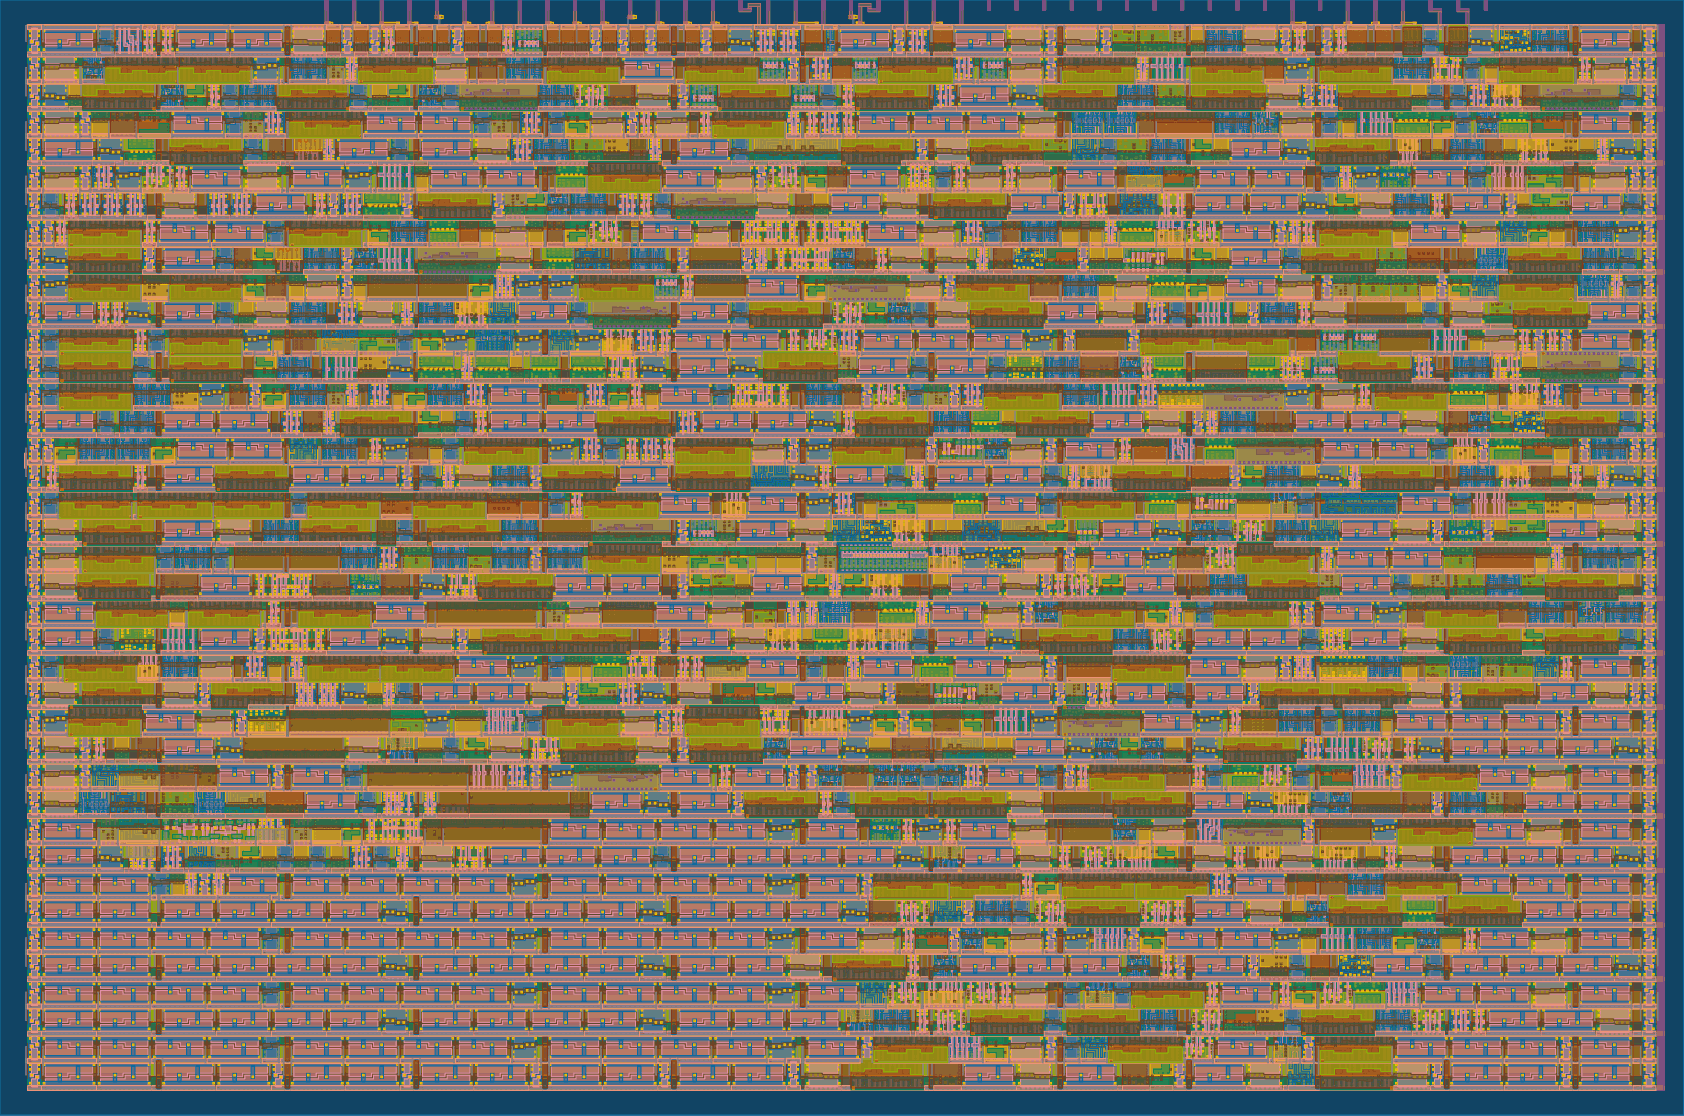
\includegraphics[width=\columnwidth]{./Figs/gh action gds layout.png}
\caption{2D render of a single tile}
\label{fig:render_cells_in_use}
\end{figure}

\begin{figure}[!t]
\centering
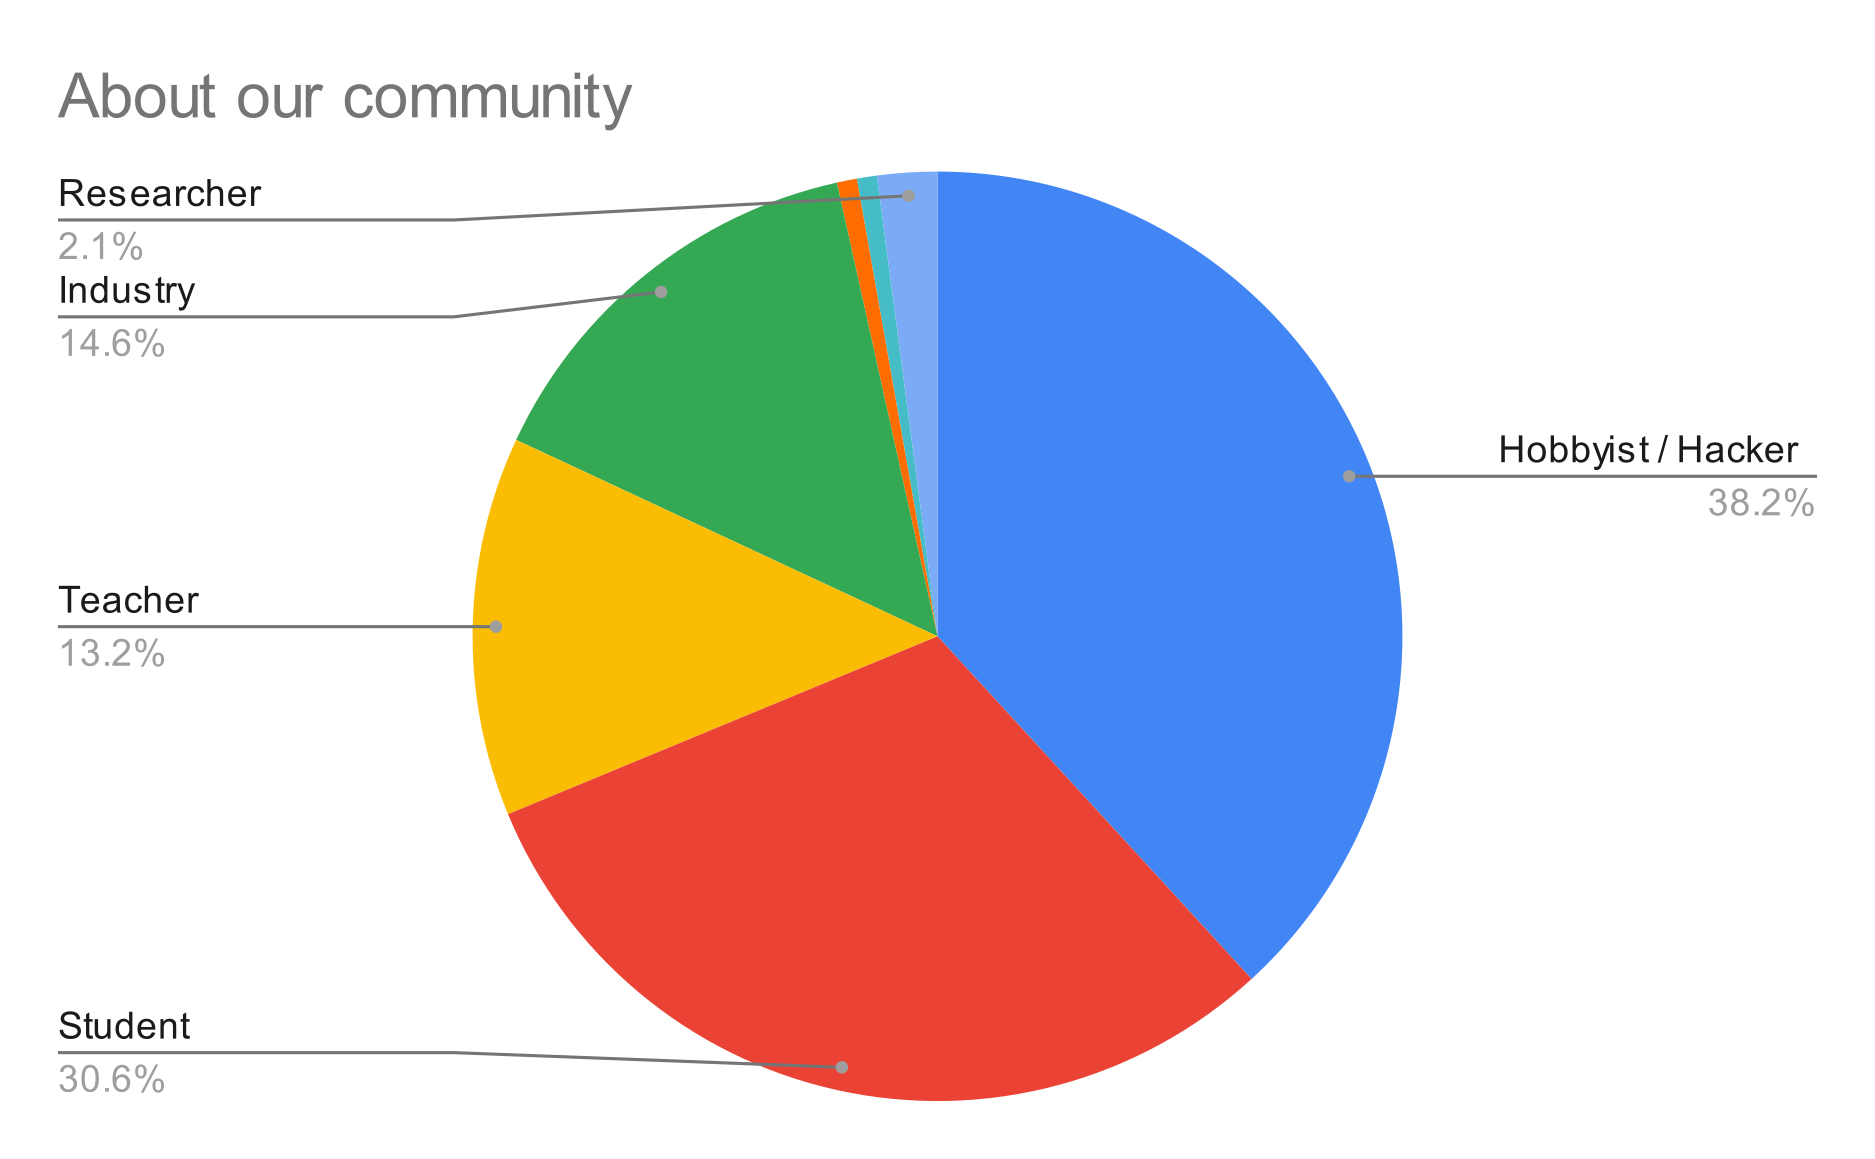
\includegraphics[width=\columnwidth]{./Figs/about our community pie chart.png}
\caption{How TT04 submitters identified themselves.}
\label{fig:TT04_submitters}
\end{figure}

%\section{Design Flow}
\label{sec:design_flow}

Tiny Tapeout designs are primarily developed in the Verilog Hardware Description Language (HDL) or Wokwi~\cite{wokwi}.
Wokwi is a web based visual schematic editor for hardware description, designed as an easier way for individuals with no prior HDL experience to get started.
The Tiny Tapeout website~\cite{tinytapeout} includes a basic Wokwi getting started guide, demonstrating how to use the tool to draw circuits, which is made available in English and Spanish.

The design flow has the participant create a GitHub~\cite{github} source code repository based on provided templates then add their ASIC design. This triggers automated tests and the generation of binary layout files in GDSII~\cite{gds}. If all tests pass and the binary layout files are correctly generated, the design is then submitted to a quarterly shuttle for production in silicon.

The Tiny Tapeout GitHub templates\cite{verilogtemplate} make use of GitHub Actions\cite{githubactions}---an automatic continuous integration system triggered every time the repository is updated. This reduces duplicated effort and makes it possible for Tiny Tapeout to support large numbers of participants without excessive technical overhead.

There are four main jobs in the continuous integration system:

\begin{enumerate}
	\item GDS: installs OpenLane\cite{openlane} and the SkyWater Sky130\cite{skywaterpdk} PDK, builds the binary layout files, and generates a summary of the design (Fig.~\ref{fig:summary_table_GDS_job}). The summary includes utilization, standard cells used, a 2-D render (Fig.~\ref{fig:render_cells_in_use}) and an interactive 3-D viewer (Fig.~\ref{fig:interactive_3D_viewer}).
This job can also optionally run a gate-level verification of the design.
	\item Verification: installs the YosysHQ open source Computer-Aided Design (CAD) suite, which includes many common electronic design automation (EDA) tools; uses iVerilog\cite{iverilog} and cocotb\cite{cocotb} to run included testbenches.
	\item Documentation: generates a preview of the documentation.
	\item Precheck: runs Design Rule Check (DRC) tests to ensure the design can be integrated into the multi project chip.
\end{enumerate}

Successful GDS, Documentation, and Precheck job completion are all required for a design to be submitted to a shuttle for production.
Verification is optional but highly encouraged. Submissions designed in Wokwi are able to make use of its integrated truth table testing system\cite{automatedtesting}.

While the Tiny Tapeout continuous integration system can be run entirely in the user's web browser, it is also possible to install a local copy of the tools\cite{localinstall} on a participant's computer. Locally installed tools can help to reduce the time between design iterations, especially for the test and verification jobs.

\begin{figure}[!t]
\centering
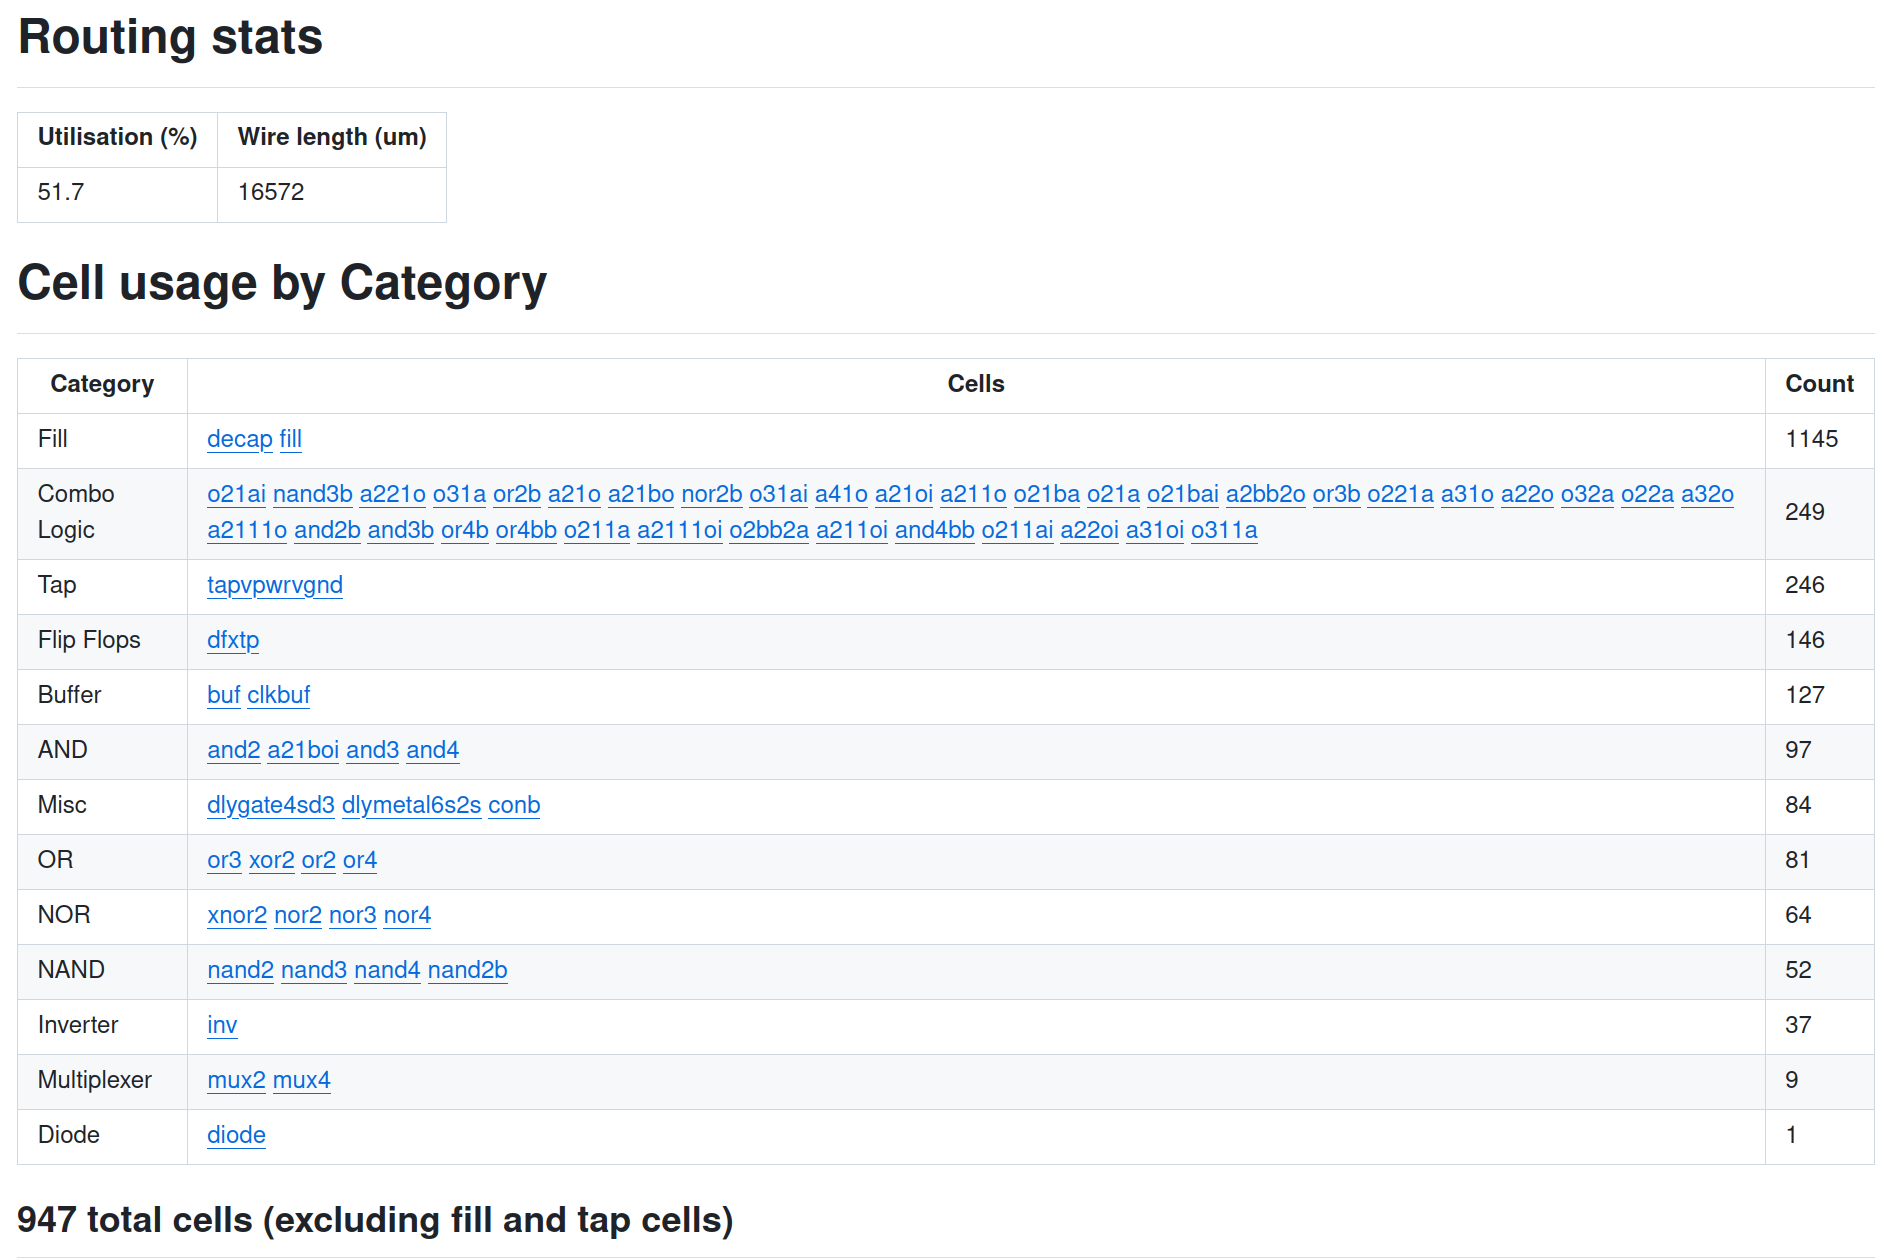
\includegraphics[width=\columnwidth]{./Figs/gh action cell stats.png}
\caption{A summary table from the GDS continuous integration job.}
\label{fig:summary_table_GDS_job}
\end{figure}

\begin{figure}[!t]
\centering
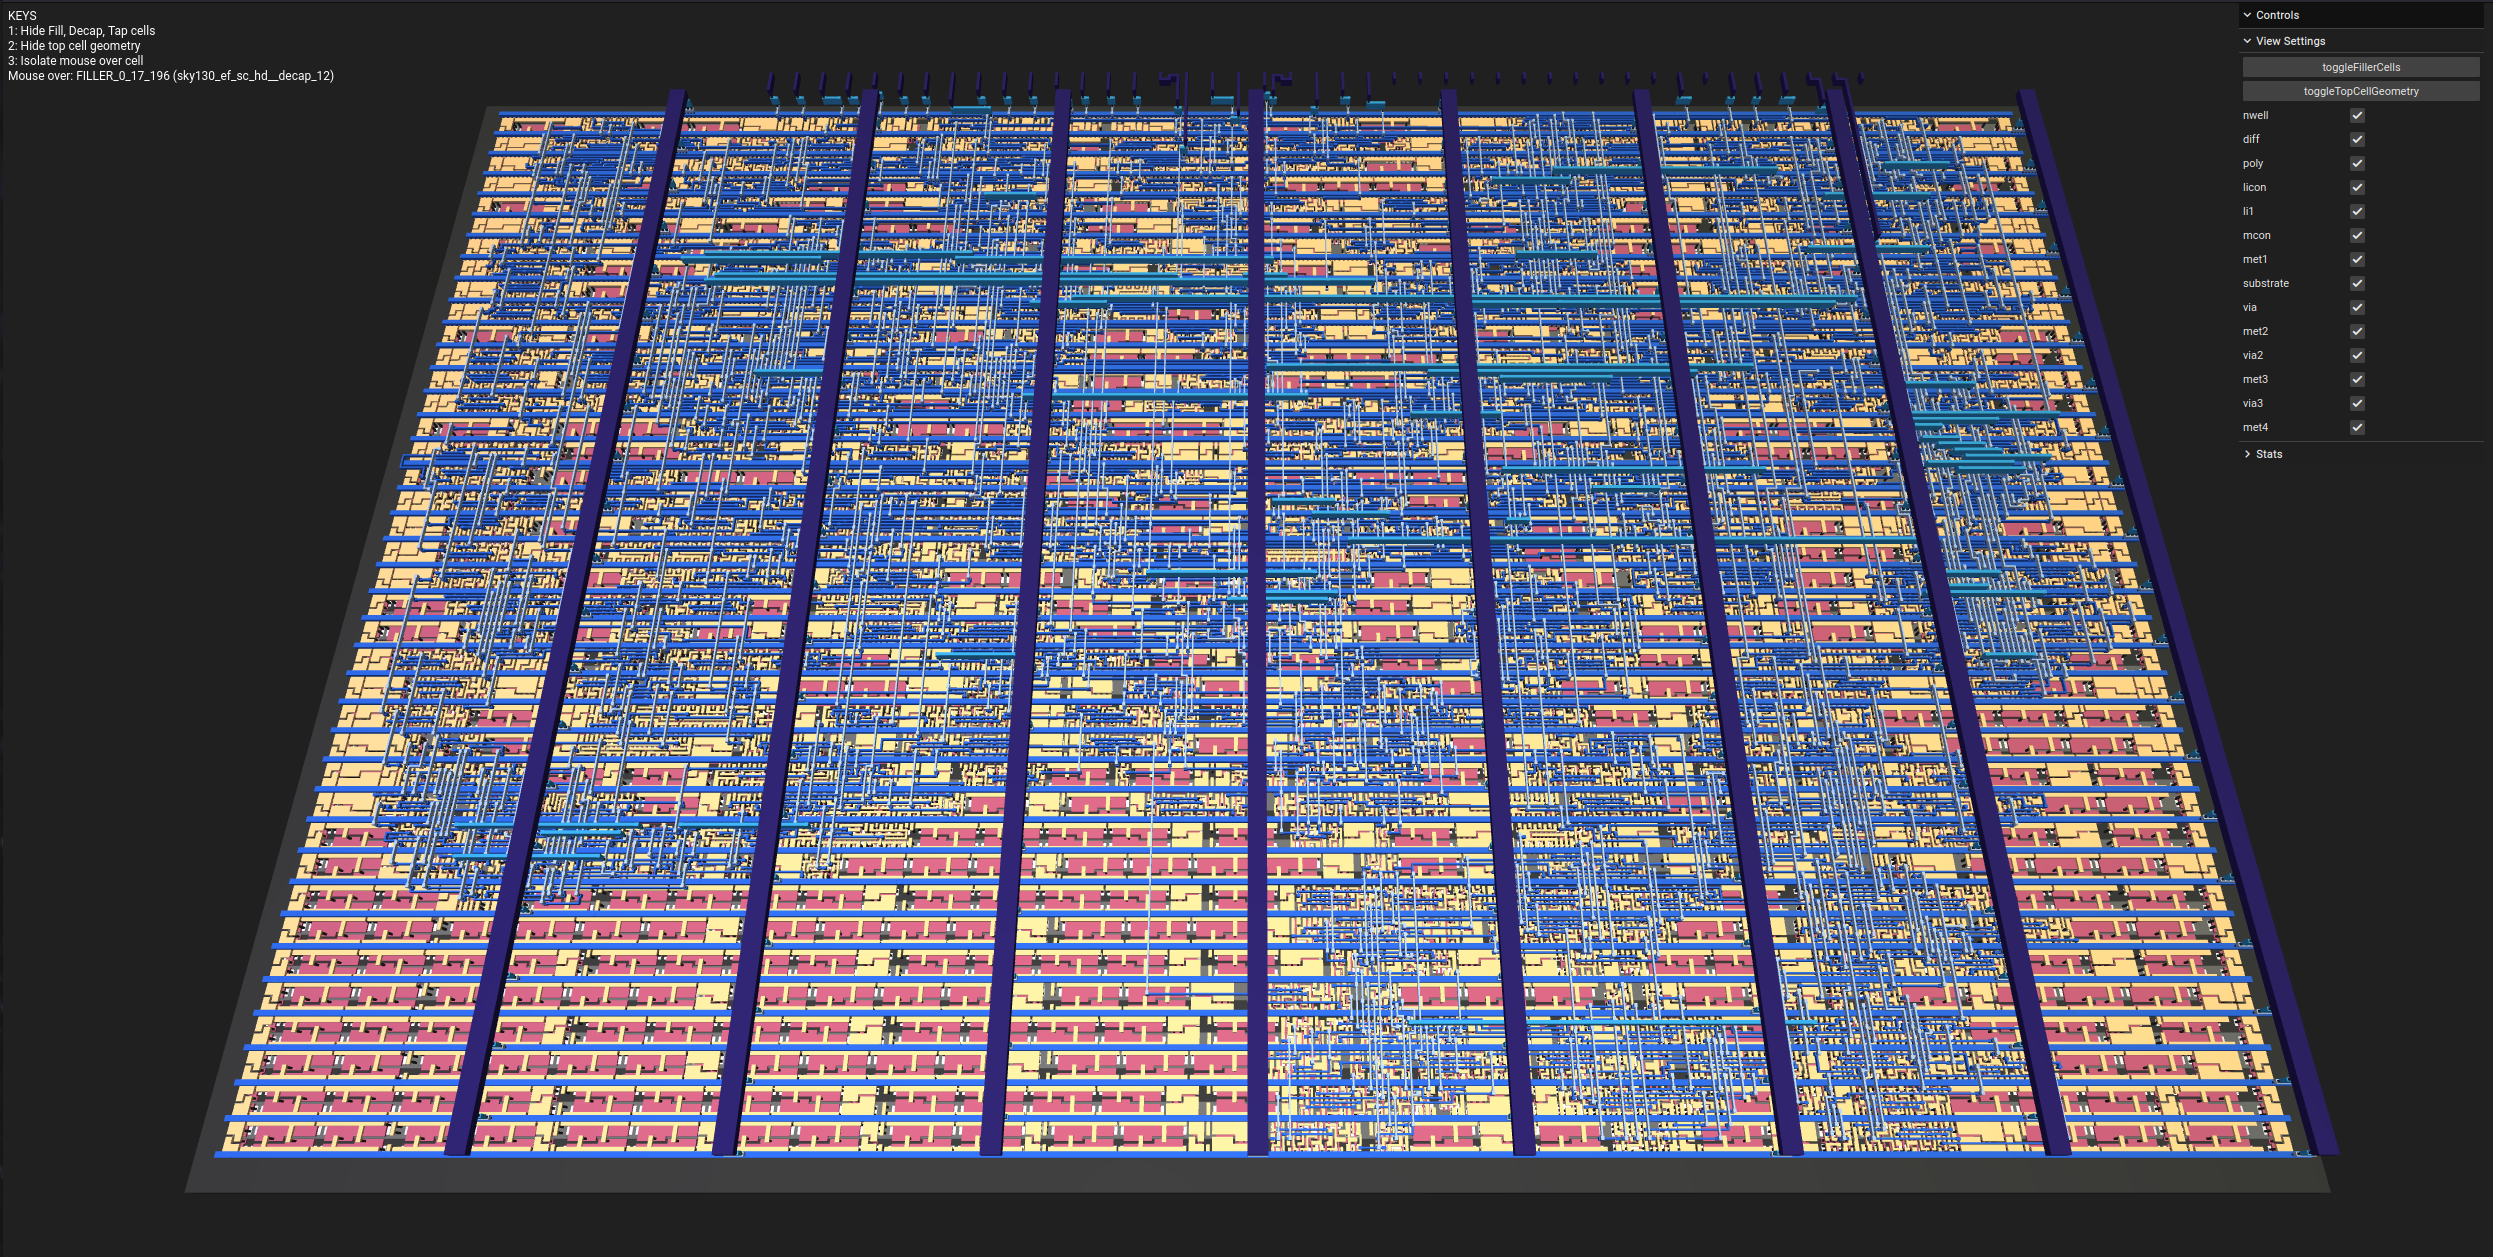
\includegraphics[width=\columnwidth]{./Figs/gh action gds 3d view.png}
\caption{The interactive 3-D viewer.}
\label{fig:interactive_3D_viewer}
\end{figure}

%\section{Scan Chain Architecture}
\label{sec:scanchain_arch}

Tiny Tapeout started as an experiment in fitting as many designs as possible into the \qty{10}{\milli\meter\squared} available on the Google lottery shuttles (Fig.~\ref{fig:500_designs_chain_TT01}).
To rapidly prove the concept, initial designs were based on a scan chain architecture to simplify testing.
Each Tiny Tapeout 01 design has eight inputs and eight outputs.
Clock and reset signals were optional and not treated specially. The chain was formed of scan flops~\cite{skywaterpdk}, a type of flip flop with an multiplexer integrated at its input. An example showing a two design scan chain is shown in Fig.~\ref{fig:simplified_view_2_designs}.

\begin{figure}[!t]
\centering
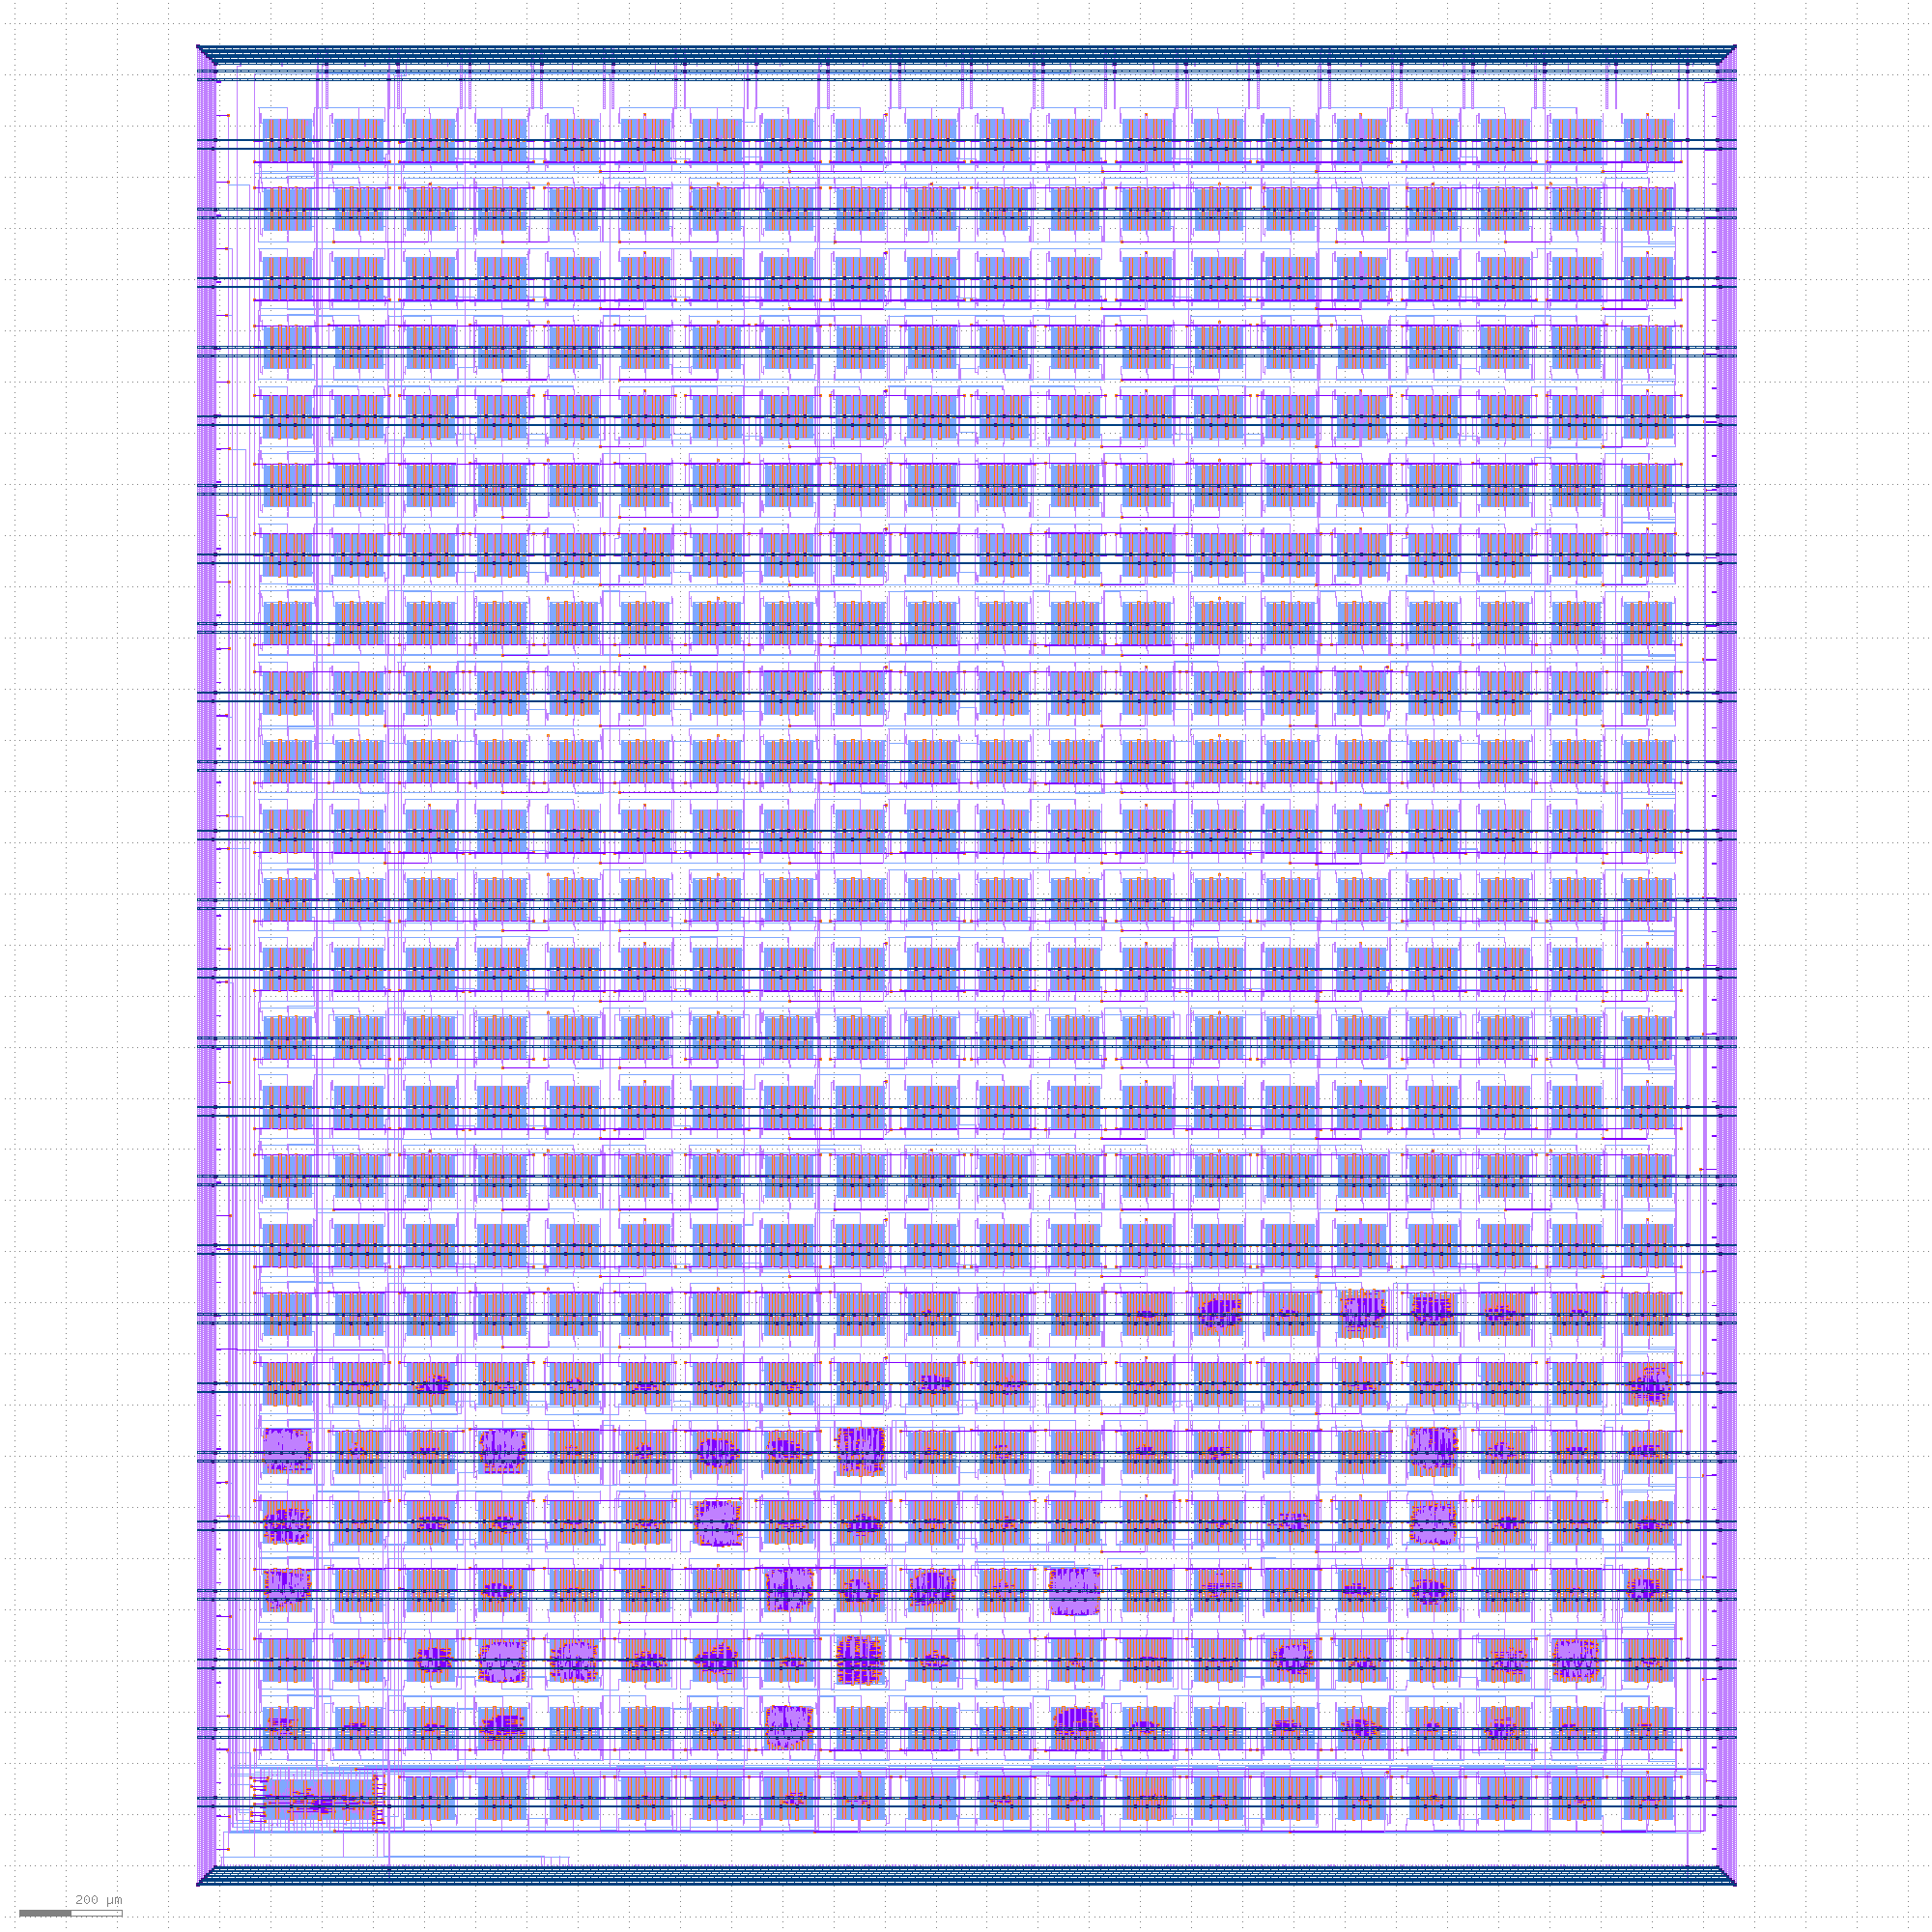
\includegraphics[width=1\columnwidth]{./Figs/tt01_whole_die.png}
\caption{500 designs connected in a chain for Tiny Tapeout 01; the scan chain driver can be seen in the lower left corner.}
\label{fig:500_designs_chain_TT01}
\end{figure}

\begin{figure}[!t]
\centering
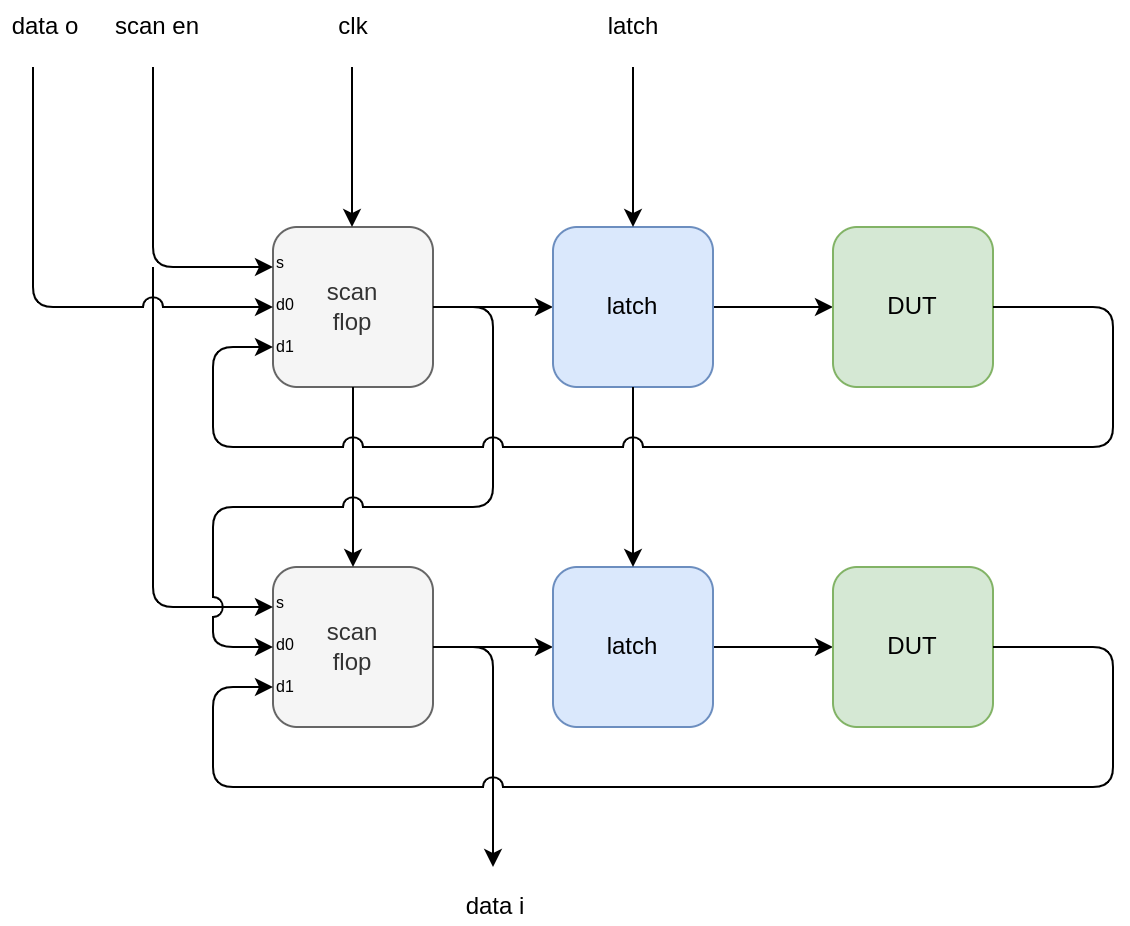
\includegraphics[width=\columnwidth]{./Figs/scanchain_block_diagram.png}
\caption{A simplified view of two Tiny Tapeout 01 designs in the scan chain.}
\label{fig:simplified_view_2_designs}
\end{figure}

Each design sends data into the secondary input of the scan flop and receives its own input from the output of the flop via a latch.
The chain is built~\cite{updateiodesign} by sending data from the output of the previous scan flop into the primary input of the next scan flop.
This arrangement allows the loading of data into any of the designs, followed by the capturing of the output and its clocking through the rest of the chain to the overall chain output.

While relatively easy to implement, a scan chain architecture has a downside: high latency.
As more designs are added to the chain it takes longer to send and receive data through it.
For example: assuming a \qty{50}{\MHz} scan chain clock with 250 designs each having eight inputs and eight outputs, the maximum refresh rate of the resulting chain is $\qty{50}{\MHz} / (8 \times 250) = \qty{25}{\kHz}$.

The Tiny Tapeout 01 scan chain was embedded into each design, meaning a user could unintentionally remove it and break the chain.
This risk was mitigated with a formal~\cite{tinytapeoutscan} equivalence check which proves the chain was present in each submitted design.
For Tiny Tapeout 02 and Tiny Tapeout 03 the scan chain was separated into a discrete macro block which participants cannot modify.

\begin{figure}[!t]
\centering
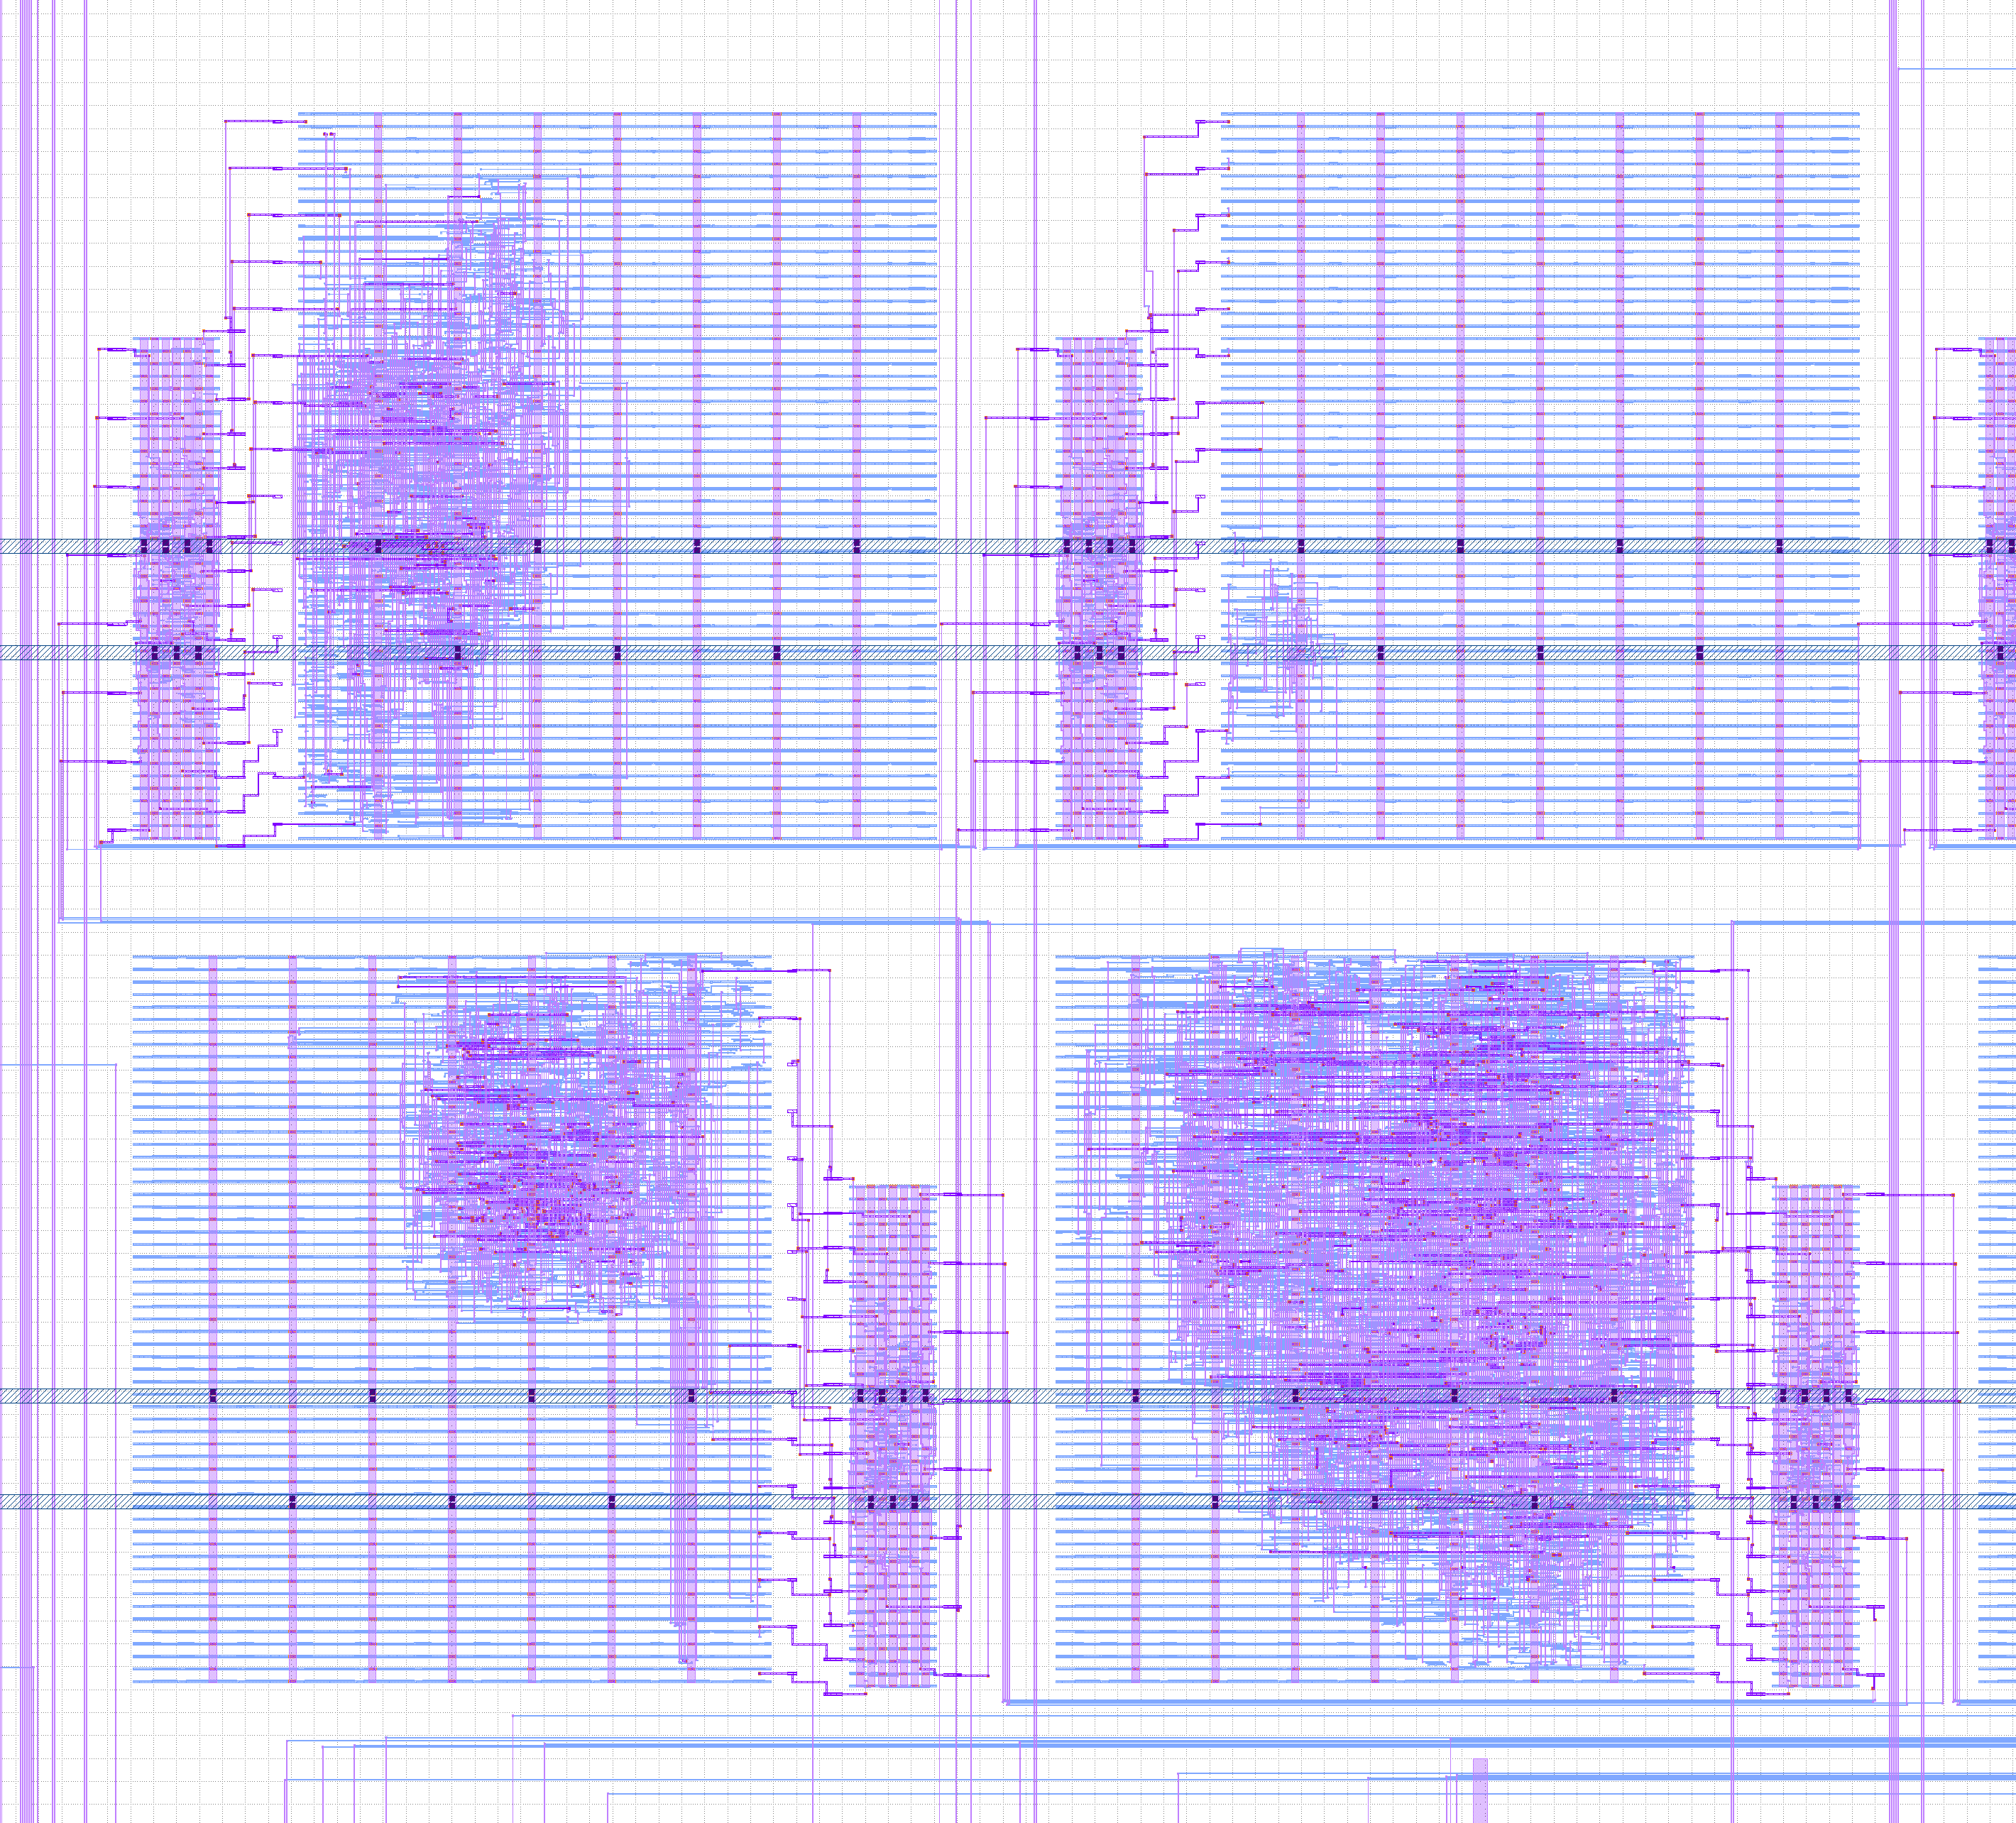
\includegraphics[width=\columnwidth]{./Figs/tt02_gds_zoom.png}
\caption{Tiny Tapeout 02 designs, showing the discrete scan chain blocks.}
\label{fig:TT02_separate_scan_blocks}
\end{figure}

Another concern with the scan chain design was hold violations, due to the large number of serially connected flops and potentially large clock skews over long signal wires. This was mitigated by reclocking the output data with a negative edge (negedge) flop, providing substantially more hold margin.

Following static timing analysis (STA) it was discovered that the clock duty cycle could change substantially due to the \(500\) sequential clock drivers in the chain. Depending on the clock buffers and capacitance between each design the clock duty cycle could either increase or decrease, with this effect accumulated over the chain.

For Tiny Tapeout 01 and Tiny Tapeout 02 each design used two clock buffers, with the internal flops driven after the first buffer.
Tiny Tapeout 03 used inverting clock buffers, with only one between the clock input and output. Fig. ~\ref{fig:TT02_vs_TT03} shows a comparison between the TT02 and TT03 clock buffer designs. By inverting the clock between each design any asymmetry in the clock pulse is evenly spread across the negative and positive cycles.

\begin{figure}[!t]
\centering
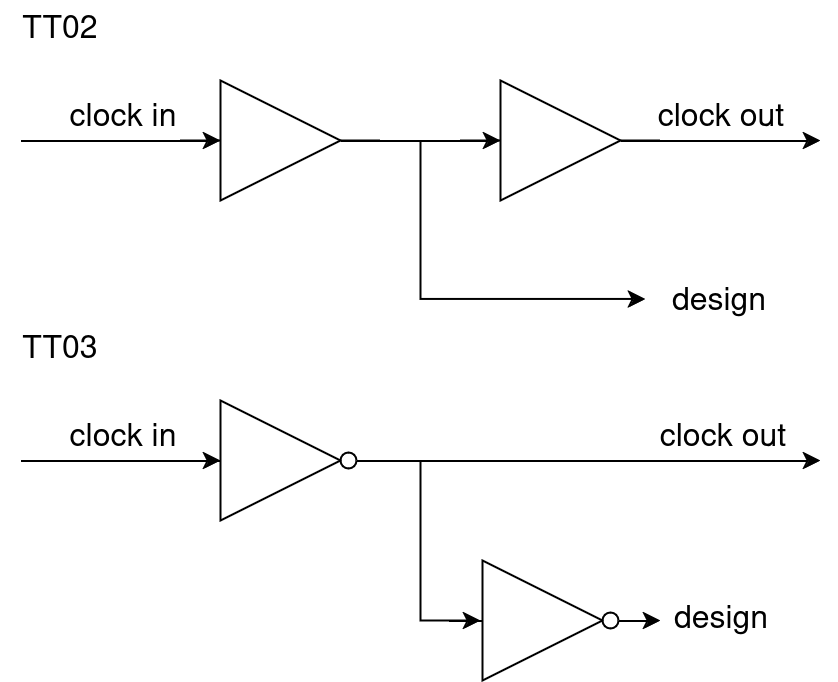
\includegraphics[width=\columnwidth]{./Figs/tt02 vs tt03 scanchain clock.png}
\caption{The Tiny Tapeout 03 architecture buffers the output from the clock network into each design. Clock polarity is alternated between designs to minimize asymmetry between positive and negative cycles.}
\label{fig:TT02_vs_TT03}
\end{figure}

The verification effort~\cite{verificationmd} for the scan chain was broad and included a community review, register transfer level (RTL) and gate level (GL) simulation, formal verification\cite{sby}, STA, layout vs. schematic (LVS), DRC, and device level static verification~\cite{cvc}.

%\section{Circuit Boards}
\label{sec:circuit_board}
After manufacture, the chips are mounted onto small carrier boards with 0.1~inch headers. This allows people with limited surface mount technology (SMT) assembly experience to build their own demonstration boards.

The carrier fits onto the demonstration board shown in Fig.~\ref{fig:demonstration_board}. The demonstration boards are designed primarily for ease of use by beginners, with enough flexibility for power users. As all signals are below \qty{50}{\MHz}, no special layout was needed.

The demonstration board provides:
\begin{itemize}
\item USB-C for power connection,
\item \qty{1.8}{\V} and \qty{3.3}{\V} power supplies for core and IO,
\item \qty{20}{\MHz} oscillator,
\item Buttons for reset and single-step clock,
\item An 8-way DIP switch for inputs,
\item A 9-way DIP switch for design selection,
\item A 7-segment LED display for the outputs,
\item Headers for all IO, including 2 standard Digilent ports (PMOD),
\item A header to select the internal clock or provide one externally,
\item A header to select internal or external scan chain driver,
\item A header to engage an automatic clock divider in input pin 0.
\end{itemize}

\begin{figure}[!t]
\centering
\includegraphics[width=0.5\textwidth]{./Figs/tt02 pcb assembled.JPG}
\caption{The demonstration board. Certified Open Source Hardware ES000040~\cite{oshwacertification}.}
\label{fig:demonstration_board}
\end{figure}

%\section{Scan Chain Silicon Results}
\label{sec:scan_chain_res}

Tiny Tapeout 02 chips were received in October 2023, 11 months after the chips were submitted for manufacture on the Efabless chipIgnite 2211Q shuttle.
The chips were tested for the first time on a public livestream~\cite{siliconalive}.
During this testing the chain was validated and a small number of the designs were demonstrated to be working.
In further testing following the livestream another 30 designs were and shown to be working.

\begin{figure}[!t]
\centering
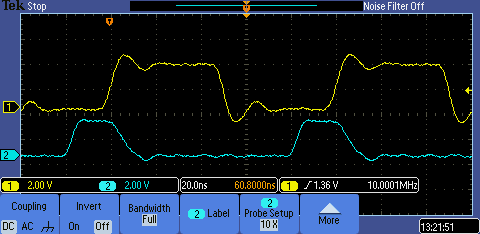
\includegraphics[width=\columnwidth]{./Figs/tt02_clock_out.png}
\caption{Measurement from Tiny Tapeout 02 silicon, with input clock in yellow and the distorted output clock in blue.}
\label{fig:TT02_clock_out}
\end{figure}

After measuring the clock asymmetry (Fig.~\ref{fig:TT02_clock_out}) and maximum frequency it was decided to run the production boards with a \qty{20}{\MHz} oscillator, resulting in a \qty{10}{\MHz} scan chain clock and a \qty{5}{\kHz} IO update rate in order to maximize stability.

Some Tiny Tapeout 02 designs did not function as expected; in most cases this was determineted to be due to faults in the submitted design.

Of the designs submitted 82 used the Verilog HDL, 64 were created using the Wokwi graphical editor, and six used alternative HDLs including VHDL, Amaranth~\cite{amaranth}, and Chisel~\cite{chisel}.

Some of the designs created using Wokwi using combinational logic in clock paths (Fig.~\ref{fig:failed_design_comb_logic}) worked in simulation but failed in hardware.
This was determinted to be due to the lack of timing data in the simulation, and wasn not detected by STA because the clock paths were not known. A detailed analysis on these failures has yet to be carried out.

\begin{figure}[!t]
\centering
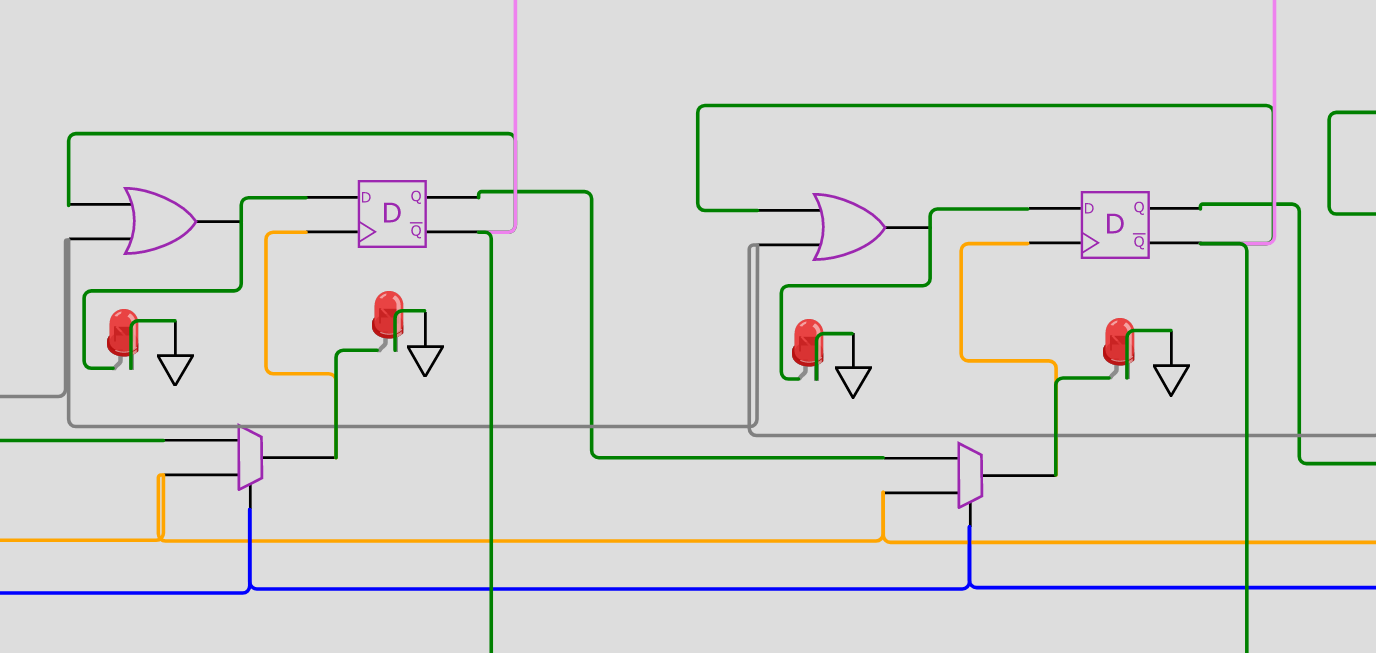
\includegraphics[width=\columnwidth]{./Figs/wokwi mux clock logic.png}
\caption{Combinational logic in the clock path of one of the failed designs.}
\label{fig:failed_design_comb_logic}
\end{figure}

At the time of writing, PCBs are in production and are expected to ship to customers by the end of January 2024.

Silicon from Tiny Tapeout 3 production was received in January 2024. The updated scan chain design shows a more symmetric output clock at the end of the chain (Fig.~\ref{fig:TT03_silicon_measurement}). The improved clock symmetry will allow for the use of a faster scan chain clock, resulting in a faster update frequency.

\begin{figure}[!t]
\centering
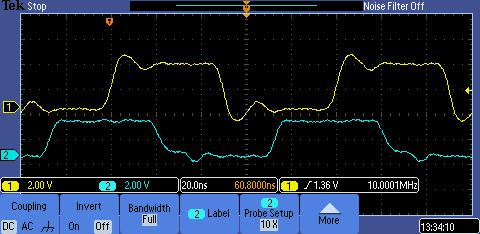
\includegraphics[width=\columnwidth]{./Figs/tt03_clock_out.png}
\caption{Measurement from Tiny Tapeout 03 silicon.}
\label{fig:TT03_silicon_measurement}
\end{figure}

%\section{Beyond the Scan Chain}
\label{sec:beyond_scanchain}
The biggest limitation of the scan chain based architecture was the IO bandwidth and latency.
For TinyTapeout 4 a new architecture was needed, and a series of proposals was gathered from the community.
An online video call was held and the 10 proposals discussed.
The winning design was a fairly straightforward multiplexer design shown in Fig.~\ref{fig:multiplexer_design}.

\begin{figure}[!t]
\centering
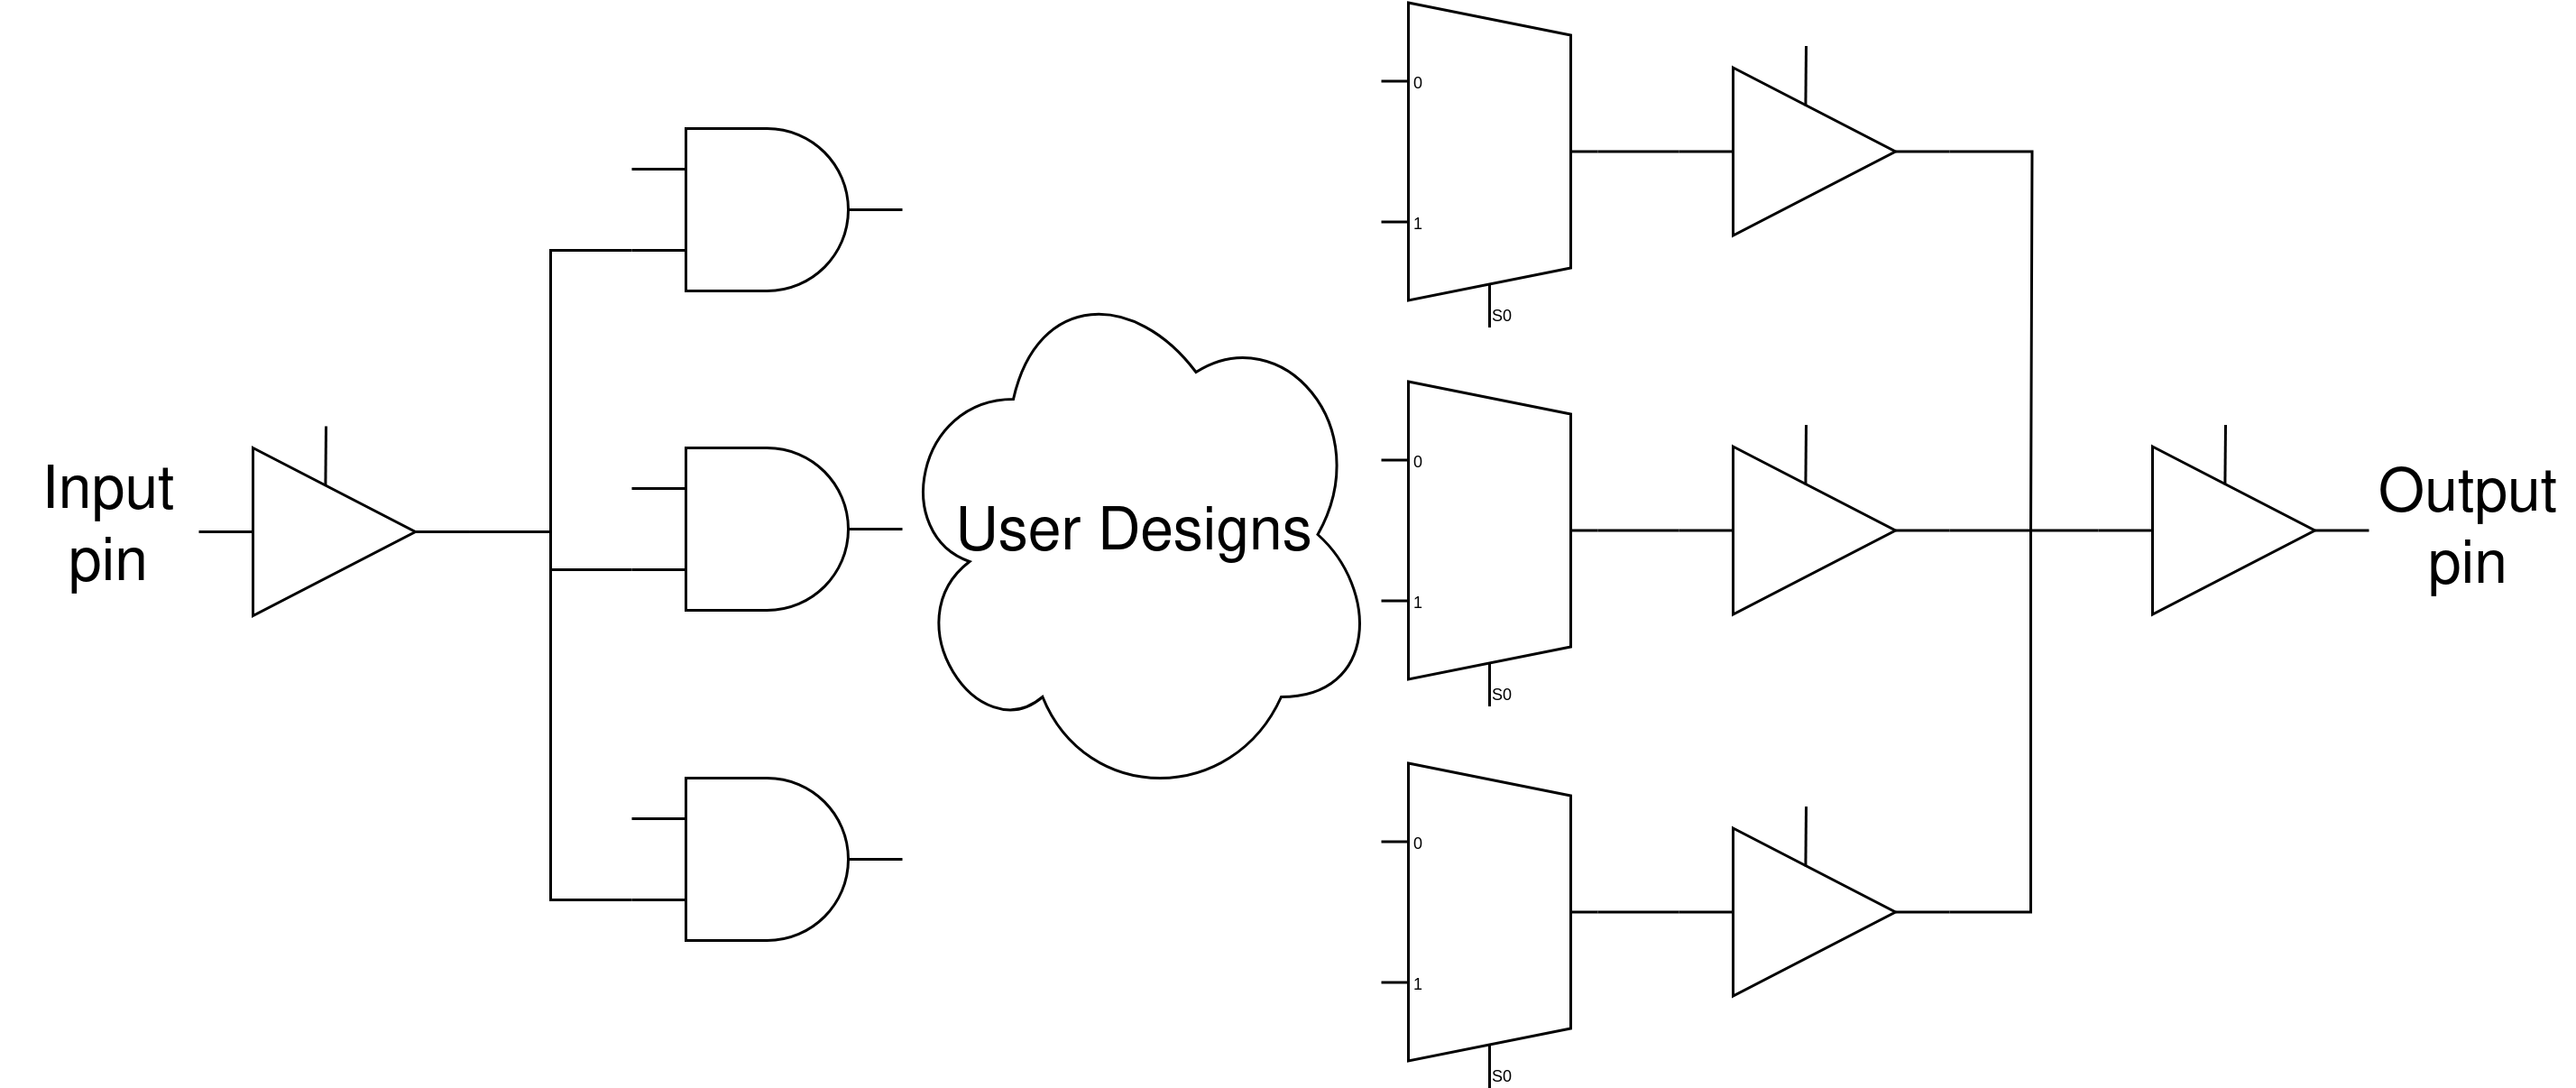
\includegraphics[width=\columnwidth]{./Figs/mux architecture.png}
\caption{Simplified diagram of the multiplexer architecture.}
\label{fig:multiplexer_design}
\end{figure}

The physical layout (shown in Fig.~\ref{fig:TT03_5_test_design}) consists of a central controller connected up and down to two vertical spines.
Twenty-four horizontal muxes connect to the spine with each supporting 16 designs.
This allows up to 384 separate single tile designs.
Multiple tile designs were also enabled, allowing a maximum project size of $8 \times 2$ tiles or $1359 \times \qty{225}{\um\squared}$---around \num{20000} logic cells. Table~\ref{tab:comparison_TT03_TT04} shows the key differences between TT03 and TT04.

\begin{figure}[!t]
\centering
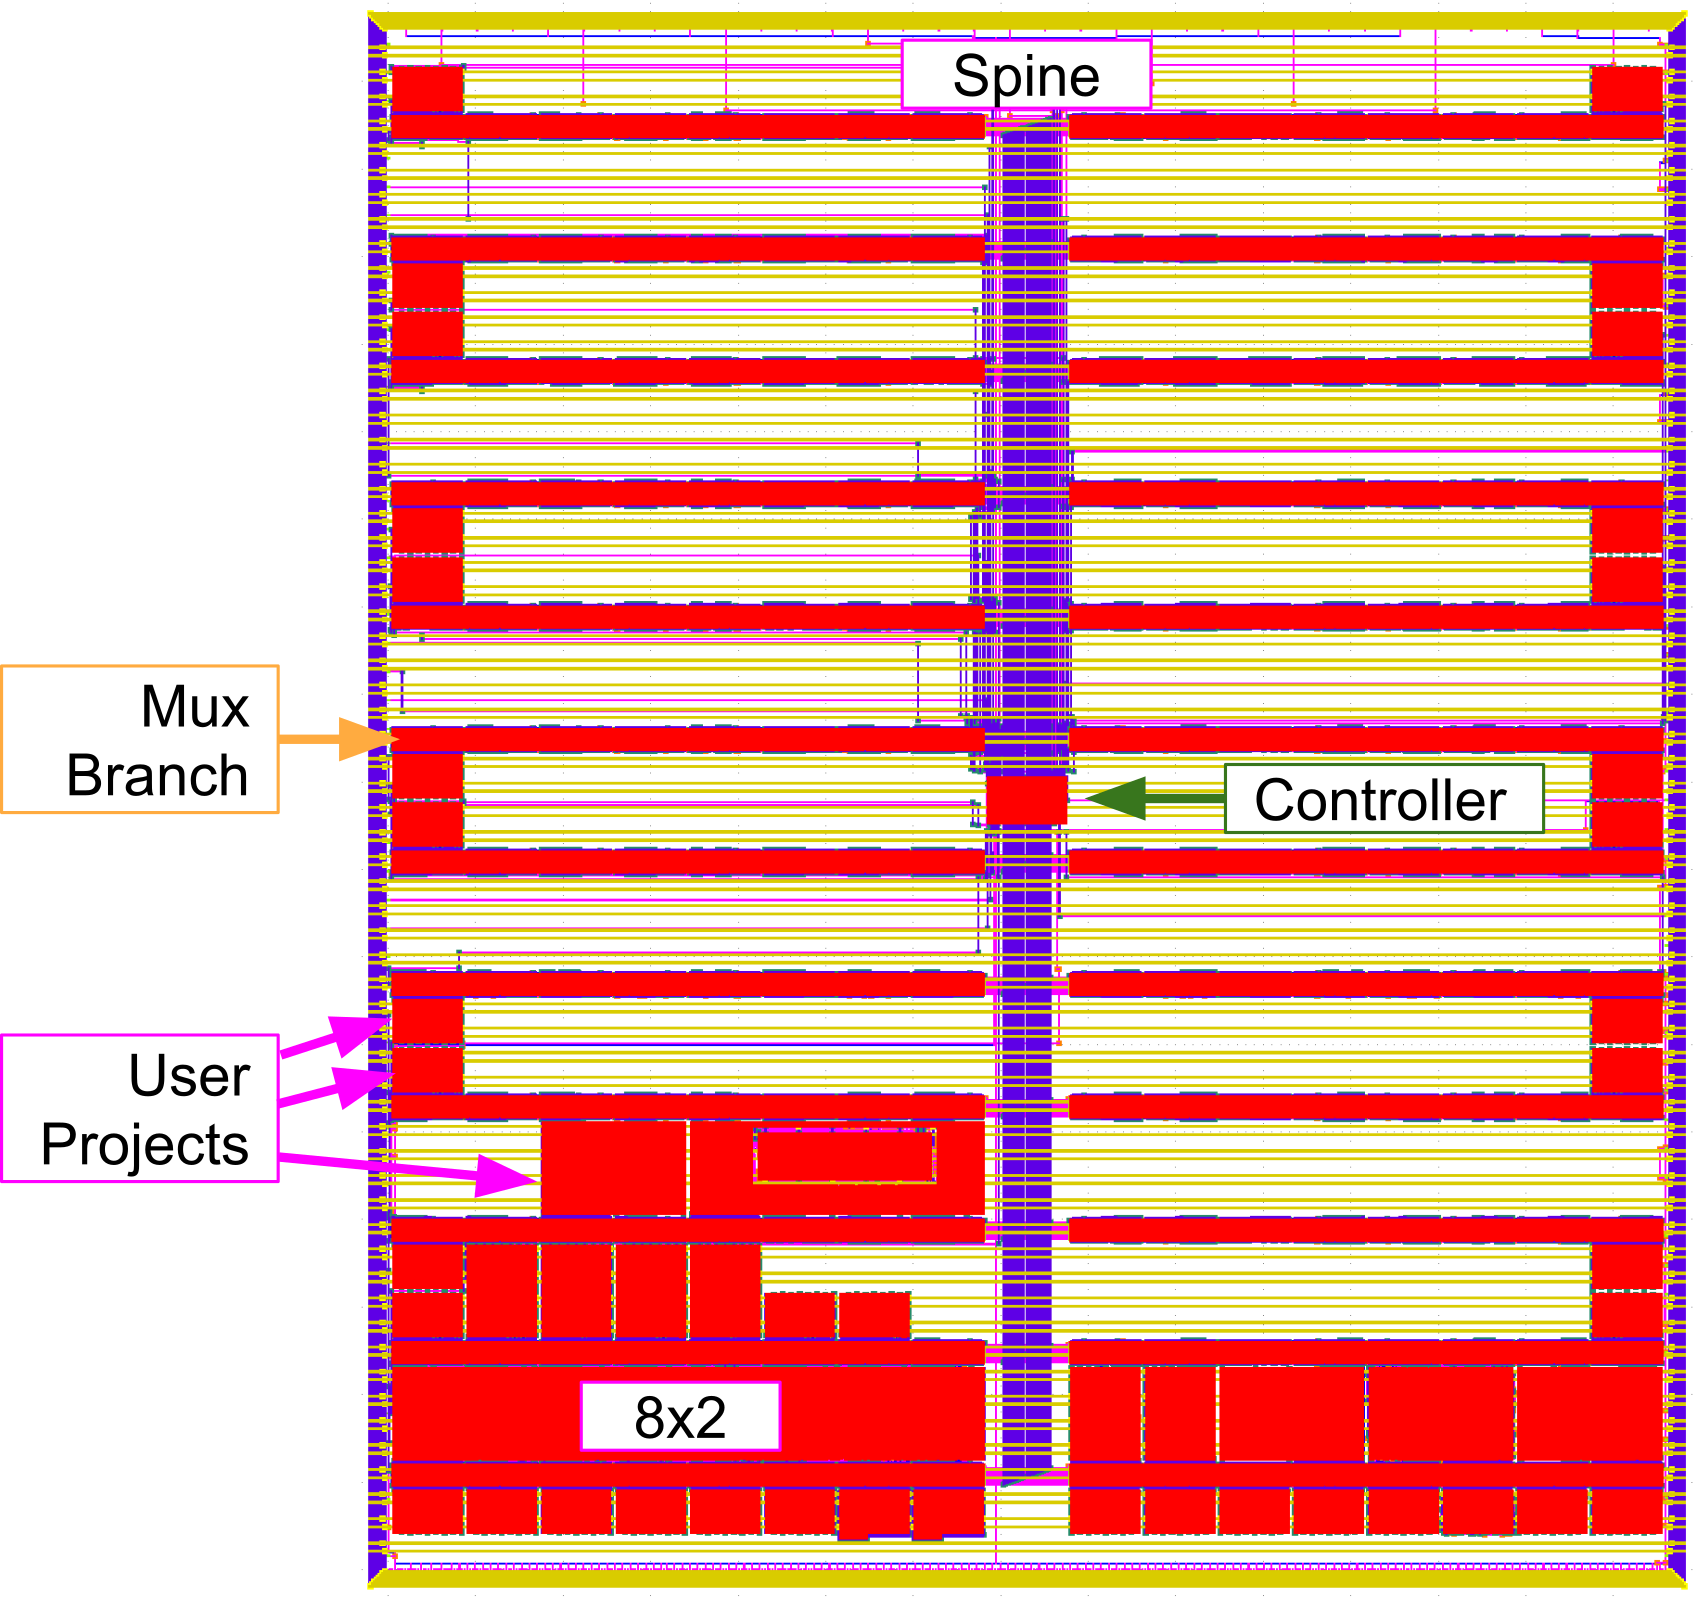
\includegraphics[width=\columnwidth]{./Figs/tt3p5 layout.png}
\caption{The TT03.5 test design.}
\label{fig:TT03_5_test_design}
\end{figure}

Another major limitation of TT01 to TT03 was the small number of IO.
The scan controller used 9 GPIOs to select the currently active design, which, while simplifying the demo board, wasted valuable pins.
With TT04, the parallel design selection was dropped in favor of a serial protocol.
The extra pins were then used as bidirectional pins, giving each design clock, reset, and 24 IO.

\begin{table}[!t]
\centering
\caption{Comparison between TT03 and TT04}
\label{tab:comparison_TT03_TT04}
\begin{tabular}{@{}lcc@{}}
\toprule
Parameters & TT03 & TT04 \\
\midrule
Max clock speed & \qty{12.5}{\kHz} & \qty{50}{\MHz} \\
Max design size & $150 \times \qty{170}{\um\squared}$ & $1359 \times \qty{225}{\um\squared}$ \\
Input pins & 8 & 10 \\
Output pins & 8 & 8 \\
Bidirectional I/O pins & None & 8 \\
Custom GDS file & \xmark & \checkmark \\
\bottomrule
\end{tabular}
\end{table}

An invite-only experimental shuttle~\cite{tinytapeout03p5} was submitted with 32 designs to Efabless chipIgnite 2306C.
Two of the designs included a power gate as a stepping stone to supporting analog and mixed-signal designs.

%\section{Multiplexer Silicon Results}
\label{sec:multiplexer_silicon_res}
After silicon was received, the worst round trip latency was measured to be \(20 ns\).

\begin{figure}[htp]
\centering
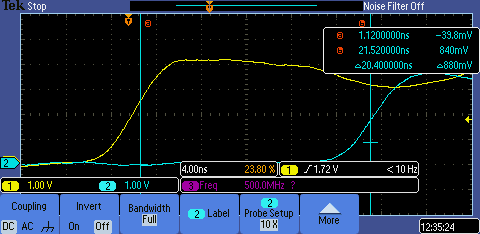
\includegraphics[width=\columnwidth]{./Figs/tt3p5 rising latency.PNG}
\caption{Round trip latency on a rising edge of about \(20 ns\).}
\label{fig:round_trip_latency_rising_edge}
\end{figure}

\begin{figure}[htp]
\centering
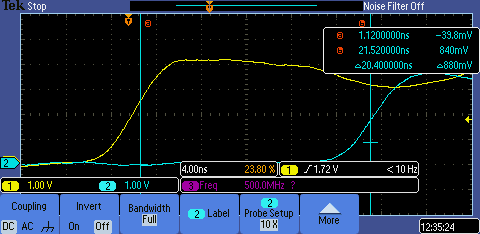
\includegraphics[width=\columnwidth]{./Figs/tt3p5 rising latency.PNG}
\caption{Round trip latency on a falling edge of about \(16 ns\).}
\label{fig:round_trip_latency_falling_edge}
\end{figure}

The new chip pinout and serial design selection required a new demo board that included an easy way to select the design.
The RP2040 microcontroller was chosen as a co-processor as it allows:
\begin{itemize}
\item Drag and drop firmware updates on any OS,
\item Runs MicroPython\cite{micropython}, ideal for beginners to test their designs,
\item External memory emulation via PIO and DMA.
\end{itemize}

\begin{figure}[htp]
\centering
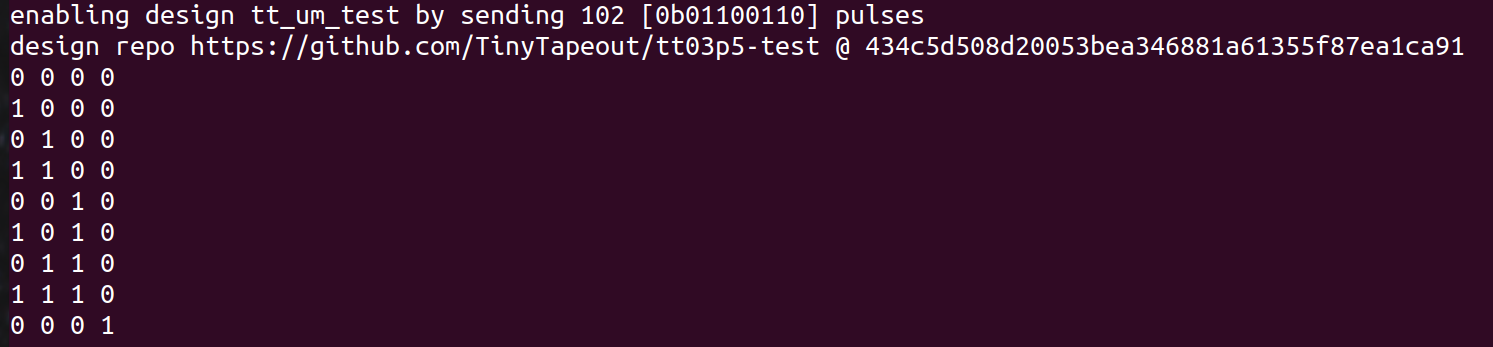
\includegraphics[width=\columnwidth]{./Figs/tt3p5 enable design.png}
\caption{A MicroPython program enabling a design, clocking it, and printing the results.}
\label{fig:micropython_program}
\end{figure}

\begin{figure}[htp]
\centering
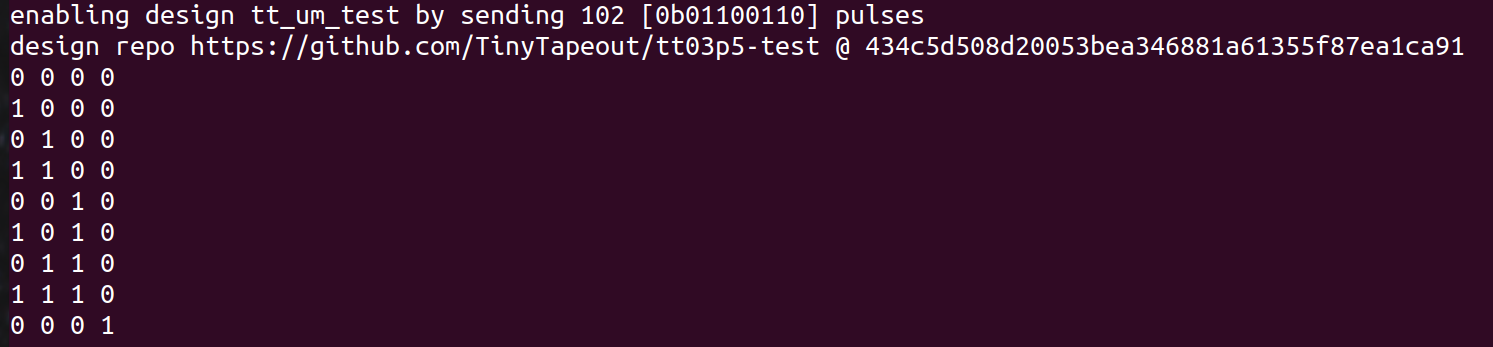
\includegraphics[width=\columnwidth]{./Figs/tt3p5 enable design.png}
\caption{The TT04+ demo board.}
\label{fig:TT04plus_demo_board}
\end{figure}

An additional PMOD expansion port was added for the bidirectional pins, and the community has started to standardize on pinouts~\cite{pinouts} making it easier to test each other's designs.
A new repository was created to house user-contributed PMODs~\cite{awesomepmods}.

\begin{figure}[htp]
\centering
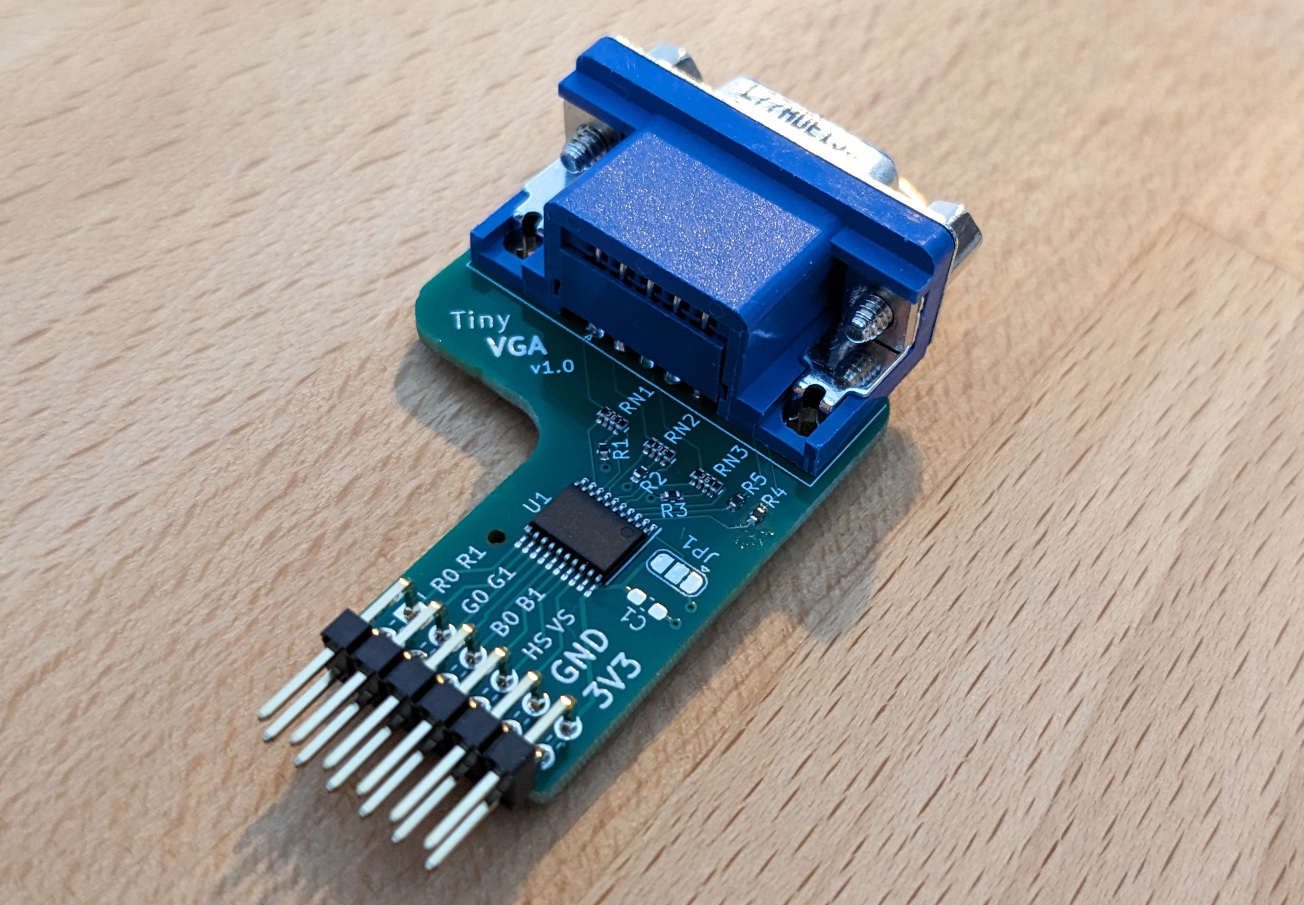
\includegraphics[width=\columnwidth]{./Figs/tiny_vga_pmod.jpg}
\caption{A user-contributed VGA output PMOD.}
\label{fig:user_contributed_VGA_PMOD}
\end{figure}

\begin{figure}[htp]
\centering
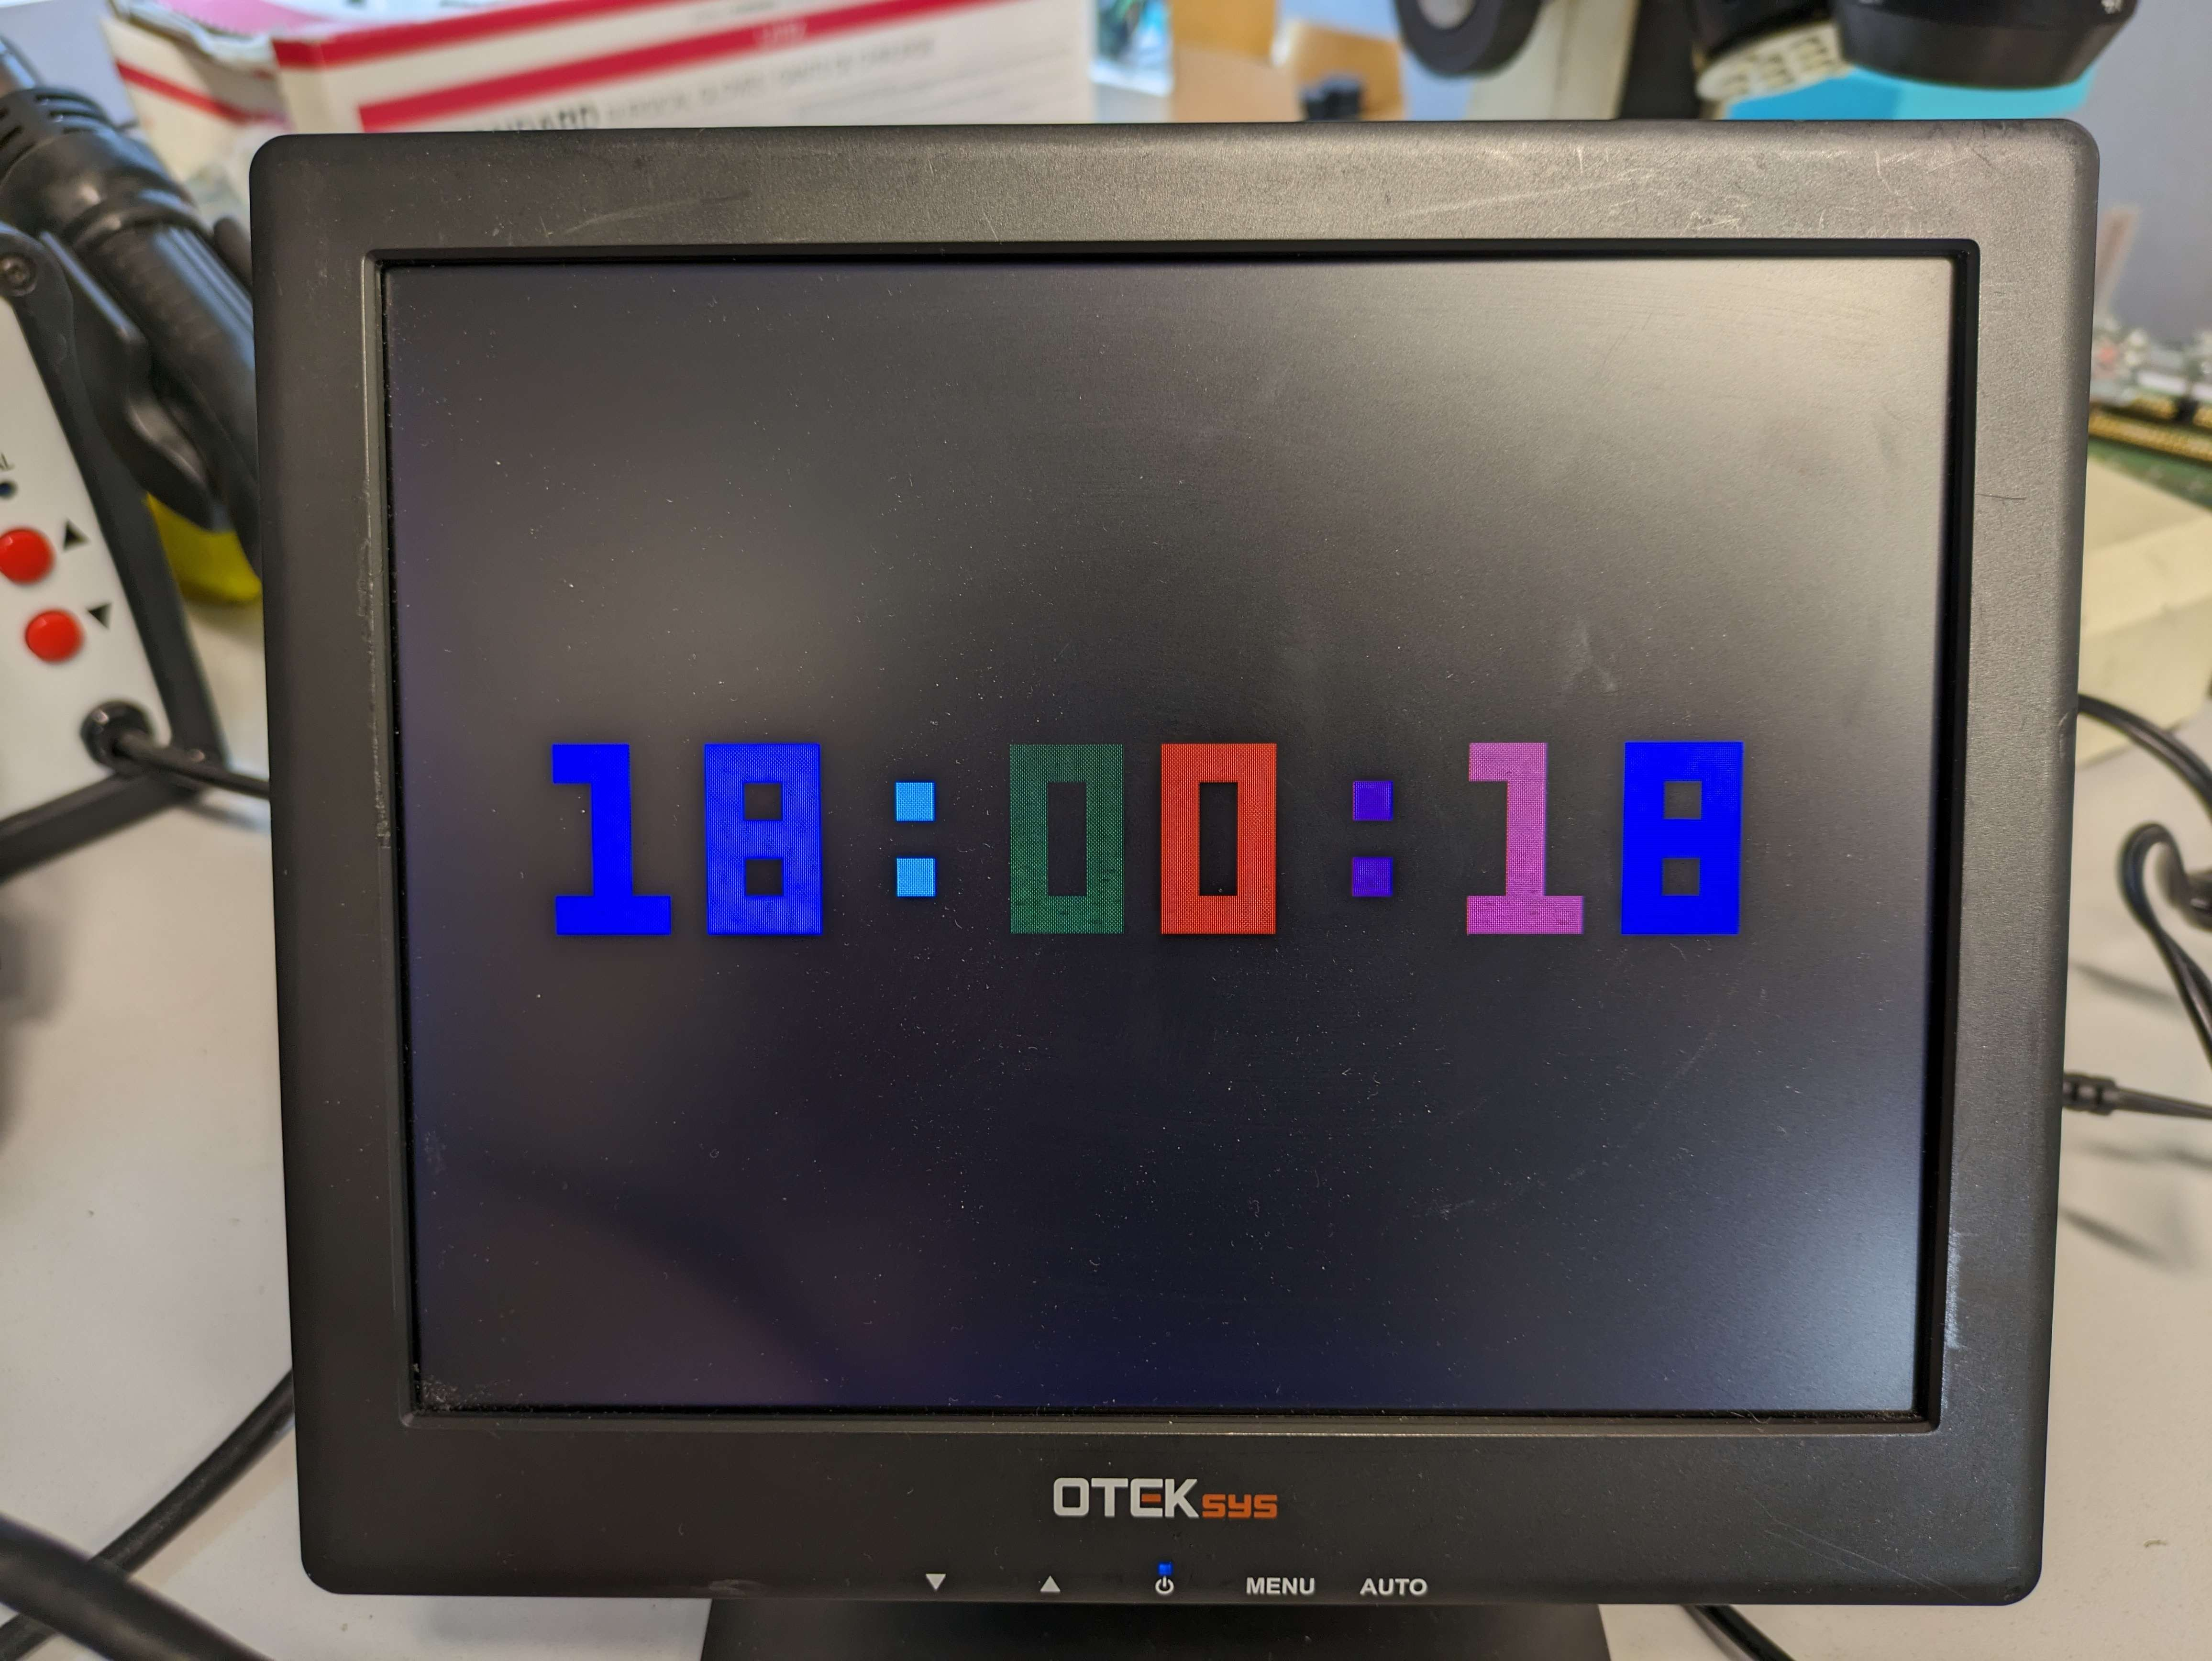
\includegraphics[width=\columnwidth]{./Figs/tt3p5 vga clock.jpg}
\caption{VGA clock design running on TT03.5 silicon.}
\label{fig:VGA_clock_design_TT03_5_silicon}
\end{figure}


%\section{Improving the Multiplexer and Mixed Signal Support}
\label{sec:improving}

Tiny Tapeout 05 split the multiplexer into two parts in order to improve performance. As a result of the split the controller was also updated to multiplex between the two halves.
Some other small changes to the multiplexer include the tweaking, addition, or removal of buffers to improve the STA results.

As each spine segment in Tiny Tapeout 05 is now half as long as in Tiny Tapeout 04, it will exhibit half the capacitance. As a result, we expect to see the round trip latency reduced to around \qty{10}{\ns}.

For Tiny Tapeout 06 the Caravel harness will be replaced by OpenFrame~\cite{openframe}, an alternative harness provided by Efabless that uses the same padring but removes the RISC-V coprocessor.
This results in an additional \qty{5}{\mm\squared} of space for user designs, and 12 more IO pins which will be used for analog signals.

For increased safety, all designs will be power-gated. This allows designers to take more risks in their submissions, or to use custom flows not previously used in Tiny Tapeout.

Analog and mixed signal designs will be enabled by adding an analog multiplexer based on transmission gates~\cite{transmissiongates}. 
This allows up to 192 designs to share the analog pins between them.
These transmission gates were tested as part of an experimental analog submission to Tiny Tapeout 05, shown in Fig.~\ref{fig:transmission_gate_TT05}.

Noise coupling between analog and digital power domains is a known concern. However, due to other limitations of our current setup including its limited number of low bandwidth analog interfaces, we target educational low to medium performance analog and mixed signal designs where noise coupling is a lesser concern.

\begin{figure}[!t]
\centering
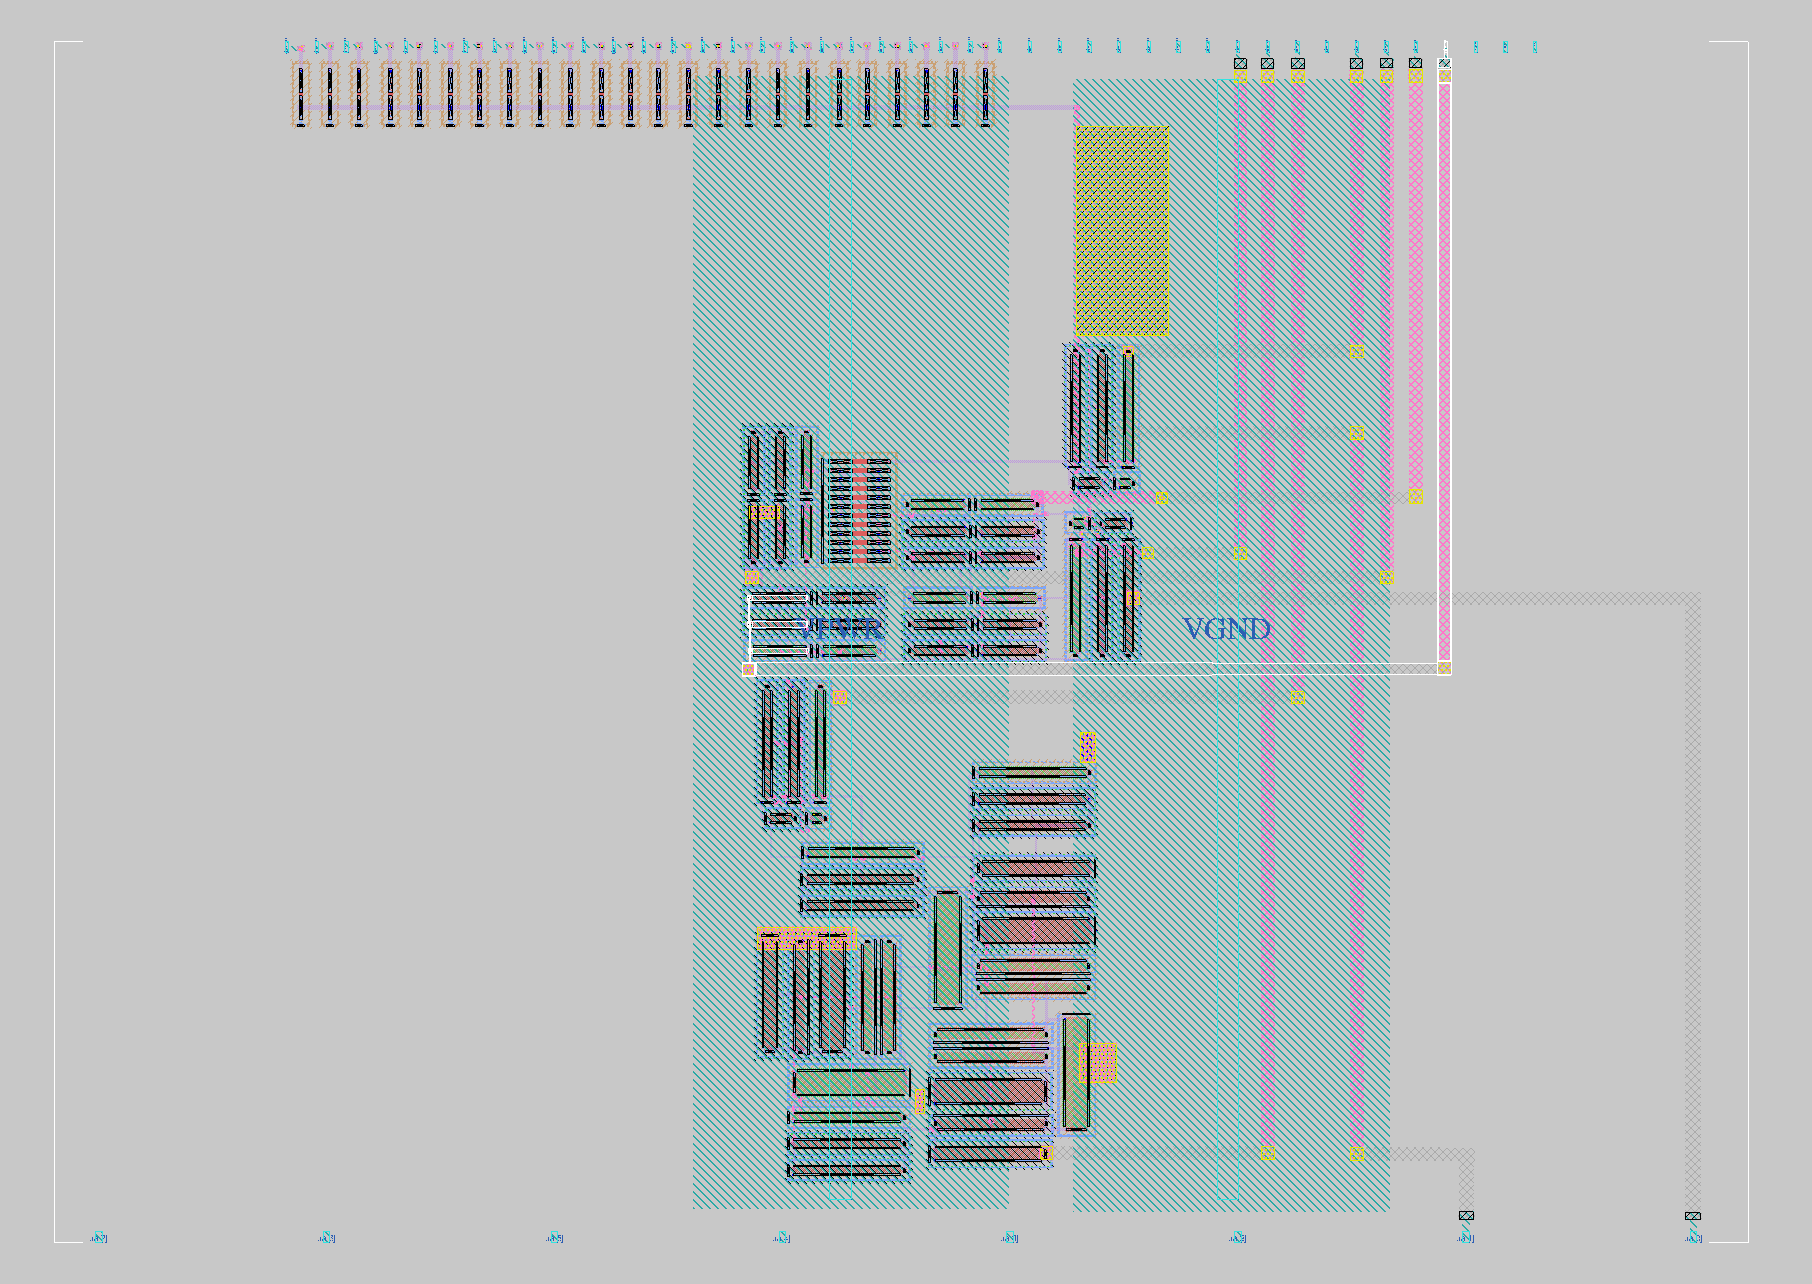
\includegraphics[width=\columnwidth]{./Figs/tt05_transmission_gate.png}
\caption{A ring oscillator and digital to analog converter (DAC) design submitted to Tiny Tapeout 05, with a transmission gate highlighted. This design was automatically placed and routed using an experimental analog place and route (P\&R) tool).}
\label{fig:transmission_gate_TT05}
\end{figure}

Tiny Tapeout 06 is planned to open for submission of digital designs at the end of January 2024, for analog designs at the end of February 2024, and to close for submissions on 19 April 2024.

%\section{Silicon Showcase}
\label{sec:silicon_showcase}

A curated list showcasing the types of designs possible through Tiny Tapeout is provided below:

\begin{itemize}
    \item Serial FPGA~\cite{showcaseserialfpga}, a one fracturable 5-LUT that receives FPGA LUT configuration frames, serially evaluates LUT inputs and LUT outputs.
    \item Synthesizable digital temperature sensor~\cite{showcasetempsense}. By creatively twisting the use of a tristate-inverter (EINVP) a voltage DAC is built. This voltage-mode DAC is used to bias an NMOS into subthreshold operation to discharge the input capacitor of an inverter. Since the subthreshold current of a MOSFET is a strong function of temperature, the resulting delay time is also a strong function of temperature, thus a digital temperature sensor is built.
    \item 395 standard cells with multiplexer~\cite{showcasemicrotapeout}, this design contains a copy of most standard cells in the sky130_fd_sc_hd library along with a multiplexing mechanism that allows exposing any of them to the input/output pins.
    \item FM transmitter with I2S input~\cite{showcasefmtx}. This design takes an audio signal and modulates it to a higher carrier frequency, using FM modulation. The modulator in this design is based on a numerically controlled oscillator (NCO) with several modifications.
    \item USB Full Speed device~\cite{showcaseusb}. This is a hardware implementation of a USB device end hardware interface, should be compliant with USB1.1 FS/LS (not HS).
    \item A Linux capable RISC-V CPU~\cite{showcasekianv}. This design is an RV32IMA RISC-V processor that aims to boot and run uLinux.
\end{itemize}

An index of all designs submitted to Tiny Tapeout can be found at \url{TinyTapeout.com/runs/}~\cite{tinytapeoutruns}.


%Proposed revised layout 2024-03-12
\section{Introduction}
\label{sec:introduction}
\IEEEPARstart{T}{iny Tapeout} is a multi project chip platform that makes it easier and cheaper to get application specific integrated circuit (ASIC) designs manufactured.

Open source tools and process design kits (PDK~\cite{pdk}) are used so no restrictive licenses or non disclosure agreement (NDAs) are required. As the tools run on remote cloud servers no software needs to be installed locally on the user's machine. As long as the template structure is followed, however, Tiny Tapeout can support the use of proprietary tools.

Each Tiny Tapeout ASIC production run has around 400 open source designs multiplexed to 24 general purpose input/output (GPIO) pins. After manufacture the resulting chip is mounted to a demonstration board for ease of testing. Each chip contains a copy of every design, which can be selected and tested in turn.

At the same time each participant submits documentation for their design, which is used to create a printable datasheet~\cite{datasheet} alongside an online project index at TinyTapeout.com/runs/~\cite{tinytapeoutruns}. The datasheet helps participants explore other designs on the chip in addition to their own.

By separating the cost of area on a silicon wafer and the finished physical chip, the Tiny Tapeout participant group is able to share the cost of chip packaging and of circuit board manufacture while still being able to test and measure all the designs on the chip. For use in educational settings it is possible for multiple students to submit individual designs while sharing the finished chips and circuit boards, reducing the cost still further.

Each Tiny Tapeout tile (Fig.~\ref{fig:render_cells_in_use}) is approximately $160 \times \qty{100}{\micro\meter\squared}$. This provides enough room for around 1000 logic gates when built upon the SkyWater \qty{130}{\nm} open source PDK. Multiple tiles can be interconnected to enable larger designs, while analog and mixed signal support is on the roadmap for the next shuttle.

The first~\cite{firstshuttle} Tiny Tapeout production run, which was provided as a free and experimental effort with a total of 152 designs, was submitted to the seventh Google-sponsored~\cite{googlesponsored} lottery based multi project wafer (MPW) shuttle in September 2022.
The next four shuttles combined a total of 582 designs, all sponsored by and manufactured through the Efabless~\cite{efabless} chipIgnite MPW service on the SkyWater \qty{130}{\nm} process. Table~\ref{tab:tinytapeout} shows a summary of all Tiny Tapeout shuttle runs to date.

Individuals submitting designs to Tiny Tapeout tend to self identify as hobbyists, students, and teachers, as shown in Fig.~\ref{fig:TT04_submitters}.

\begin{figure}[!t]
\centering
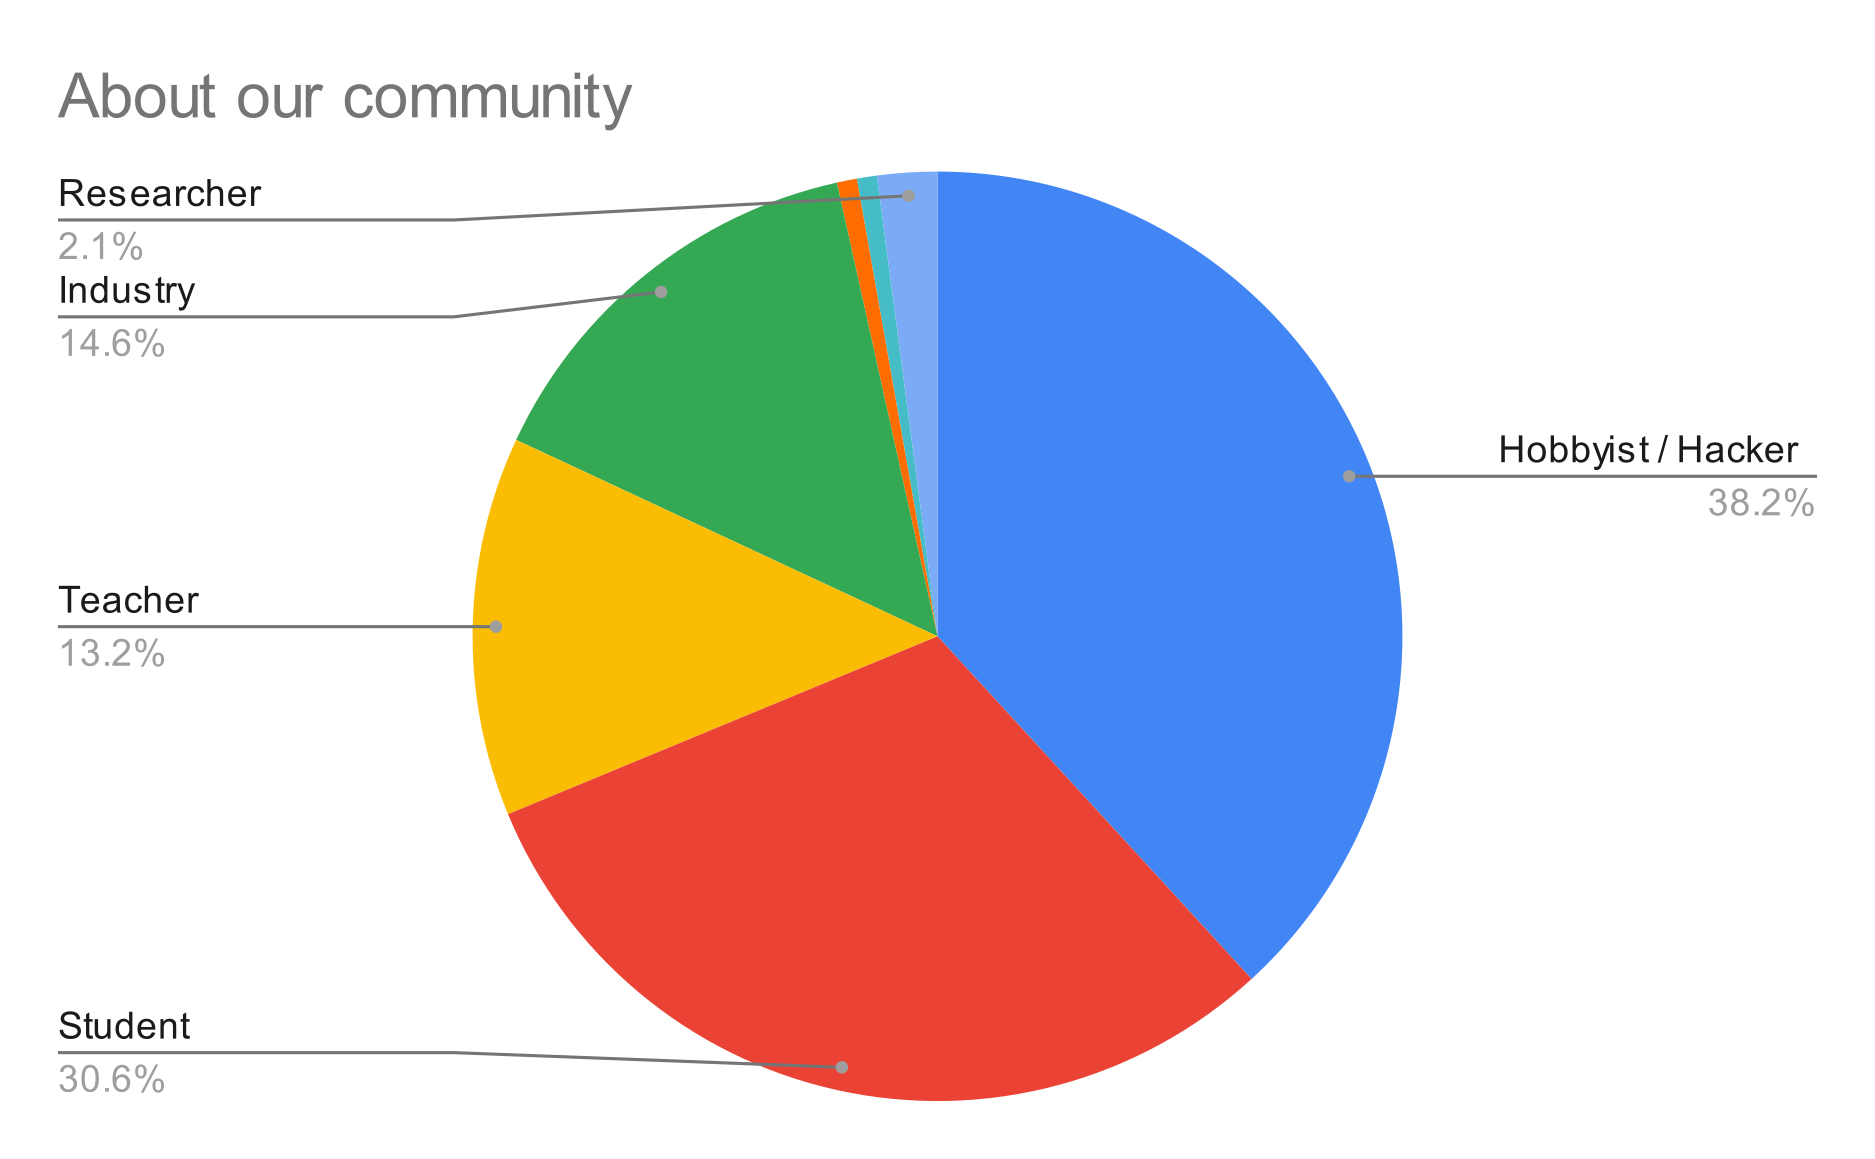
\includegraphics[width=\columnwidth]{./Figs/about our community pie chart.png}
\caption{Tiny Tapeout 4 participant self identification.}
\label{fig:TT04_submitters}
\end{figure}

The remainder of this paper will detail the Tiny Tapeout submission flow, multiplexer evolution, circuit board design, the results of post production silicon testing, and the project's next steps.

\begin{table*}[!t]
\centering
\caption{Tiny Tapeout shuttle summary}
\label{tab:tinytapeout}
\begin{tabularx}{\textwidth}{@{}l *{9}{X}@{}}
\toprule
\textbf{Run} & \textbf{Launched} & \textbf{Shuttle} & \textbf{Designs} & \textbf{Delivery date} & \textbf{Architecture} & \textbf{Number of IOs} & \textbf{IO bandwidth} & \textbf{Analog support} \\
\midrule
TT01 & 2022-08-17  & MPW7  & 152 & n/a        & Scan chain                & 16 & \qty{5}{\kHz}    & no  \\
TT02 & 2022-11-09  & 2211Q & 165 & 2024-01-30 & Scan chain                & 16 & \qty{5}{\kHz}    & no  \\
TT03 & 2023-03-01  & 2304C & 249 & 2024-02-28 & Scan chain inverted clock & 16 & \qty{10}{\kHz}    & no  \\
TT04 & 2023-07-01  & 2309  & 143 & 2024-04-15 & Mux                       & 26 & \qty{50}{\MHz}   & no  \\
TT05 & 2023-09-11  & 2311  & 174 & 2024-05-12 & Split Mux                 & 26 & \qty{50}{\MHz}   & no  \\
TT06 & 2024-02-01  & 2404  & TBD & 2024-11-30 & Split Mux                 & 38 & \qty{50}{\MHz}   & yes \\
\bottomrule
\end{tabularx}
\end{table*}

\begin{figure}[!t]
\centering
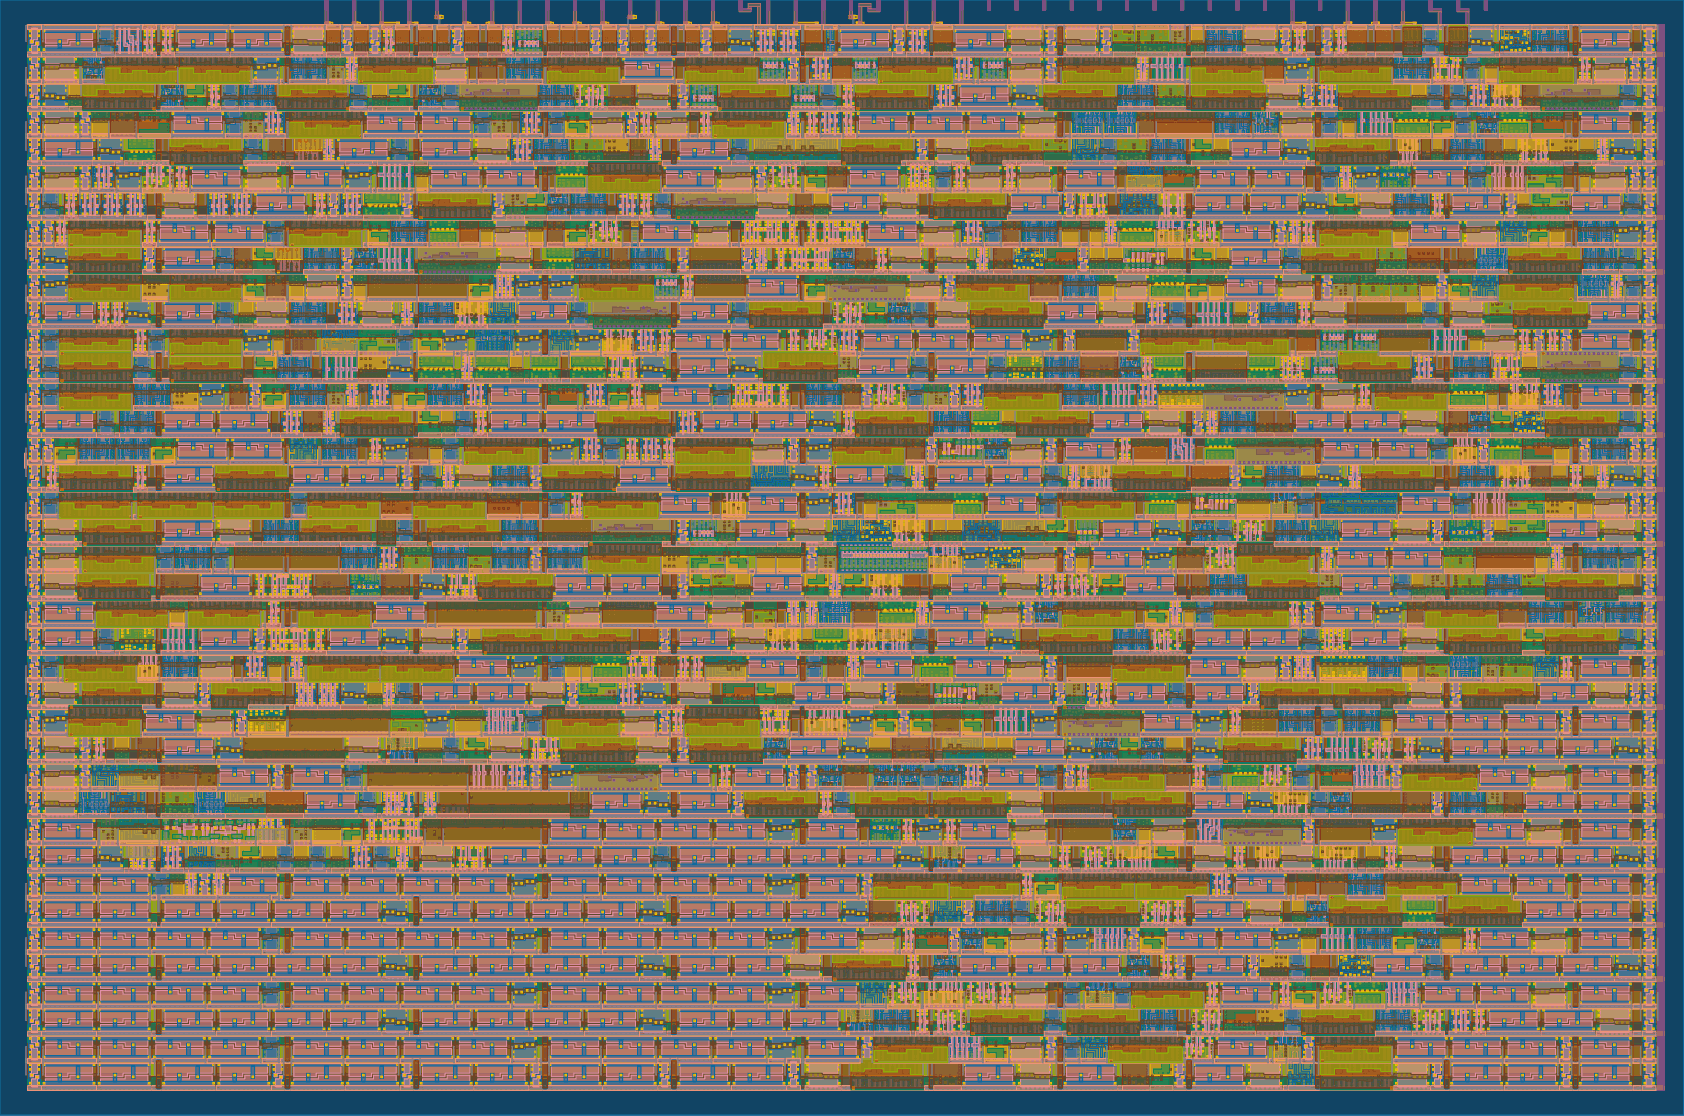
\includegraphics[width=\columnwidth]{./Figs/gh action gds layout.png}
\caption{A 2-D render of a single Tiny Tapeout tile.}
\label{fig:render_cells_in_use}
\end{figure}

\section{Submission Flow}
\label{sec:design_flow}

Tiny Tapeout designs are primarily developed in the Verilog hardware description language (HDL) or Wokwi~\cite{wokwi}
Wokwi is a web based visual schematic editor for hardware description, designed as an easier way for individuals with no prior HDL experience to get started.
The Tiny Tapeout website~\cite{tinytapeout} includes a basic getting started guide for Wokwi, demonstrating how to use the tool to draw circuits, which is made available in English and Spanish.

The process of designing an ASIC for submission to Tiny Tapeout, whether with Wokwi, Verilog, or another HDL, matches existing workflows built around the same tools and is outside the scope of this article; instead, we focus here on the aspects of the submission flow which differ from traditional ASIC design and production flows.

\begin{figure}[!t]
\centering
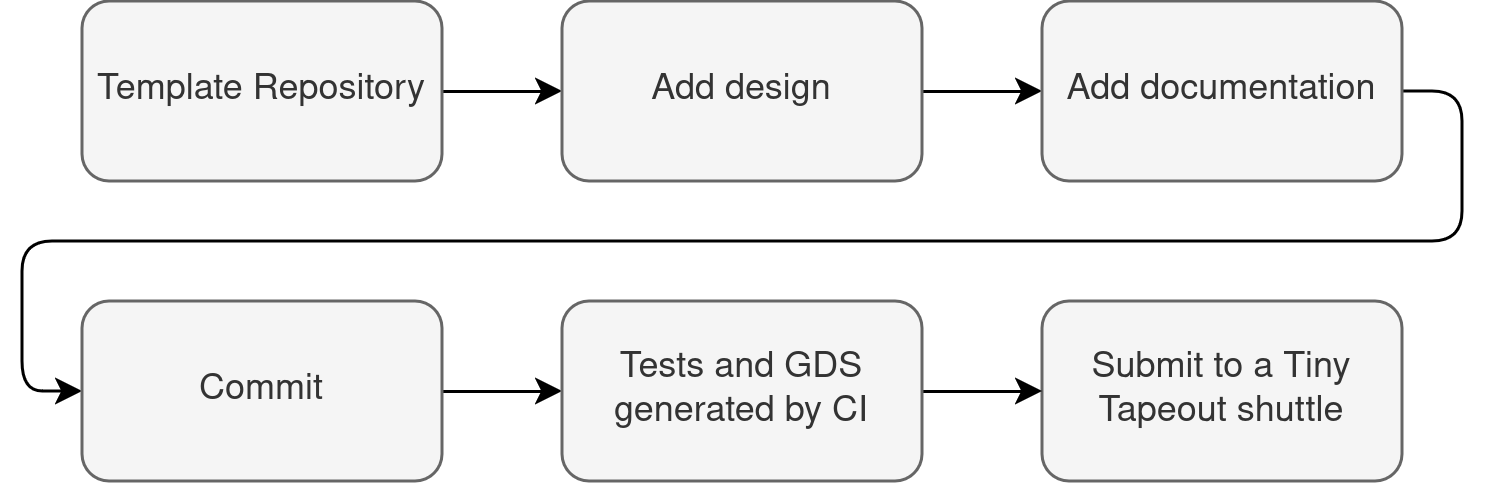
\includegraphics[width=\columnwidth]{./Figs/submission_flow.png}
\caption{Design Submission Flow}
\label{fig:submission_flow}
\end{figure}

The submission flow starts with the participant creating a GitHub~\cite{github} source code repository from a template provided by Tiny Tapeout. Using this template and guidance provided through the Tiny Tapeout website and broader communication channels the participant then creates their chip design in Verilog, Wokwi, or the HDL of their choice.

The participant's design must then be documented, after which the design and its documentation can be commited and pushed to the GitHub repository. This submission triggers automated tests and the generation of binary layout files in GDSII~\cite{gds} format.

This automated testing and GDS generation is handled through the Tiny Tapeout GitHub templates\cite{verilogtemplate} using GitHub Actions\cite{githubactions}---an automatic continuous integration system triggered every time the repository is updated. This reduces duplicated effort and makes it possible for Tiny Tapeout to support large numbers of participants without excessive technical overhead.

There are four main jobs in the continuous integration system:

\begin{enumerate}
	\item GDS: installs OpenLane\cite{openlane} and the SkyWater Sky130\cite{skywaterpdk} PDK, builds the binary layout files, and generates a summary of the design (Fig.~\ref{fig:summary_table_GDS_job}). The summary includes utilization, standard cells used, a 2-D render (Fig.~\ref{fig:render_cells_in_use}) and an interactive 3-D viewer (Fig.~\ref{fig:interactive_3D_viewer}).
This job can also optionally run a gate-level verification of the design.
	\item Verification: installs the YosysHQ open source computer-aided design (CAD) suite, which includes many common electronic design automation (EDA) tools; uses iVerilog\cite{iverilog} and cocotb\cite{cocotb} to run any included testbenches.
	\item Documentation: generates a preview of the documentation.
	\item Precheck: runs design rule check (DRC) tests to ensure the design can be integrated into the multi project chip.
\end{enumerate}

Successful GDS, Documentation, and Precheck job completion are all required for a design to be submitted to a shuttle for production.
Verification is optional but highly encouraged. Submissions designed in Wokwi are able to make use of its integrated truth table testing system\cite{automatedtesting}.

If all tests pass and the binary layout files are correctly generated the design can then be submitted to a quarterly shuttle for production in silicon, alongside all other passing designs from participants in that Tiny Tapeout run. Projects are submitted to a shuttle through the Tiny Tapeout website~\cite{tinytapeout}. Participants are free to update submitted projects up until the closing date of the shuttle, providing the tests continue to pass.

While the Tiny Tapeout continuous integration system can be run entirely in the user's web browser, it is also possible to install a local copy of the tools\cite{localinstall} on a participant's computer. Locally installed tools can help to reduce the time between design iterations, especially for the test and verification jobs.

With its focus on automated testing Tiny Tapeout is able to minimize design errors common to those coming to ASIC design with little or nor prior experience, reducing wastage at the production stage and maximizing

\begin{figure}[!t]
\centering
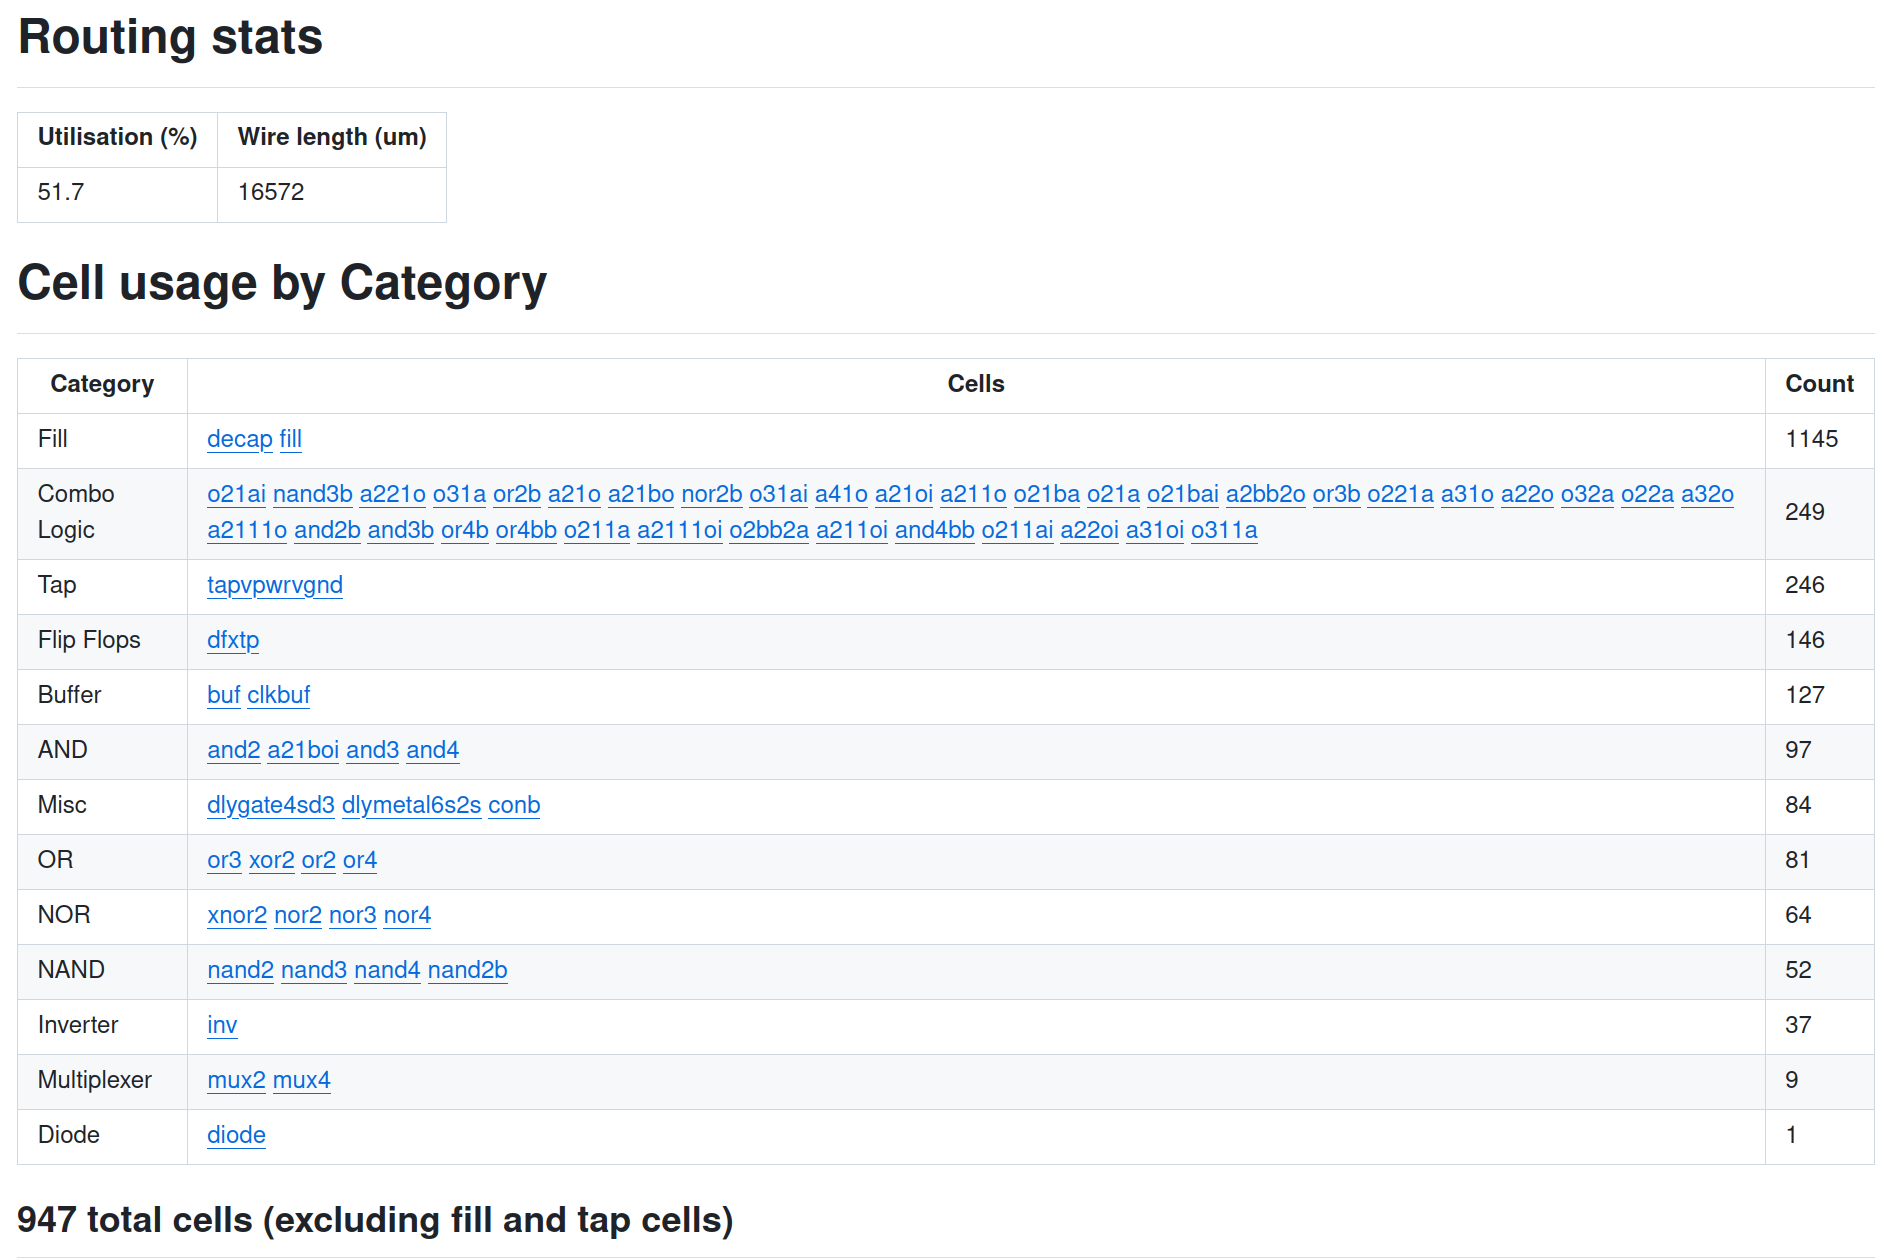
\includegraphics[width=\columnwidth]{./Figs/gh action cell stats.png}
\caption{A summary table from the GDS continuous integration job.}
\label{fig:summary_table_GDS_job}
\end{figure}

\begin{figure}[!t]
\centering
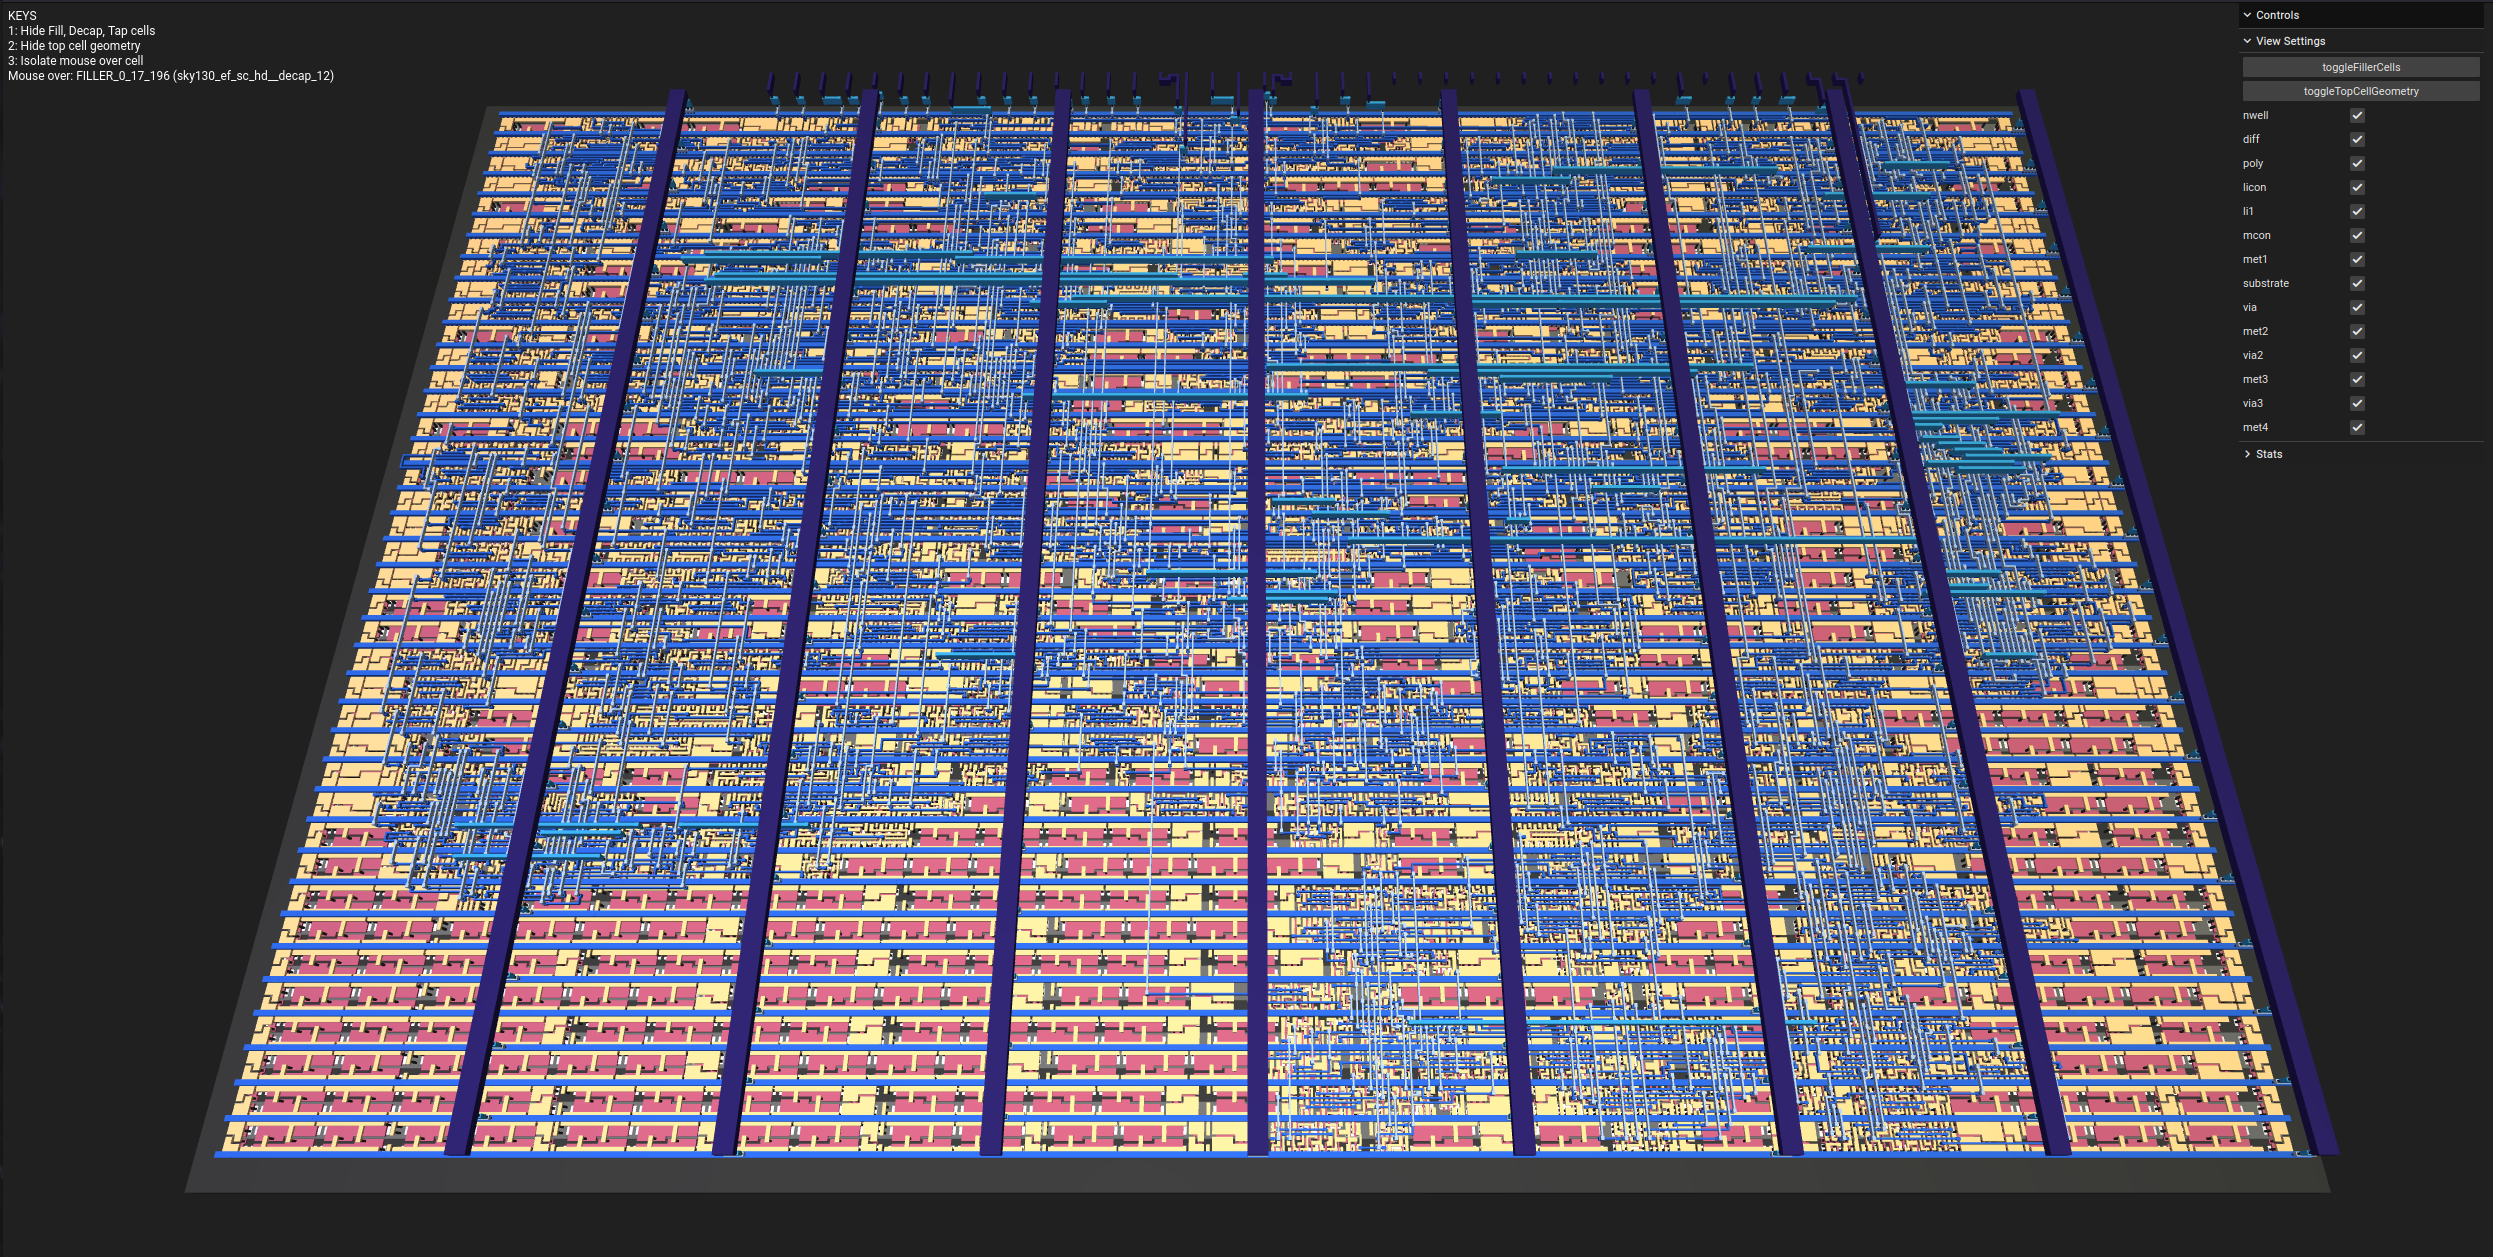
\includegraphics[width=\columnwidth]{./Figs/gh action gds 3d view.png}
\caption{The interactive 3-D viewer.}
\label{fig:interactive_3D_viewer}
\end{figure}

\section{Tiny Tapeout 1}
\label{sec:tinytapeout1}

The Tiny Tapeout project started as an experiment in fitting as many designs as possible into the \qty{10}{\milli\meter\squared} available on the Google lottery shuttles (Fig.~\ref{fig:500_designs_chain_TT01}) using the Efabless Caravel harness.
In order to prove the concept as rapidly as possible initial designs were based on a scan chain architecture to simplify testing.

Each Tiny Tapeout 1 design has eight inputs and eight outputs.
Clock and reset signals were optional and not treated specially. The chain was formed of scan flops~\cite{skywaterpdk}, a type of flip flop with a multiplexer integrated at its input. An example showing a two design scan chain is shown in Fig.~\ref{fig:simplified_view_2_designs}.

\begin{figure}[!t]
\centering
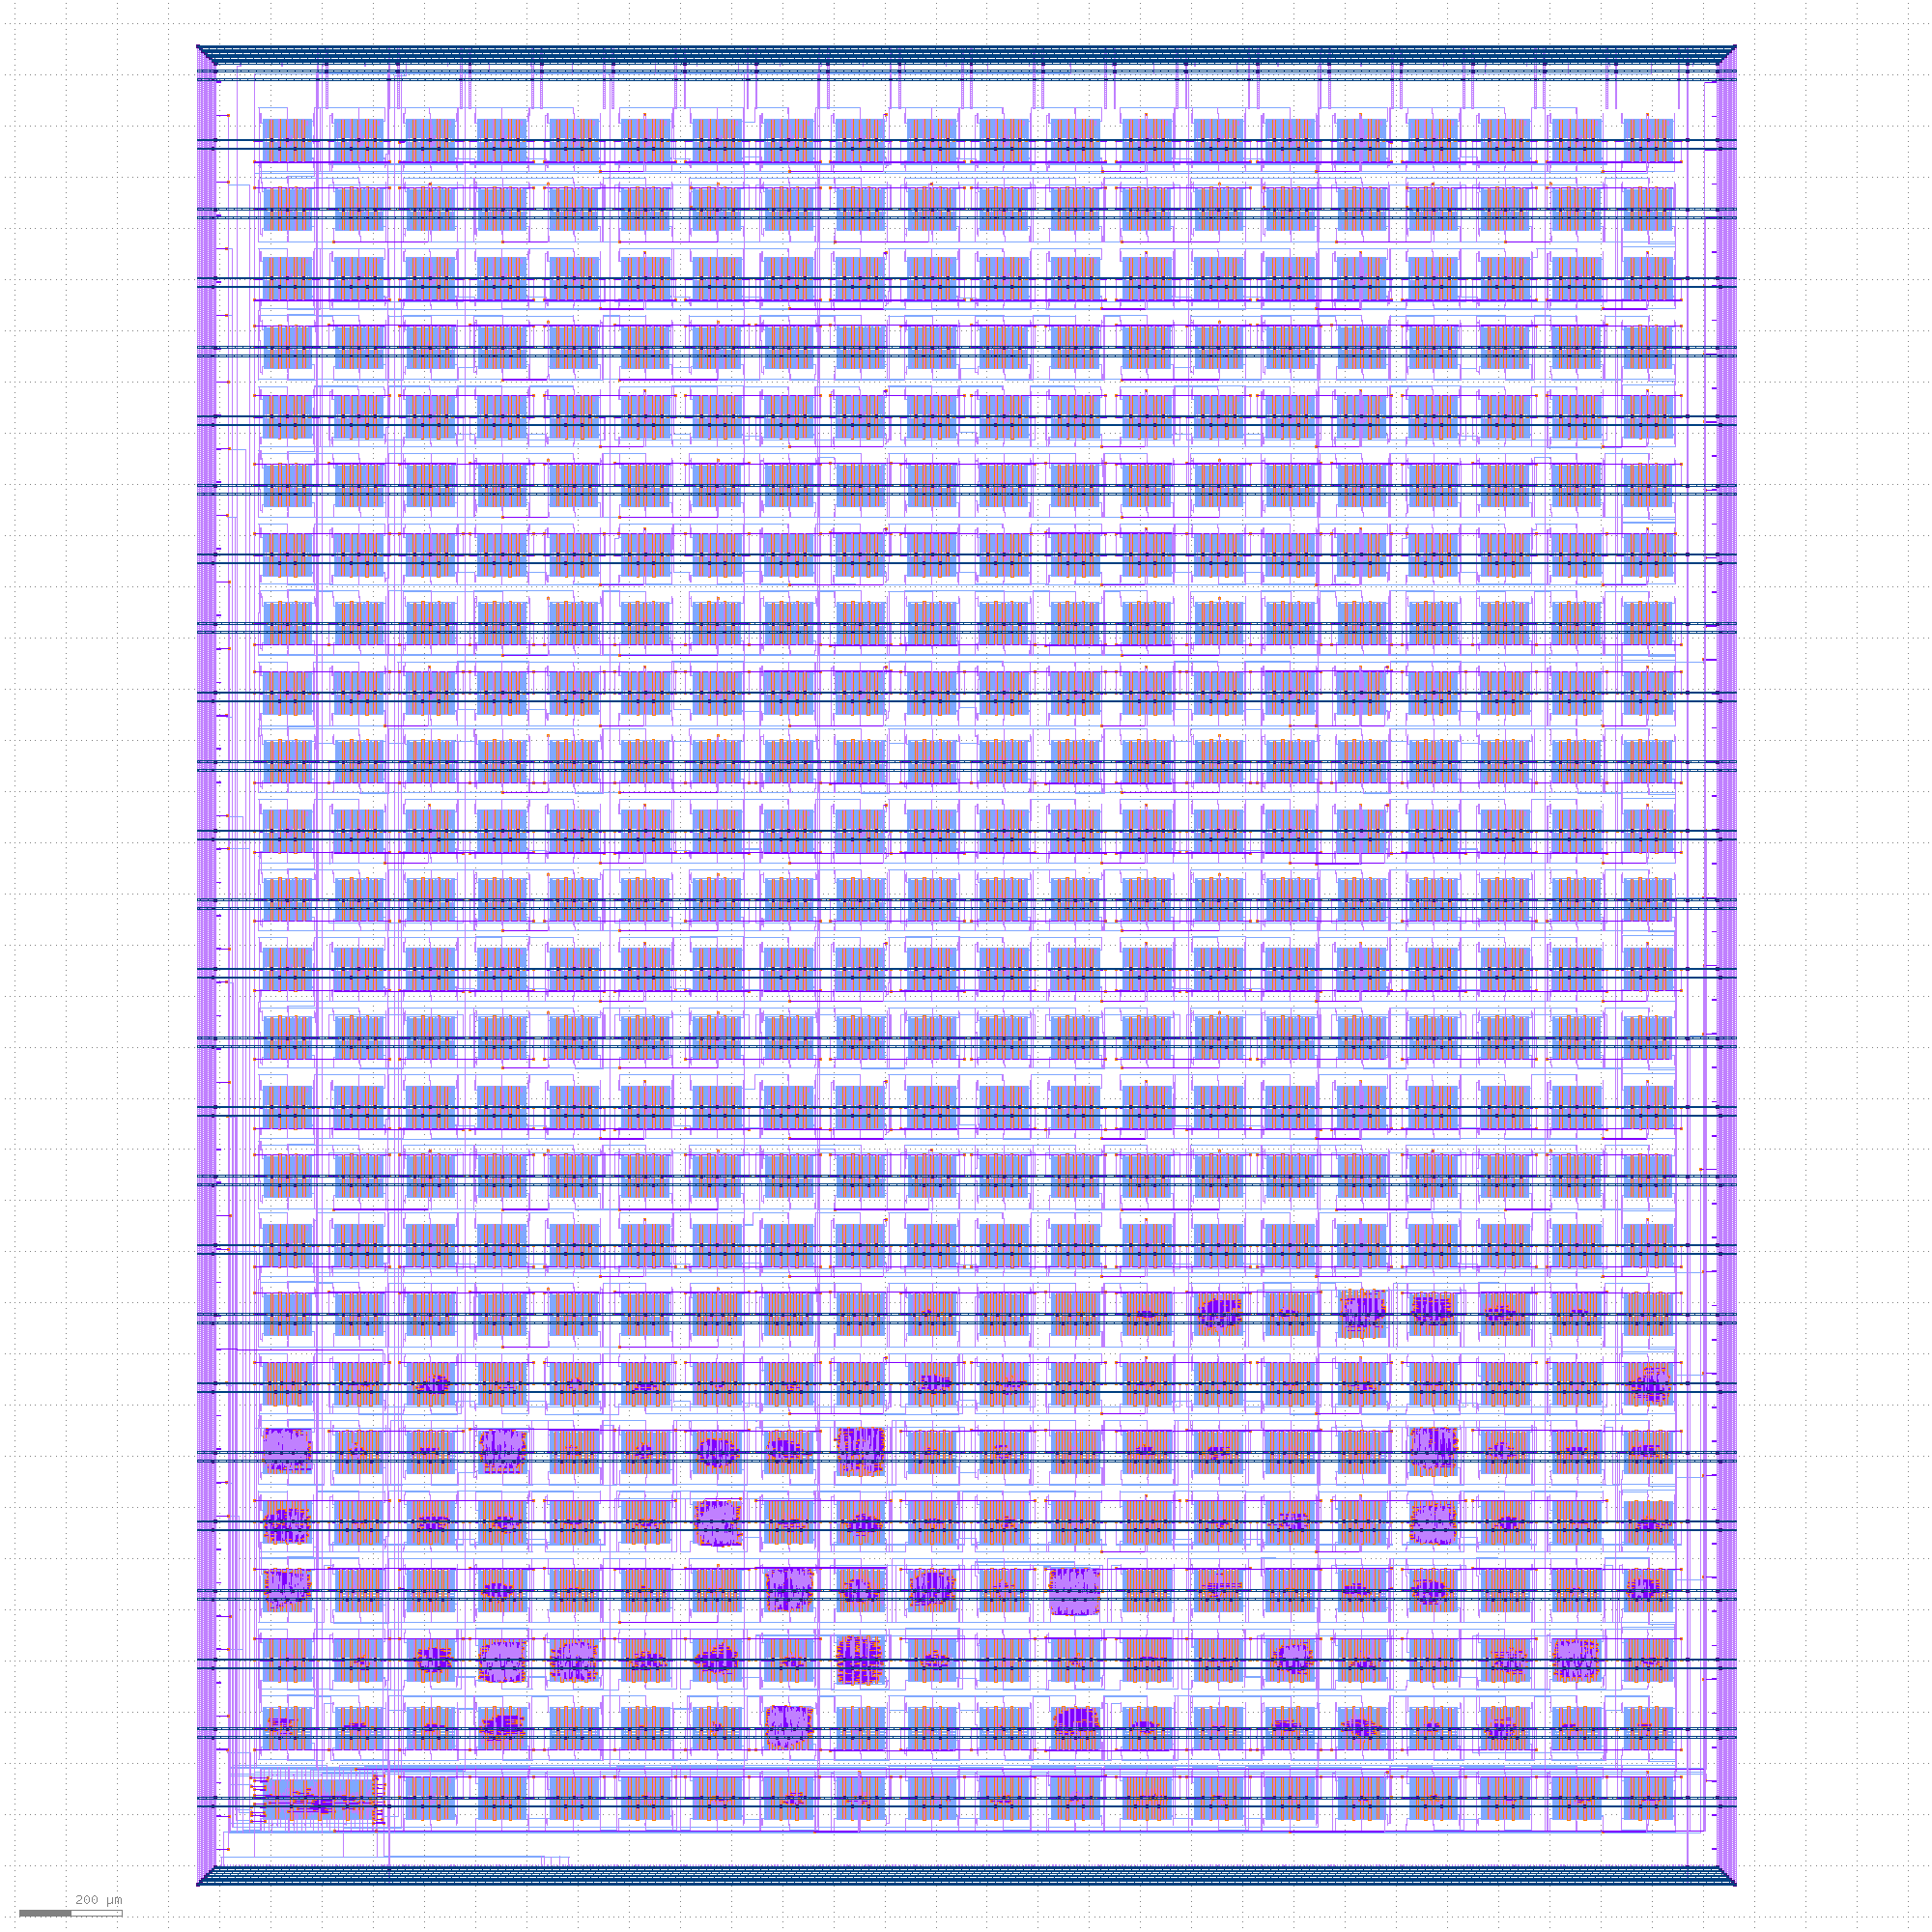
\includegraphics[width=1\columnwidth]{./Figs/tt01_whole_die.png}
\caption{500 designs connected in a chain for Tiny Tapeout 1; the scan chain driver can be seen in the lower left corner.}
\label{fig:500_designs_chain_TT01}
\end{figure}

\begin{figure}[!t]
\centering
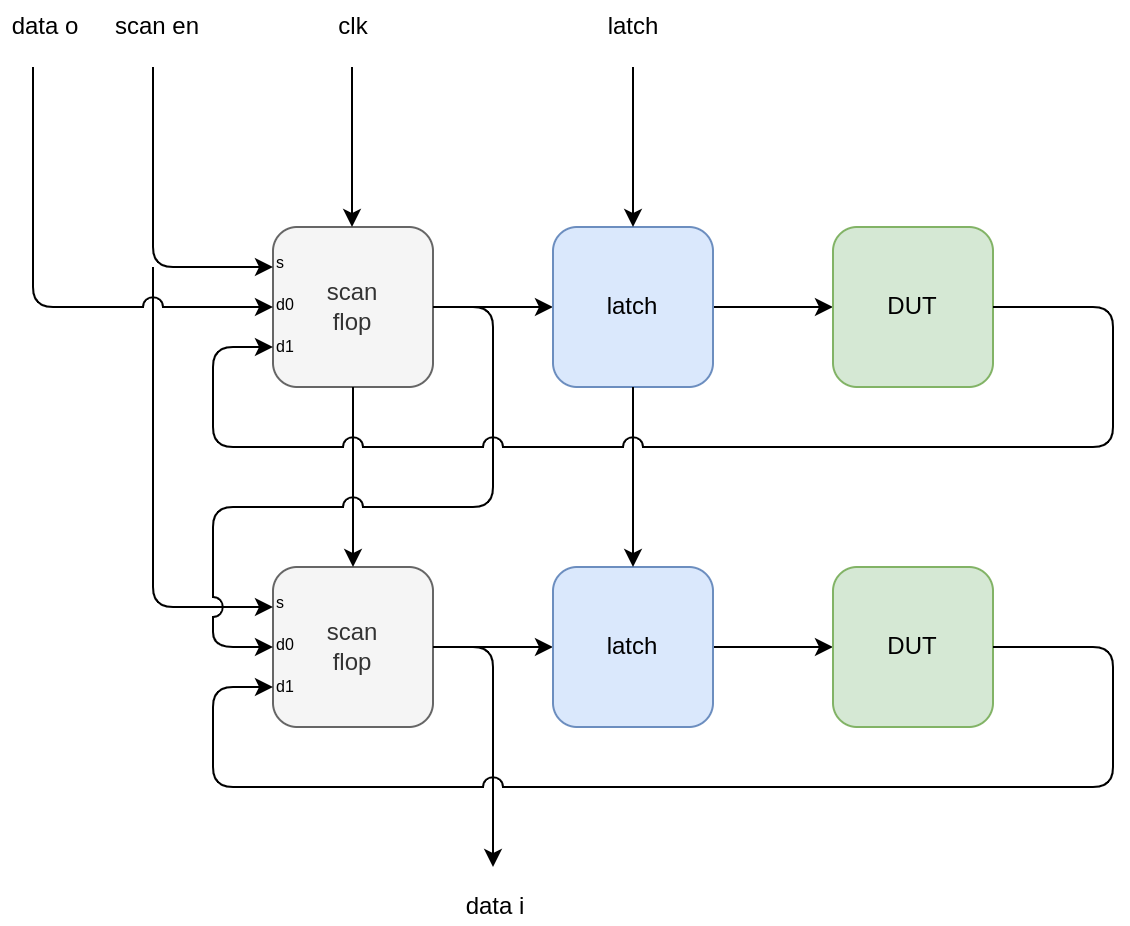
\includegraphics[width=\columnwidth]{./Figs/scanchain_block_diagram.png}
\caption{A simplified view of two Tiny Tapeout 1 designs in the scan chain.}
\label{fig:simplified_view_2_designs}
\end{figure}

Each design sends data into the secondary input of the scan flop and receives its own input from the output of the flop via a latch.
The chain is built~\cite{updateiodesign} by sending data from the output of the previous scan flop into the primary input of the next scan flop.
This arrangement allows the loading of data into any of the designs, followed by the capturing of the output and its clocking through the rest of the chain to the overall chain output.

While relatively easy to implement, a scan chain architecture has a downside: high latency.
As more designs are added to the chain it takes longer to send and receive data through it.
For example: assuming a \qty{50}{\MHz} scan chain clock with \qty{250} designs each having eight inputs and eight outputs, the maximum refresh rate of the resulting chain is $\qty{50}{\MHz} / (8 \times 250) = \qty{25}{\kHz}$.

The Tiny Tapeout 1 scan chain was embedded into each design, meaning a user could unintentionally remove it and break the chain.
This risk was mitigated with a formal equivalence check~\cite{tinytapeoutscan} which proves the chain was present in each submitted design and prevents submission if it has been removed.

Another concern with the scan chain design was hold violations, due to the large number of serially connected flops and potentially large clock skews over long signal wires. This was mitigated by reclocking the output data with a negative edge (negedge) flop, providing substantially more hold margin.

Following static timing analysis (STA) it was discovered that the clock duty cycle could change substantially due to the \qty{500} sequential clock drivers in the chain. Depending on the clock buffers and capacitance between each design the clock duty cycle could either increase or decrease, with this effect accumulated over the chain.

The verification effort~\cite{verificationmd} for the scan chain was broad and included a community review, register transfer level (RTL) and gate level (GL) simulation, formal verification\cite{sby}, STA, layout vs. schematic (LVS), DRC, and device level static verification~\cite{cvc}.

\section{Tiny Tapeout 2}
\label{sec:tinytapeout2}

\begin{figure}[!t]
\centering
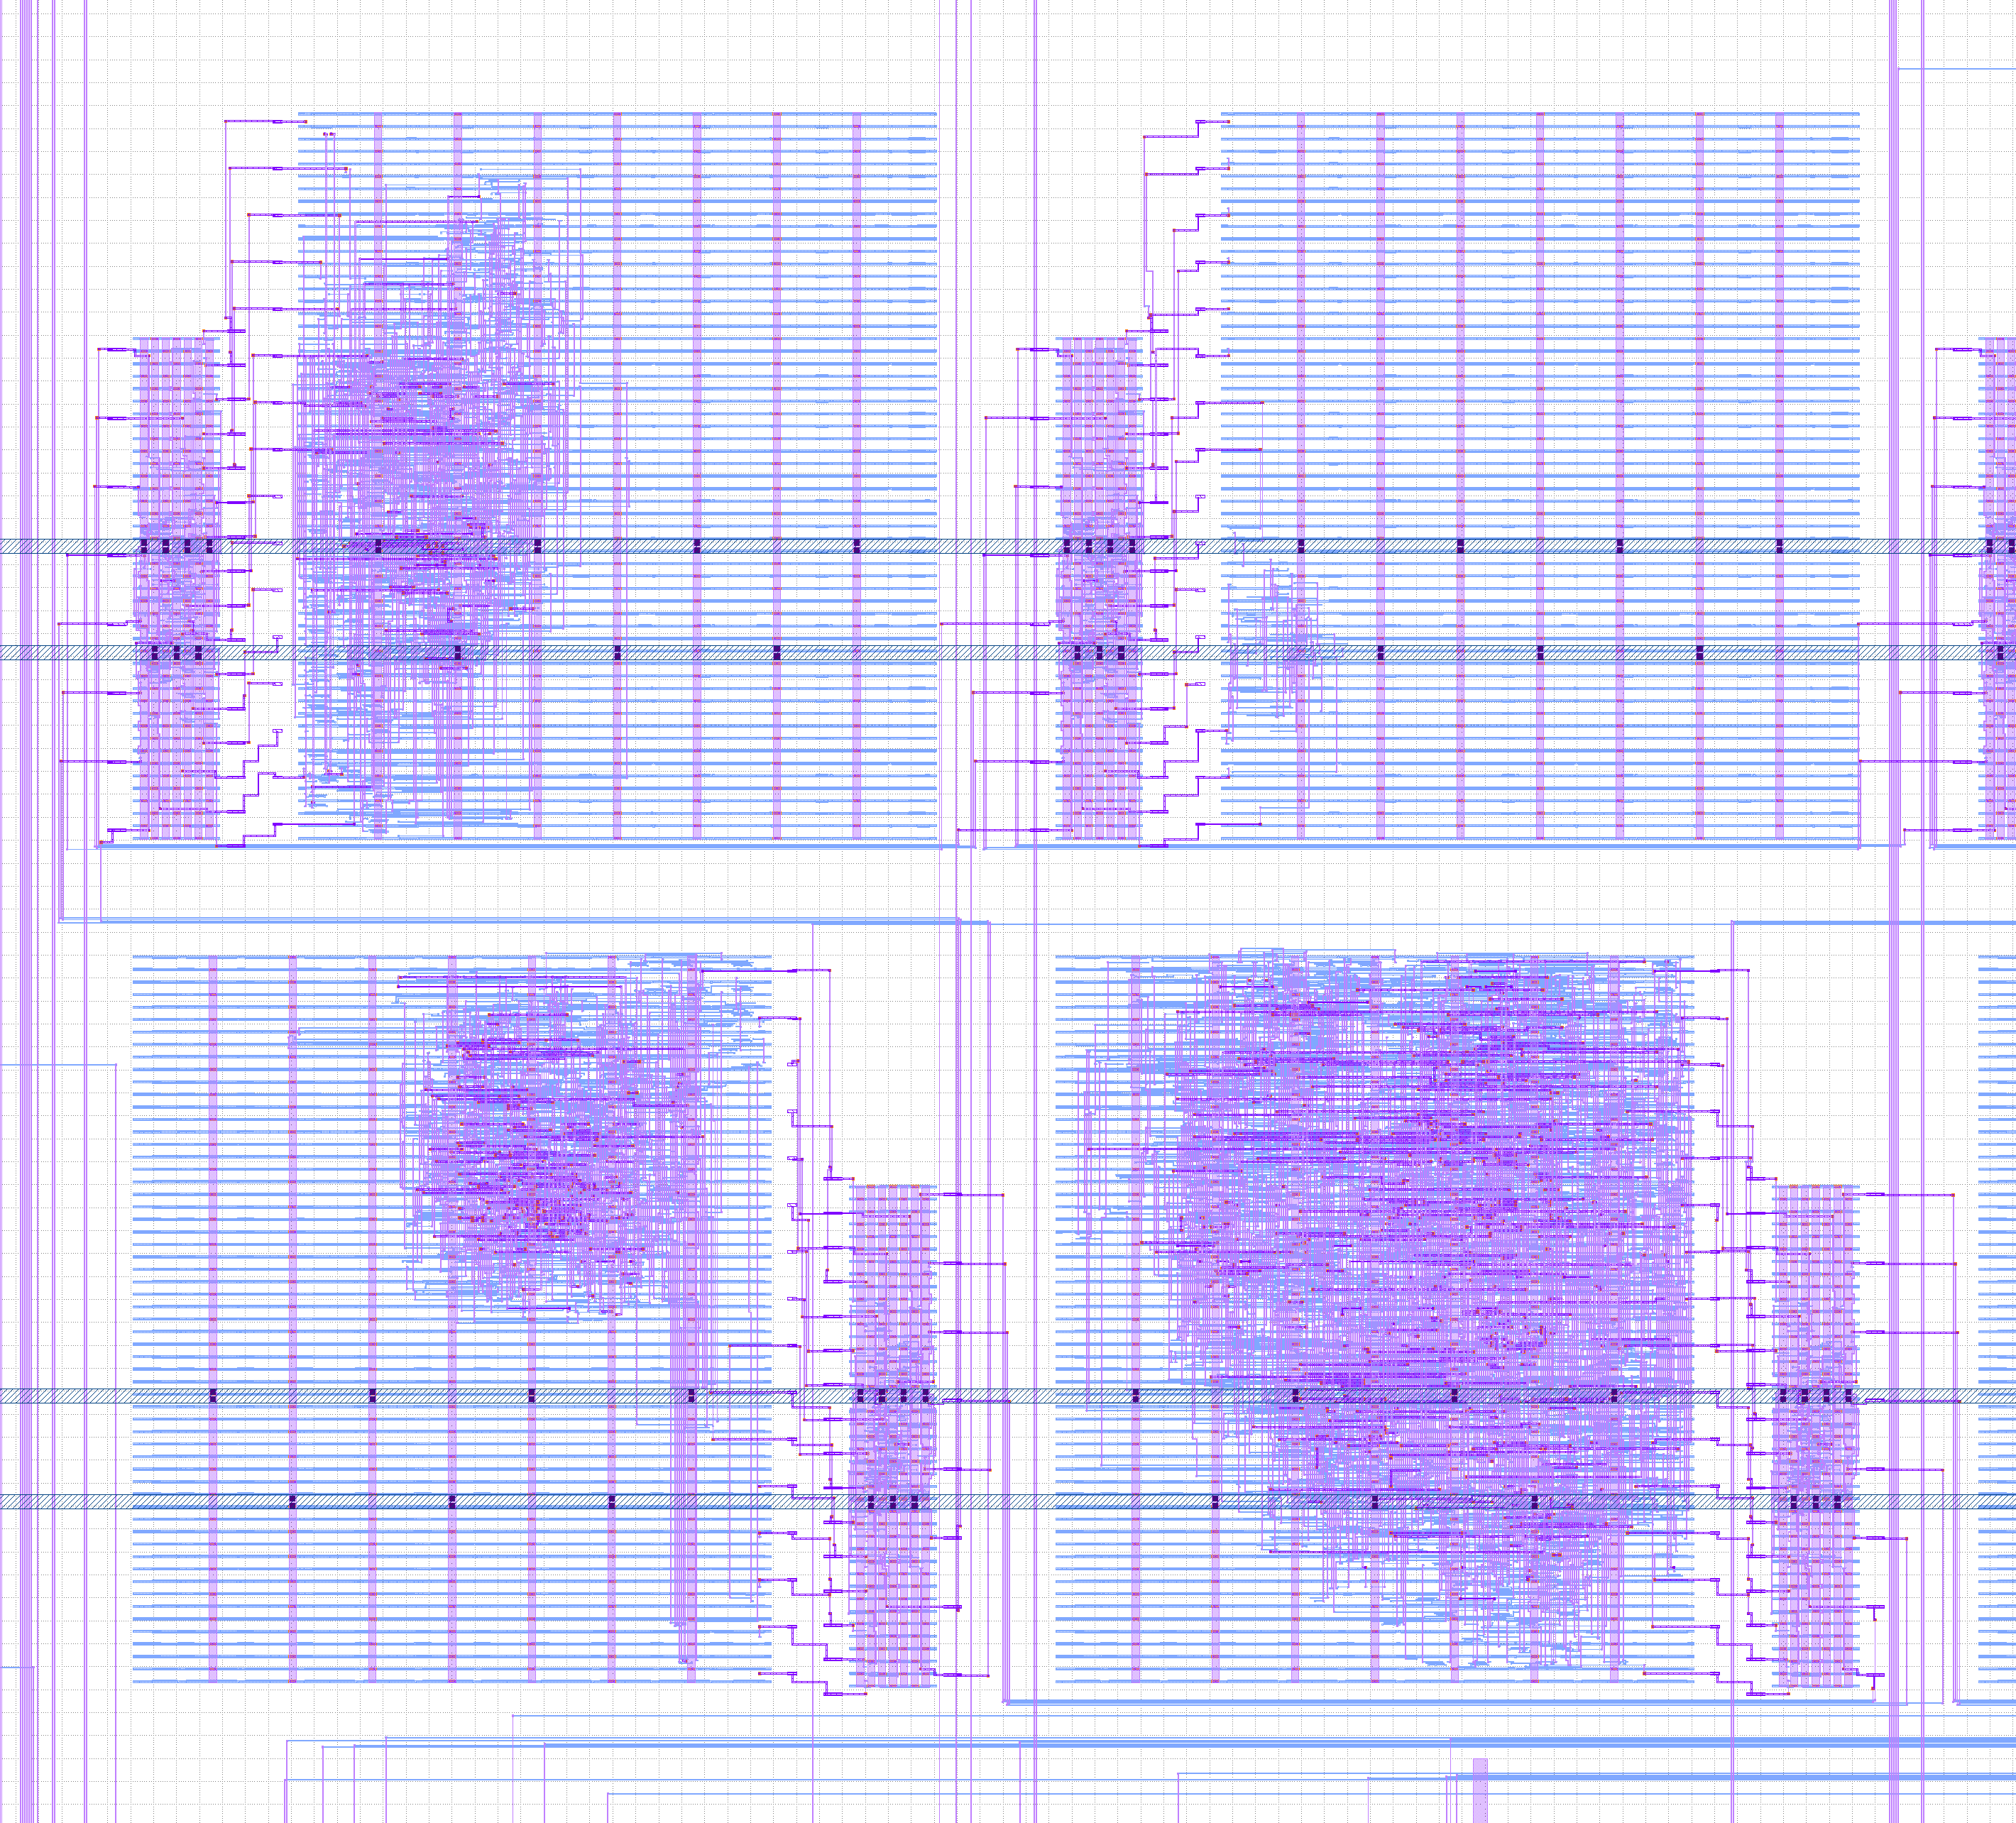
\includegraphics[width=\columnwidth]{./Figs/tt02_gds_zoom.png}
\caption{Tiny Tapeout 2 designs, showing the discrete scan chain blocks.}
\label{fig:TT02_separate_scan_blocks}
\end{figure}

After the concept had been proven, Tiny Tapeout 2 opened in November 2022 and \qty{165} designs were submitted. For this run participants were charged a fee and silicon manufacture was guaranteed. This was a big step forward for small scale ASIC production, as until that time the only way to get guaranteed silicon with the open source PDKs was to pay for a full chipIgnite slot, costing {\$}\qty{10,000}. The finished design was submitted for fabrication on Efabless chipIgnite 2211Q.

To address the issue of accidental macro block removal encountered in Tiny Tapeout 1, Tiny Tapeout 2 moved the scan chain into a discrete macro block~\ref{fig:TT02_separate_scan_blocks}. This was present in all designs, and could not be modified by participants.

As with Tiny Tapeout 1, designs in in Tiny Tapeout 2 used two clock buffers, with the internal flops driven after the first buffer.

Tiny Tapeout 2 silicon was received in October 2023, tested for the first time on a public livestream, mounted on PCBs, and sent to participants in January 2024.

\section{Tiny Tapeout 3}
\label{sec:tinytapeout3}

Tiny Tapeout 3 opened in March 2023 and \qty{100} new designs were submitted by participants. To fill the remaining space an additional \qty{149} designs were added from TT01.

For Tiny Tapeout 3 the two clock buffers of Tiny Tapeout 1 and 2 were replaced by an inverting clock buffer design, with only one buffer between the clock input and output. Fig. ~\ref{fig:TT02_vs_TT03} shows a comparison between the TT02 and TT03 clock buffer designs. By inverting the clock between each design any asymmetry in the clock pulse is evenly spread across the negative and positive cycles.

\begin{figure}[!t]
\centering
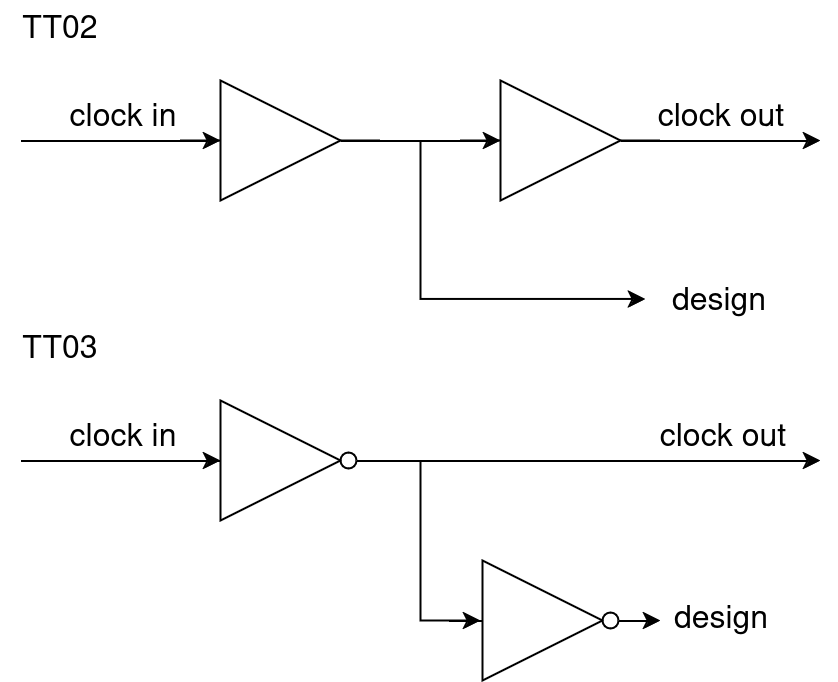
\includegraphics[width=\columnwidth]{./Figs/tt02 vs tt03 scanchain clock.png}
\caption{The Tiny Tapeout 3 architecture buffers the output from the clock network into each design. Clock polarity is alternated between designs to minimize asymmetry between positive and negative cycles.}
\label{fig:TT02_vs_TT03}
\end{figure}

Silicon was received in January 2024, and at the time of writing was being assembled for delivery to customers by March 2024.

Following the closure of Tiny Tapeout 3 an invitational experimental shuttle dubbed Tiny Tapeout 3.5 ~\cite{tinytapeout03p5} was submitted for production. This featured \qty{32} designs, each testing and previewing some of the changes planned for Tiny Tapeout 4 as detailed in the next section. Two of these designs included a power gate, as a stepping stone to supporting analog and mixed signal designs.

The finished design was submitted for production on Efabless chipIgnite 2306C.
Silicon was received in December 2023 and at the time of writing was being assembled for testing.

\section{Tiny Tapeout 4}
\label{sec:tinytapeout4}

The biggest limitations of the scan chain based architecture used in Tiny Tapeout 1 through 3 inclusive were its limited IO bandwidth and high latency.
It was decided that a new architecture was needed for Tiny Tapeout 4 and proposals were gathered from the community.
An online video call was held with community members, and the ten submitted architecture proposals discussed.

The winning architecture was a straightforward multiplexer design, shown in Fig.~\ref{fig:multiplexer_design}. This architecture was chosen as the simplest to implement while providing the most benefit in terms of additional IOs and higher bandwidth.

\begin{figure}[!t]
\centering
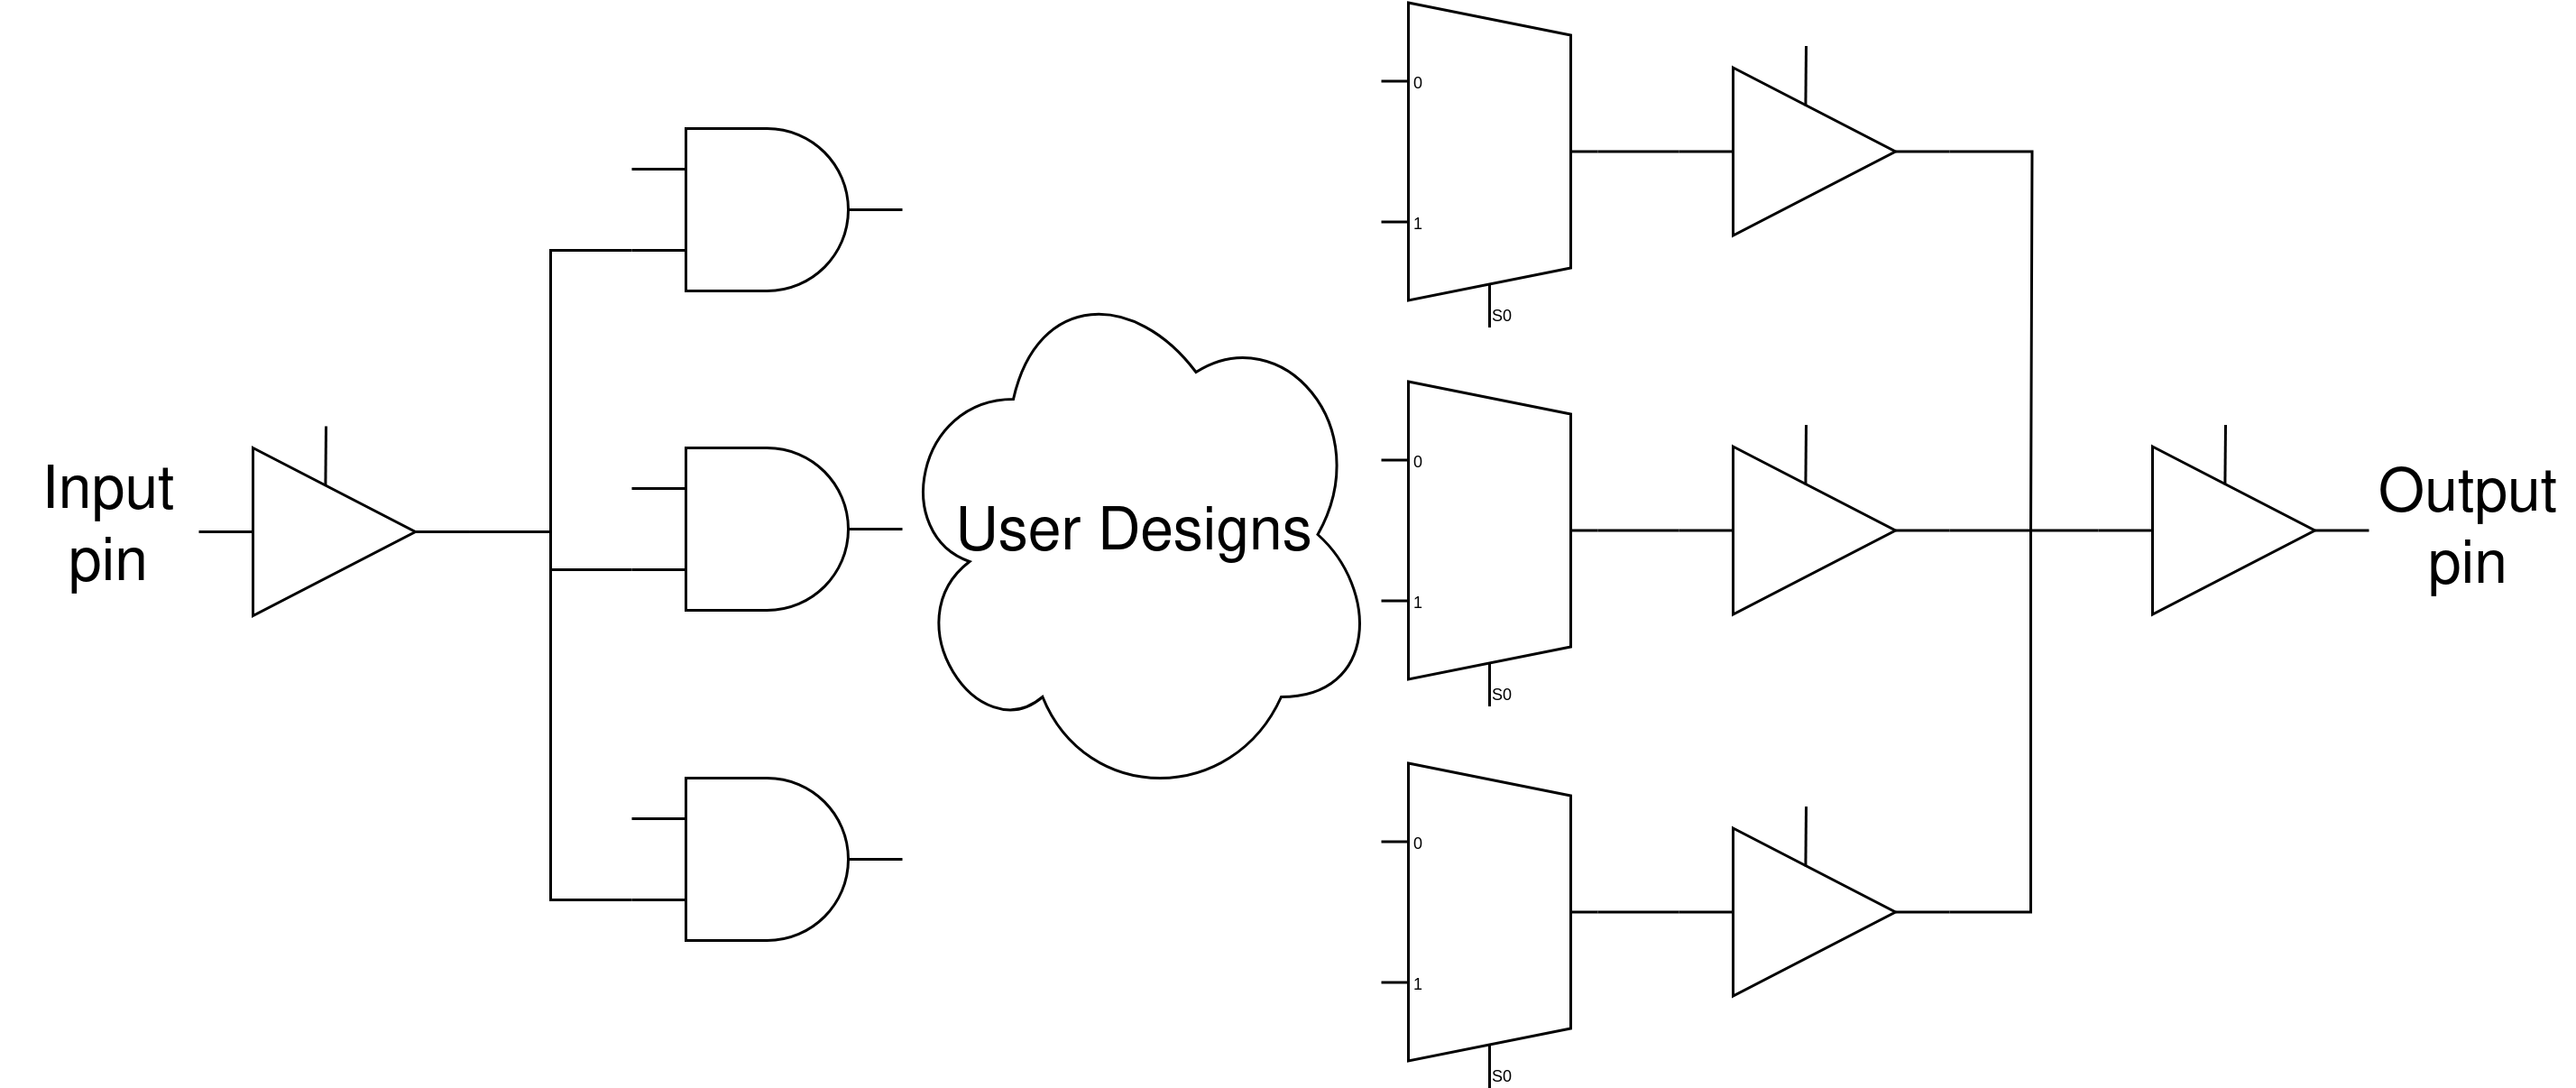
\includegraphics[width=\columnwidth]{./Figs/mux architecture.png}
\caption{A simplified diagram of the Tiny Tapeout 4 multiplexer architecture.}
\label{fig:multiplexer_design}
\end{figure}

The physical layout tested in Tiny Tapeout 3.5 and finalized in Tiny Tapeout 4 (shown in Fig.~\ref{fig:TT03_5_test_design}) consists of a central controller connected up and down to two vertical wiring spines.
For this experimental run we also included loopback test designs at the end of each multiplexer so we could measure performance for each multiplexer position.

Twenty-four horizontal multiplexers connect to the wiring spines, each of which supports 16 designs.
This allows for up to 384 separate single tile designs.
The new architecture also enabled multiple tile designs, allowing a maximum project size of $8 \times 2$ tiles or $1359 \times \qty{225}{\um\squared}$---around \num{20000} logic cells. Table~\ref{tab:comparison_TT03_TT04} shows the key differences between Tiny Tapeout 3 and Tiny Tapeout 4.

\begin{figure}[!t]
\centering
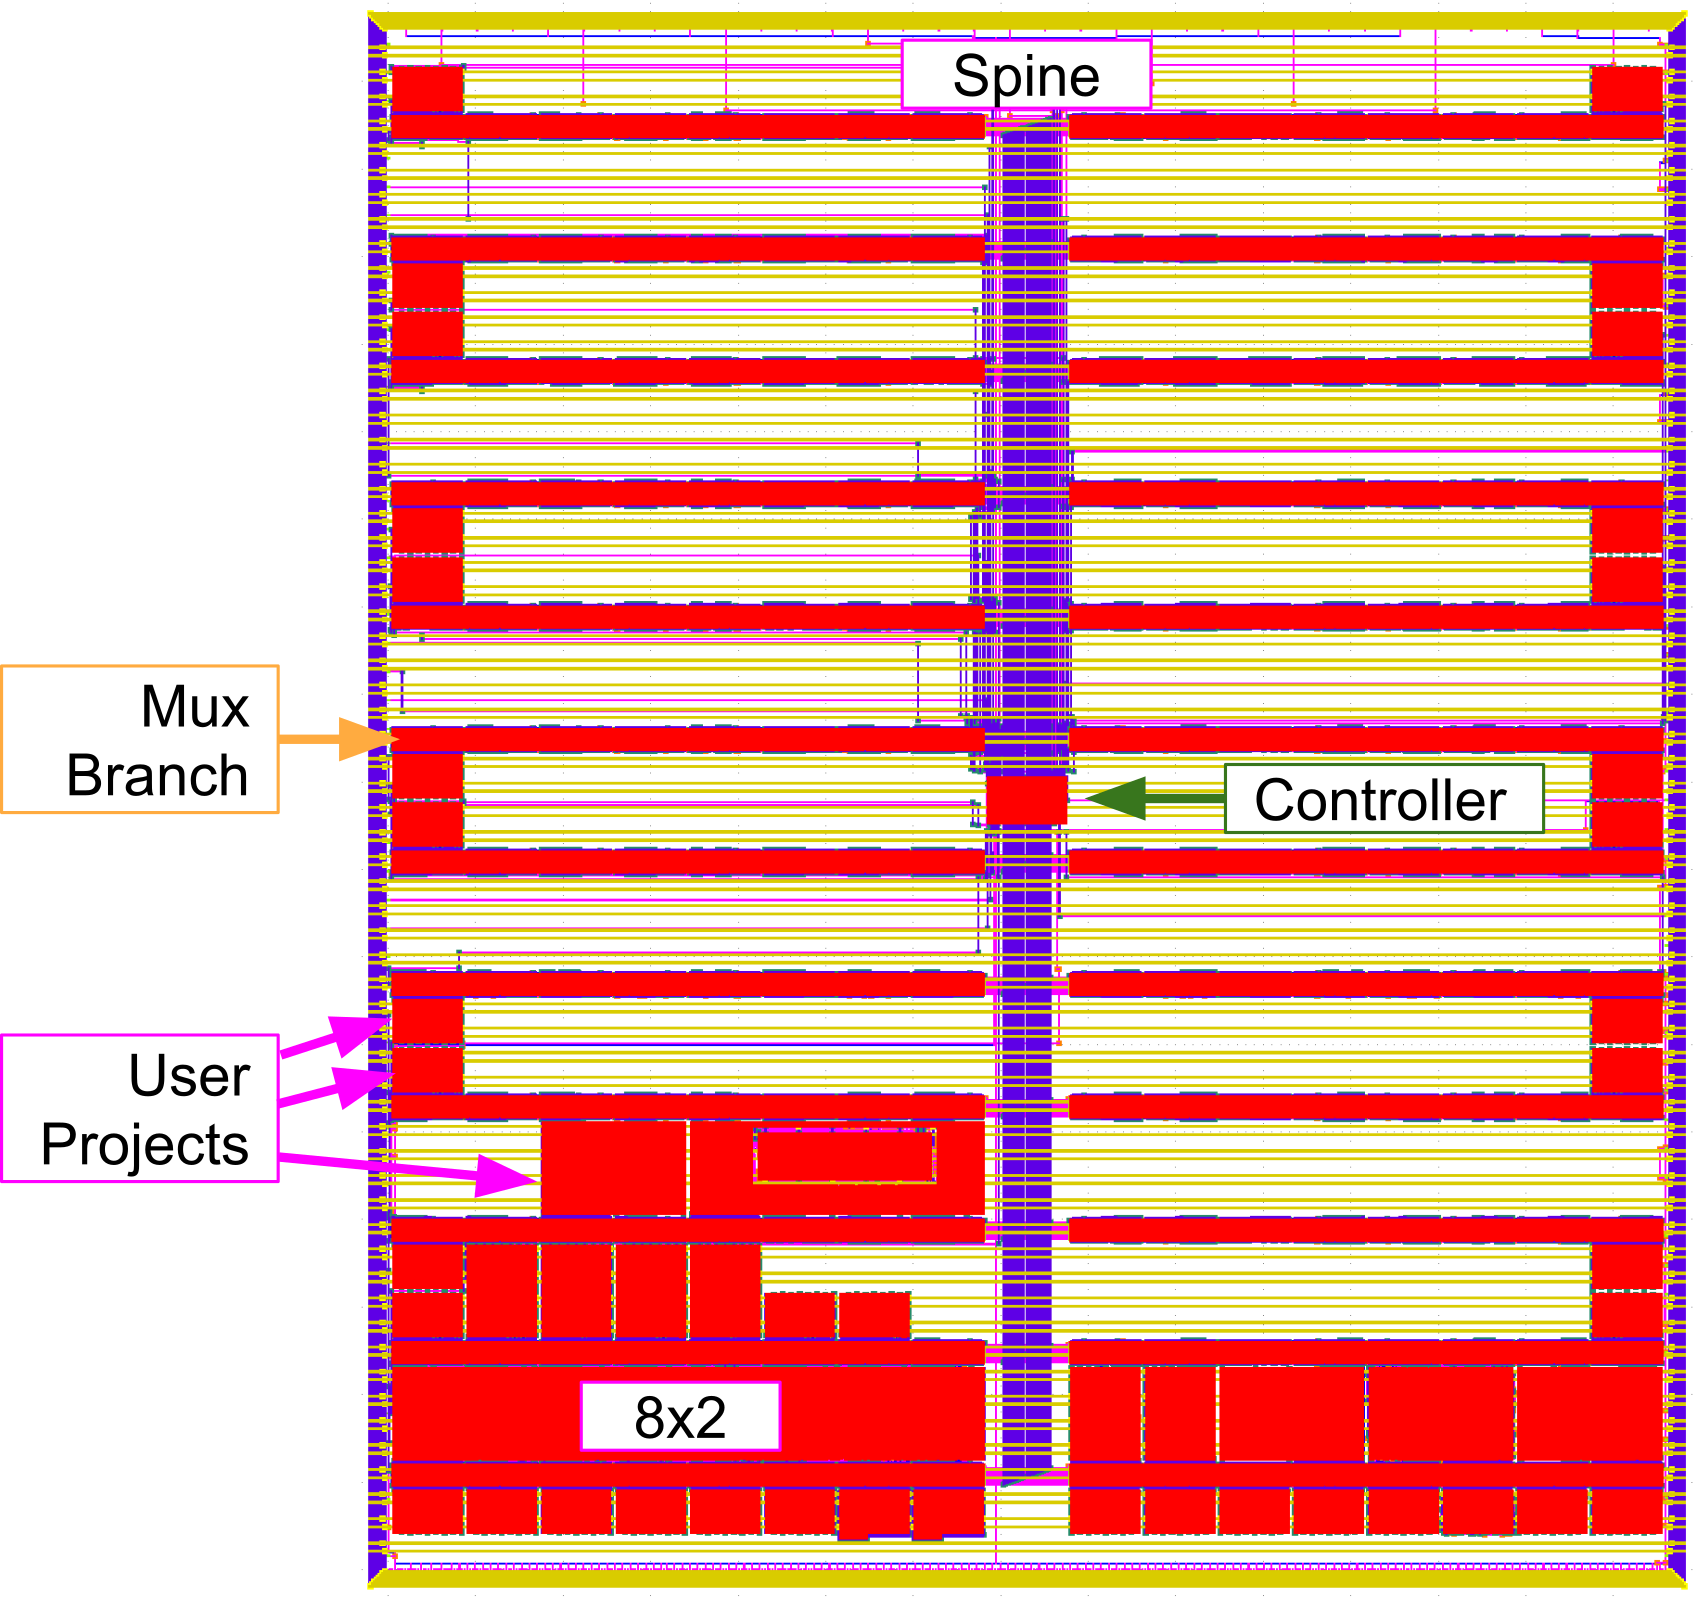
\includegraphics[width=\columnwidth]{./Figs/tt3p5 layout.png}
\caption{The Tiny Tapeout 3.5 test design.}
\label{fig:TT03_5_test_design}
\end{figure}

Another major limitation of the scan chain architecture used in Tiny Tapeout 1 through Tiny Tapeout 3 was the small number of IO pins.
The scan controller used nine GPIOs to select the currently active design. While this simplified the demonstration board board, it also wasted valuable IO pins.

Starting with Tiny Tapeout 4 the parallel design selection architecture used in previous chips was dropped in favor of a serial protocol.
The extra pins thus provided were then used bidirectionally, giving each design a clock pin, reset pin, and 24 IO pins.

\begin{table}[!t]
\centering
\caption{A comparison between Tiny Tapeout 3 and Tiny Tapeout 4.}
\label{tab:comparison_TT03_TT04}
\begin{tabular}{@{}lcc@{}}
\toprule
Parameters & TT03 & TT04 \\
\midrule
Max clock speed & \qty{8}{\kHz} & \qty{50}{\MHz} \\
Max design size & $150 \times \qty{170}{\um\squared}$ & $1359 \times \qty{225}{\um\squared}$ \\
Input pins & 8 & 10 \\
Output pins & 8 & 8 \\
Bidirectional IO pins & None & 8 \\
Custom GDS file & \xmark & \checkmark \\
\bottomrule
\end{tabular}
\end{table}

\section{Tiny Tapeout 5}
\label{sec:tinytapeout5}

Tiny Tapeout 5 saw another change in the design, which split the multiplexer into two parts in order to improve performance. As a result of the split the controller was also updated to multiplex between the two halves.
Some other small changes to the multiplexer in Tiny Tapeout 5 included the tweaking, addition, or removal of buffers to improve the STA results.

As each spine segment in Tiny Tapeout 5 is now half as long as in Tiny Tapeout 4, it will exhibit half the capacitance. As a result, upon receipt and testing of fabricated chips, we expect to see the round trip latency reduced to around \qty{10}{\ns}.

A bigger change in Tiny Tapeout 5 was the inclusion of of an experimental analog design submission, shown in Fig.~\ref{fig:transmission_gate_TT05}. This was created to test support for analog and mixed signal designs planned for Tiny Tapeout 6.

Tiny Tapeout 5 opened in September 2023 and \qty{174} designs were submitted. 
The finished design was submitted for fabrication on Efabless chipIgnite 2311. Silicon is expected by July 2024.

\begin{figure}[!t]
\centering
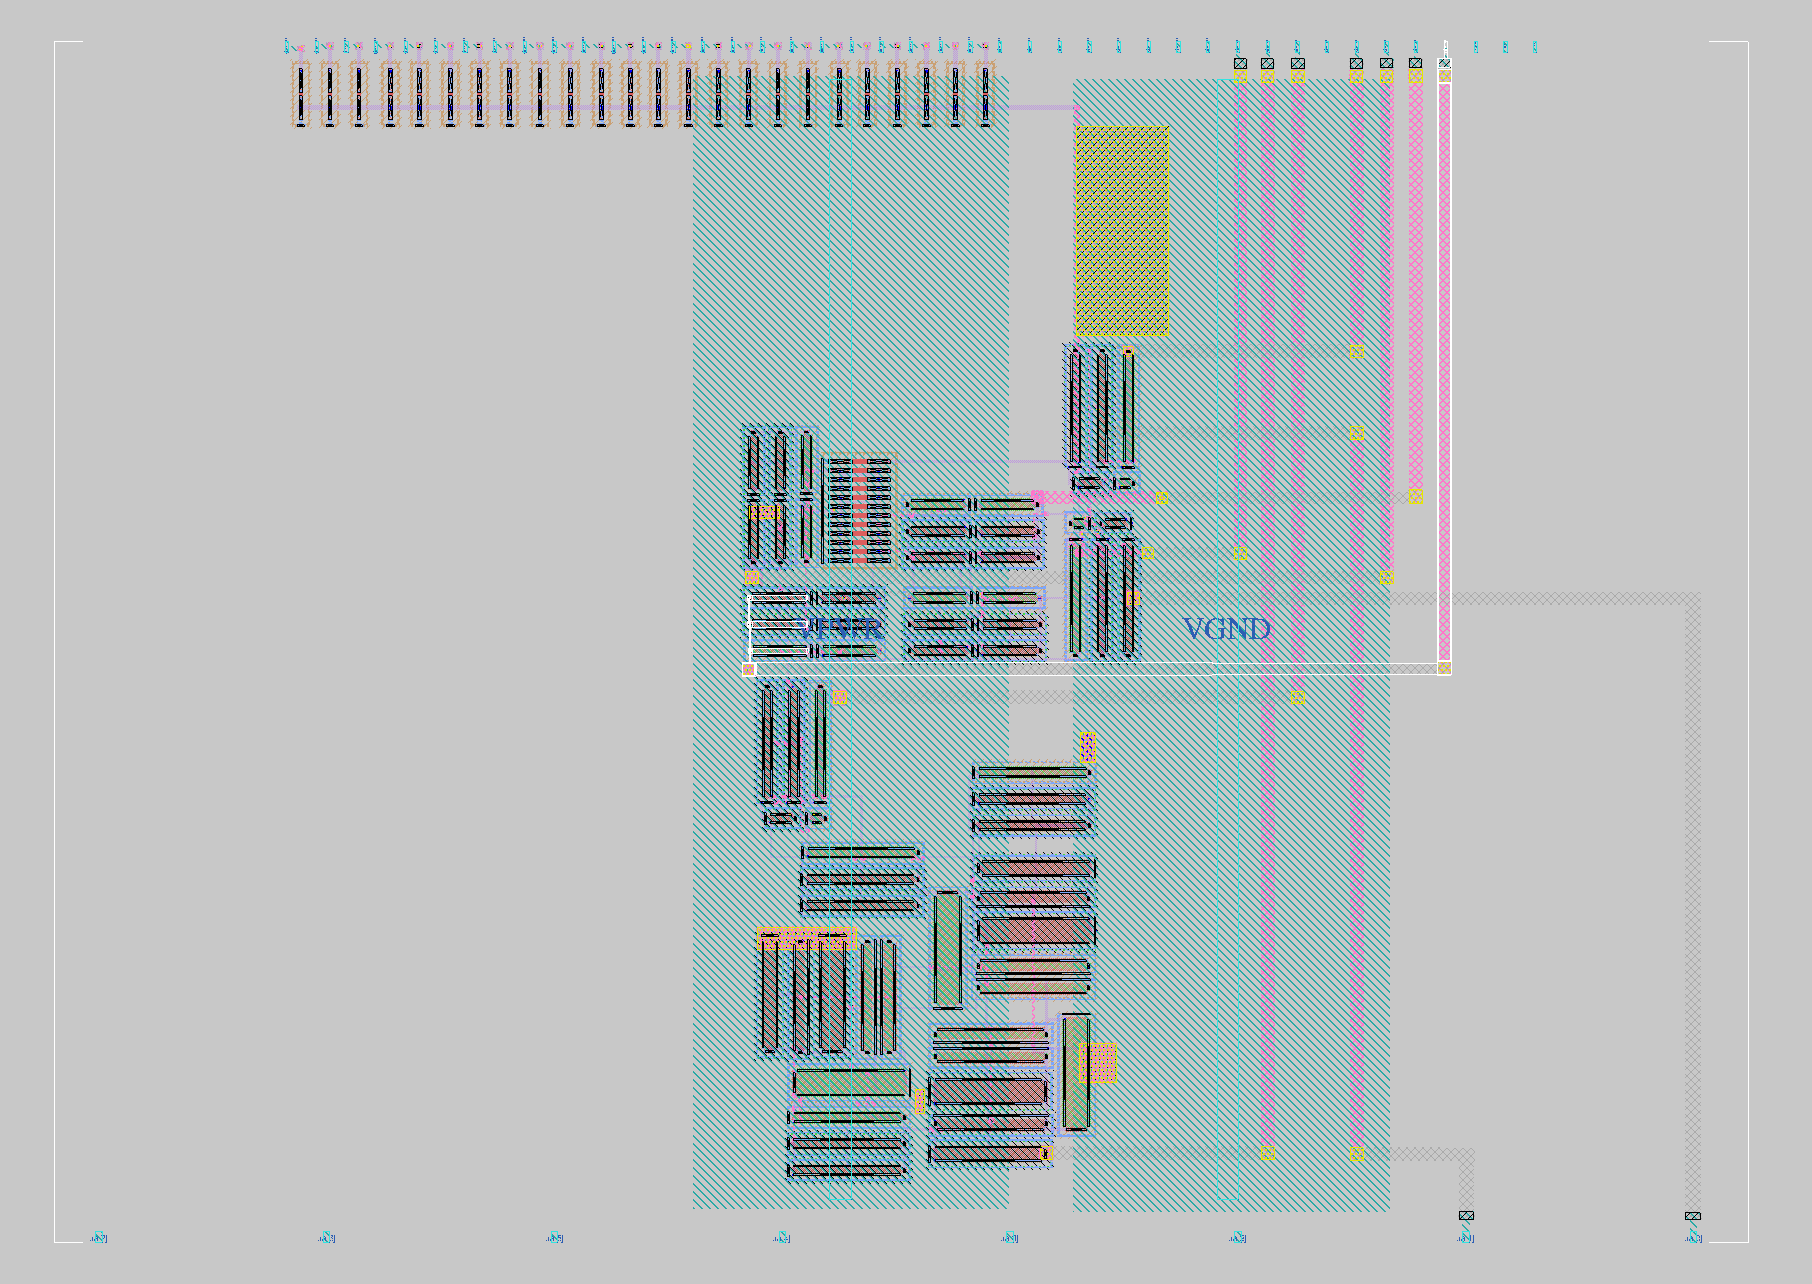
\includegraphics[width=\columnwidth]{./Figs/tt05_transmission_gate.png}
\caption{A ring oscillator and digital to analog converter (DAC) design submitted to Tiny Tapeout 5, with a transmission gate highlighted. This design was automatically placed and routed using an experimental analog place and route (P\&R) tool).}
\label{fig:transmission_gate_TT05}
\end{figure}

\section{Tiny Tapeout 6}
\label{sec:tinytapeout6}

For Tiny Tapeout 6 the Caravel harness will be replaced by OpenFrame~\cite{openframe}, an alternative harness provided by Efabless that uses the same padring but removes the RISC-V coprocessor.
This results in an additional \qty{5}{\mm\squared} of space for user designs, and 12 more IO pins which will be used for analog signals.

For increased safety, all designs will be power-gated. This allows designers to take more risks in their submissions, or to use custom flows not previously used in Tiny Tapeout.

Analog and mixed signal designs will be enabled by adding an analog multiplexer based on transmission gates~\cite{transmissiongates}. 
This allows up to 192 designs to share the analog pins between them.

Noise coupling between analog and digital power domains is a known concern. However, due to other limitations of our current setup including its limited number of low bandwidth analog interfaces, we target educational low to medium performance analog and mixed signal designs where noise coupling is a lesser concern.

Tiny Tapeout 6 opened for submissions in January 2024 and closes in April 2024. The final design will be submitted to Efabless chipIgnite 2404. Silicon is expected by October 2024.

\section{Circuit Boards}
\label{sec:circuit_board}
After manufacture Tiny Tapeout chips are mounted onto small carrier boards with 0.1~inch pin headers. These carriers allow people with limited surface mount technology (SMT) assembly experience to build their own demonstration boards around the chips.

The carrier fits onto the demonstration board shown in Fig.~\ref{fig:demonstration_board}. The demonstration board is designed primarily for ease of use by beginners, though offers enough flexibility for power users. As all signals are below \qty{50}{\MHz}, no special layout was needed in the design of the demonstration board.

The demonstration board provides:
\begin{itemize}
\item USB Type-C as a power connection,
\item \qty{1.8}{\V} and \qty{3.3}{\V} power supplies for core and IO,
\item \qty{20}{\MHz} oscillator,
\item Buttons for reset and single step clock,
\item An eight way DIP switch for inputs,
\item A nine way DIP switch for design selection,
\item A seven segment LED display for the outputs,
\item Headers for all IO, including two standard Digilent ports (PMOD),
\item A header to select the internal clock or to provide one externally,
\item A header to select an internal or external scan chain driver,
\item A header to engage an automatic clock divider in input pin zero.
\end{itemize}

\begin{figure}[!t]
\centering
\includegraphics[width=0.5\textwidth]{./Figs/tt02 pcb assembled.JPG}
\caption{The demonstration board, which has been recorded as Certified Open Source Hardware ES000040~\cite{oshwacertification}.}
\label{fig:demonstration_board}
\end{figure}

The move away from the scan chain architecture in Tiny Tapeout 3.5 and Tiny Tapeout 4 necessitated the design of a new demonstration board (Fig.~\ref{fig:TT04plus_demo_board}), which had to include an easy way to select a chosen design.
The Raspberry Pi RP2040 microcontroller was chosen as a coprocessor on the revised demonstration board, as it offers:

\begin{itemize}
\item Drag and drop firmware updates on any operating system,
\item MicroPython\cite{micropython} support, an ideal language and programming environment through which beginners can enable and test their designs (Fig.~\ref{fig:micropython_program}),
\item External memory emulation via programmable input output (PIO) and direct memory access (DMA) support.
\end{itemize}

\begin{figure}[!t]
\centering
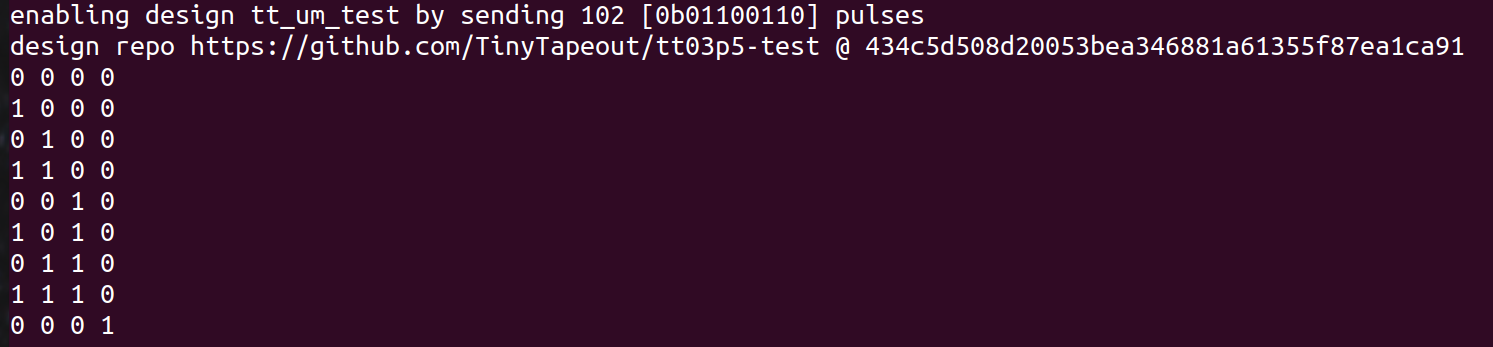
\includegraphics[width=\columnwidth]{./Figs/tt3p5 enable design.png}
\caption{A MicroPython program\cite{demofirmwaretest} enabling a chosen design, clocking it, and printing the results.}
\label{fig:micropython_program}
\end{figure}

\begin{figure}[!t]
\centering
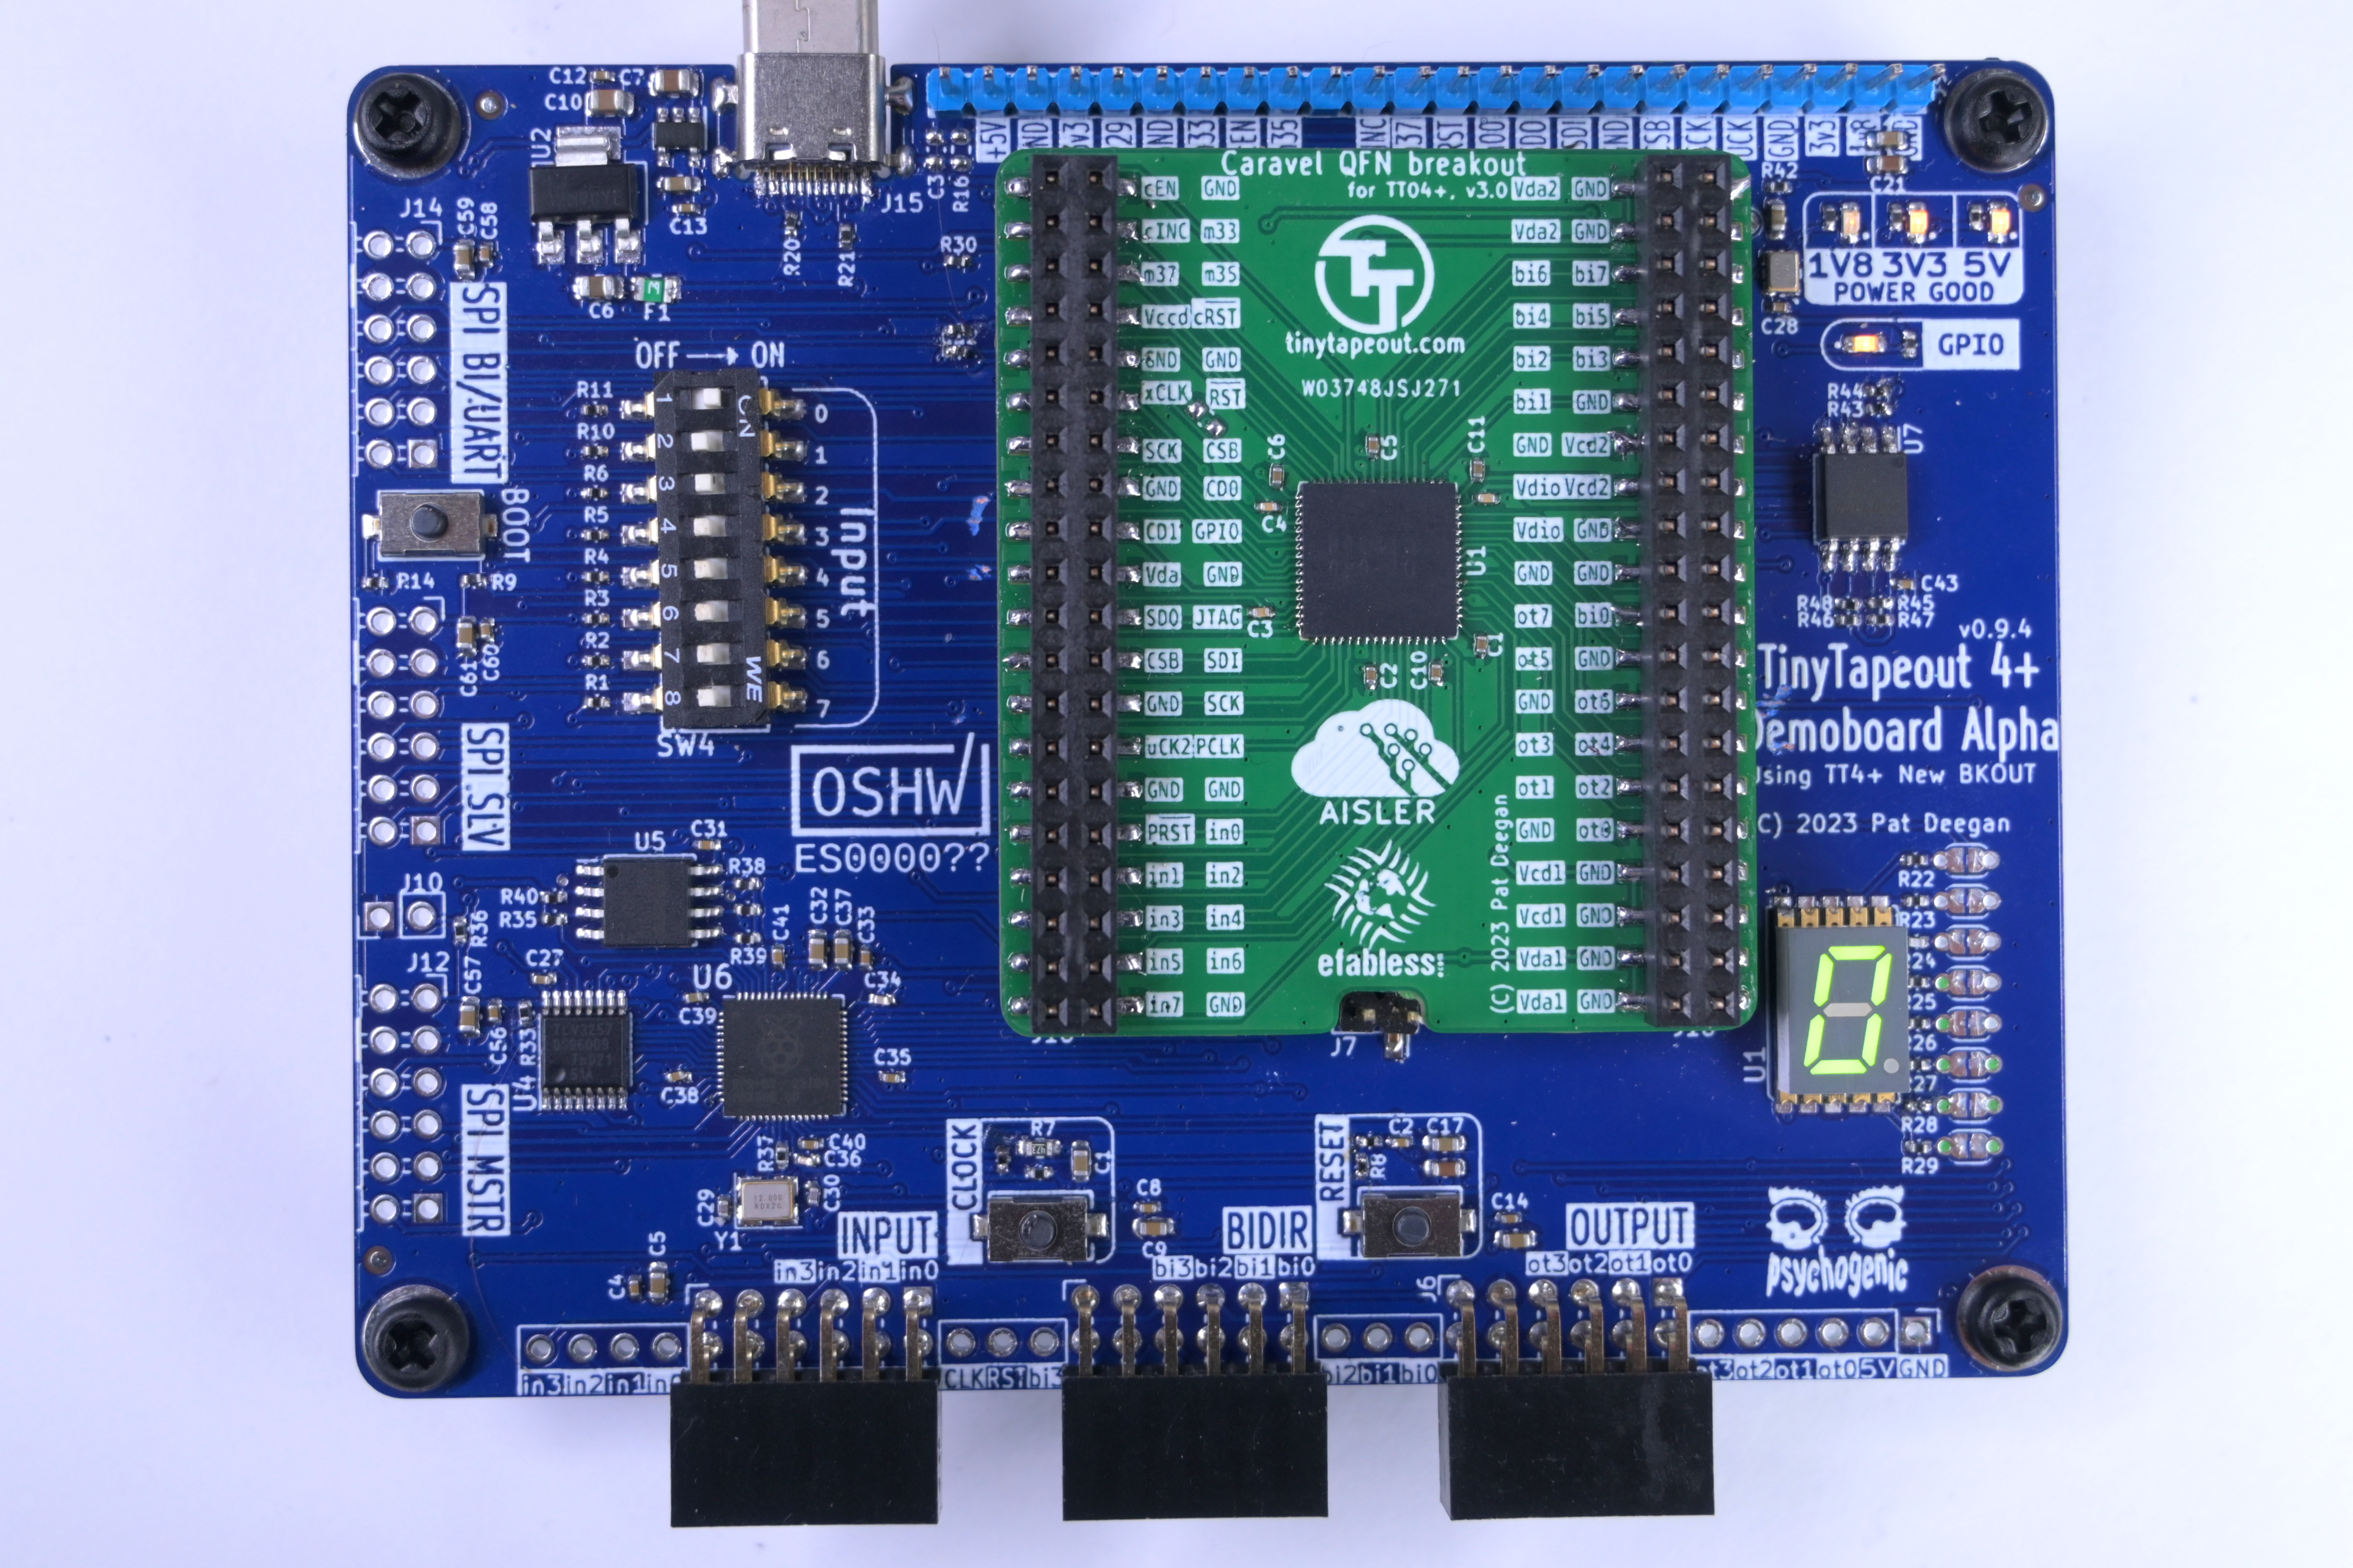
\includegraphics[width=\columnwidth]{./Figs/tt04-demoboard-top.jpg}
\caption{The Tiny Tapeout 4+ demonstration board\cite{tt04demoboard}.}
\label{fig:TT04plus_demo_board}
\end{figure}

An additional PMOD expansion port was added to the demonstration board for the bidirectional pins. The Tiny Tapeout community has begun to standardize on pinouts~\cite{pinouts}, making it easier to test each design.
A new repository was created to house user-contributed PMOD~\cite{awesomepmods} accessories, for example the VGA PMOD shown in Fig.~\ref{fig:user_contributed_VGA_PMOD}.

A further set of three PMOD expansion ports were added, mixing input and outputs, which allows the most common standard PMODs to be used with the demonstration board. For more information about the circuit board, pinout, and PMOD support see the repository~\cite{tt04demoboard}.

\begin{figure}[!t]
\centering
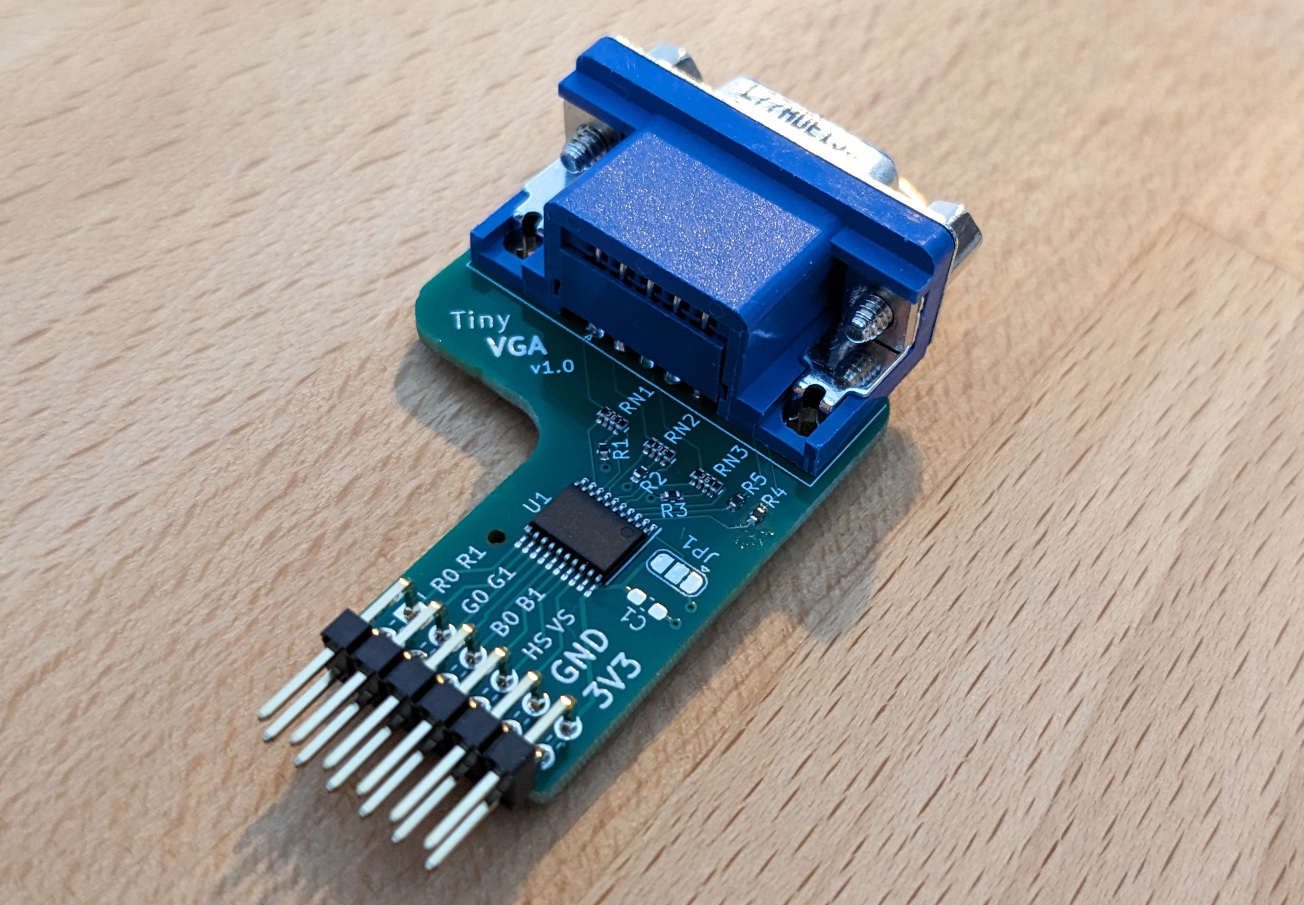
\includegraphics[width=\columnwidth]{./Figs/tiny_vga_pmod.jpg}
\caption{A user-contributed VGA output PMOD accessory for the demonstration board.}
\label{fig:user_contributed_VGA_PMOD}
\end{figure}

\section{Results and Measurements}
\label{sec:results}

Tiny Tapeout 2 chips were received in October 2023, 11 months after the chips were submitted for manufacture on the Efabless chipIgnite 2211Q shuttle.
The chips were tested for the first time on a public livestream~\cite{siliconalive}.
During this testing the chain was validated and a small number of the designs were demonstrated to be working.
In further testing following the livestream another 30 designs were tested and shown to be working.

\begin{figure}[!t]
\centering
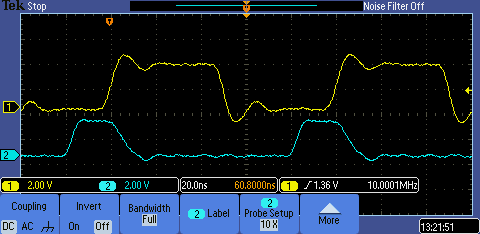
\includegraphics[width=\columnwidth]{./Figs/tt02_clock_out.png}
\caption{Measurement from Tiny Tapeout 2 silicon, with input clock in yellow and the distorted output clock in blue.}
\label{fig:TT02_clock_out}
\end{figure}

After measuring the clock asymmetry (Fig.~\ref{fig:TT02_clock_out}) and maximum frequency it was decided to run the production boards with a \qty{20}{\MHz} oscillator, resulting in a \qty{10}{\MHz} scan chain clock and a \qty{5}{\kHz} IO update rate in order to maximize stability.

Some Tiny Tapeout 2 designs did not function as expected; in most cases this was determined to be due to faults in the submitted design.

Of the designs submitted 82 used the Verilog HDL, 64 were created using the Wokwi graphical editor, and six used alternative HDLs including VHDL, Amaranth~\cite{amaranth}, and Chisel~\cite{chisel}.

Some of the designs created using Wokwi using combinational logic in clock paths (Fig.~\ref{fig:failed_design_comb_logic}) worked in simulation but failed in hardware.
This was determinted to be due to the lack of timing data in the simulation, and was not detected by STA because the clock paths were not known. A detailed analysis on these failures has yet to be carried out.

\begin{figure}[!t]
\centering
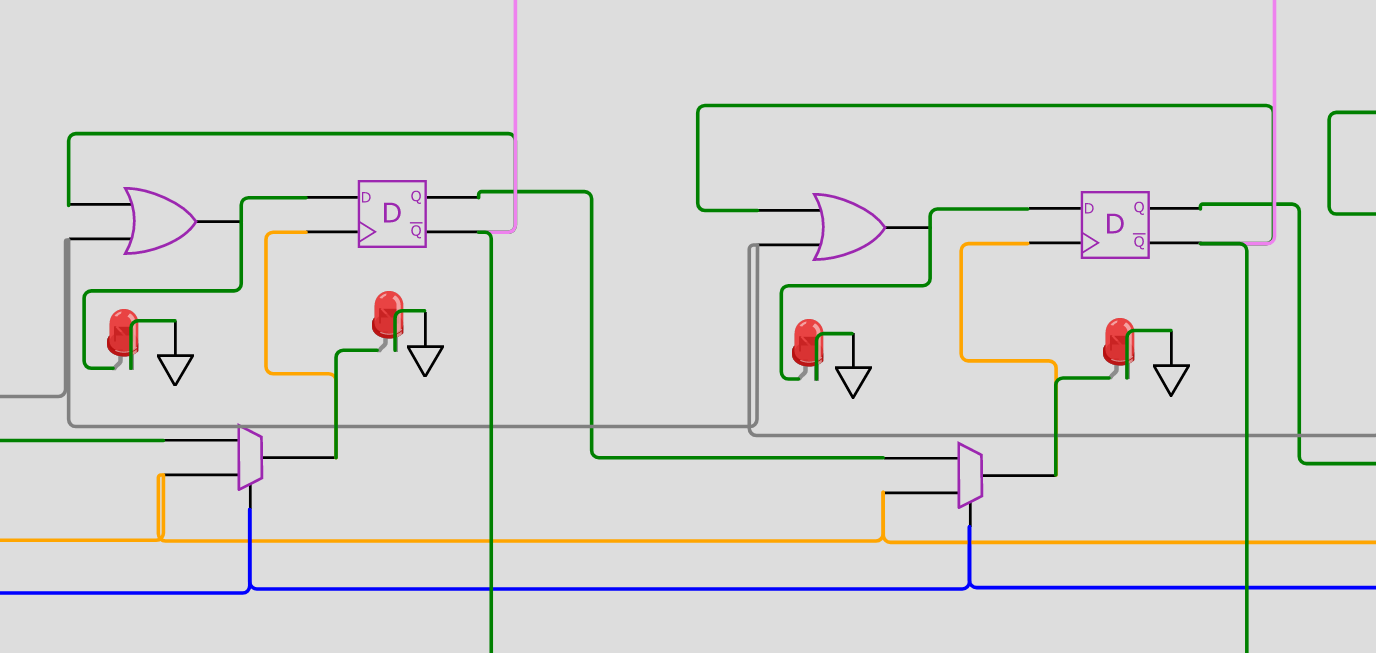
\includegraphics[width=\columnwidth]{./Figs/wokwi mux clock logic.png}
\caption{Combinational logic in the clock path of one of the failed designs.}
\label{fig:failed_design_comb_logic}
\end{figure}

PCBs were assembled and shipped to customers in January 2024. Around 50 designs have been tested and shown to be working.

Silicon from Tiny Tapeout 3 production was received in January 2024. The updated scan chain design shows a more symmetric output clock at the end of the chain (Fig.~\ref{fig:TT03_silicon_measurement}). The improved clock symmetry will allow for the use of a faster scan chain clock, resulting in a faster update frequency.

\begin{figure}[!t]
\centering
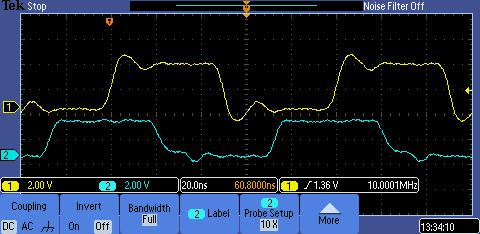
\includegraphics[width=\columnwidth]{./Figs/tt03_clock_out.png}
\caption{Measurement from Tiny Tapeout 3 silicon.}
\label{fig:TT03_silicon_measurement}
\end{figure}

Some Tiny Tapeout 3.5 designs have already been validated, including a VGA clock project (Fig.~\ref{fig:VGA_clock_design_TT03_5_silicon}) which takes advantage of the new higher speed IO.

The overhead of multiplexing multiple tiles makes power consumption of the infrastructure only a minor concern at this point. No direct comparison of the power consumption impact of the multiplexer over the previous scan chain architecture is available at the time of writing. The motivation of the multiplexer approach, however, was to substantially increase the bandwidth of the IOs.

After Tiny Tapeout 3.5 silicon was received and tested, the worst round trip latency was measured to be \qty{20}{\ns} as shown in Fig~\ref{fig:round_trip_latency_rising_edge} and \ref{fig:round_trip_latency_falling_edge}.

\begin{figure}[!t]
\centering
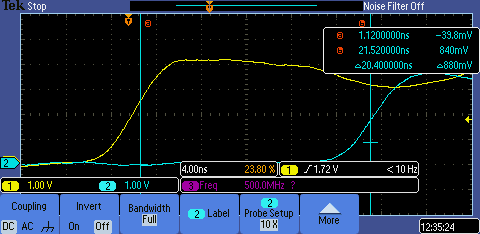
\includegraphics[width=\columnwidth]{./Figs/tt3p5 rising latency.PNG}
\caption{The Tiny Tapeout 3.5 round trip latency on a rising edge, measured at about \qty{20}{\ns}.}
\label{fig:round_trip_latency_rising_edge}
\end{figure}

\begin{figure}[!t]
\centering
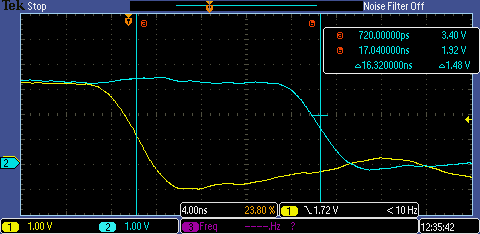
\includegraphics[width=\columnwidth]{./Figs/tt3p5 falling latency.PNG}
\caption{The Tiny Tapeout 3.5 round trip latency on a falling edge, measured at about \qty{16}{\ns}.}
\label{fig:round_trip_latency_falling_edge}
\end{figure}

\begin{figure}[!t]
\centering
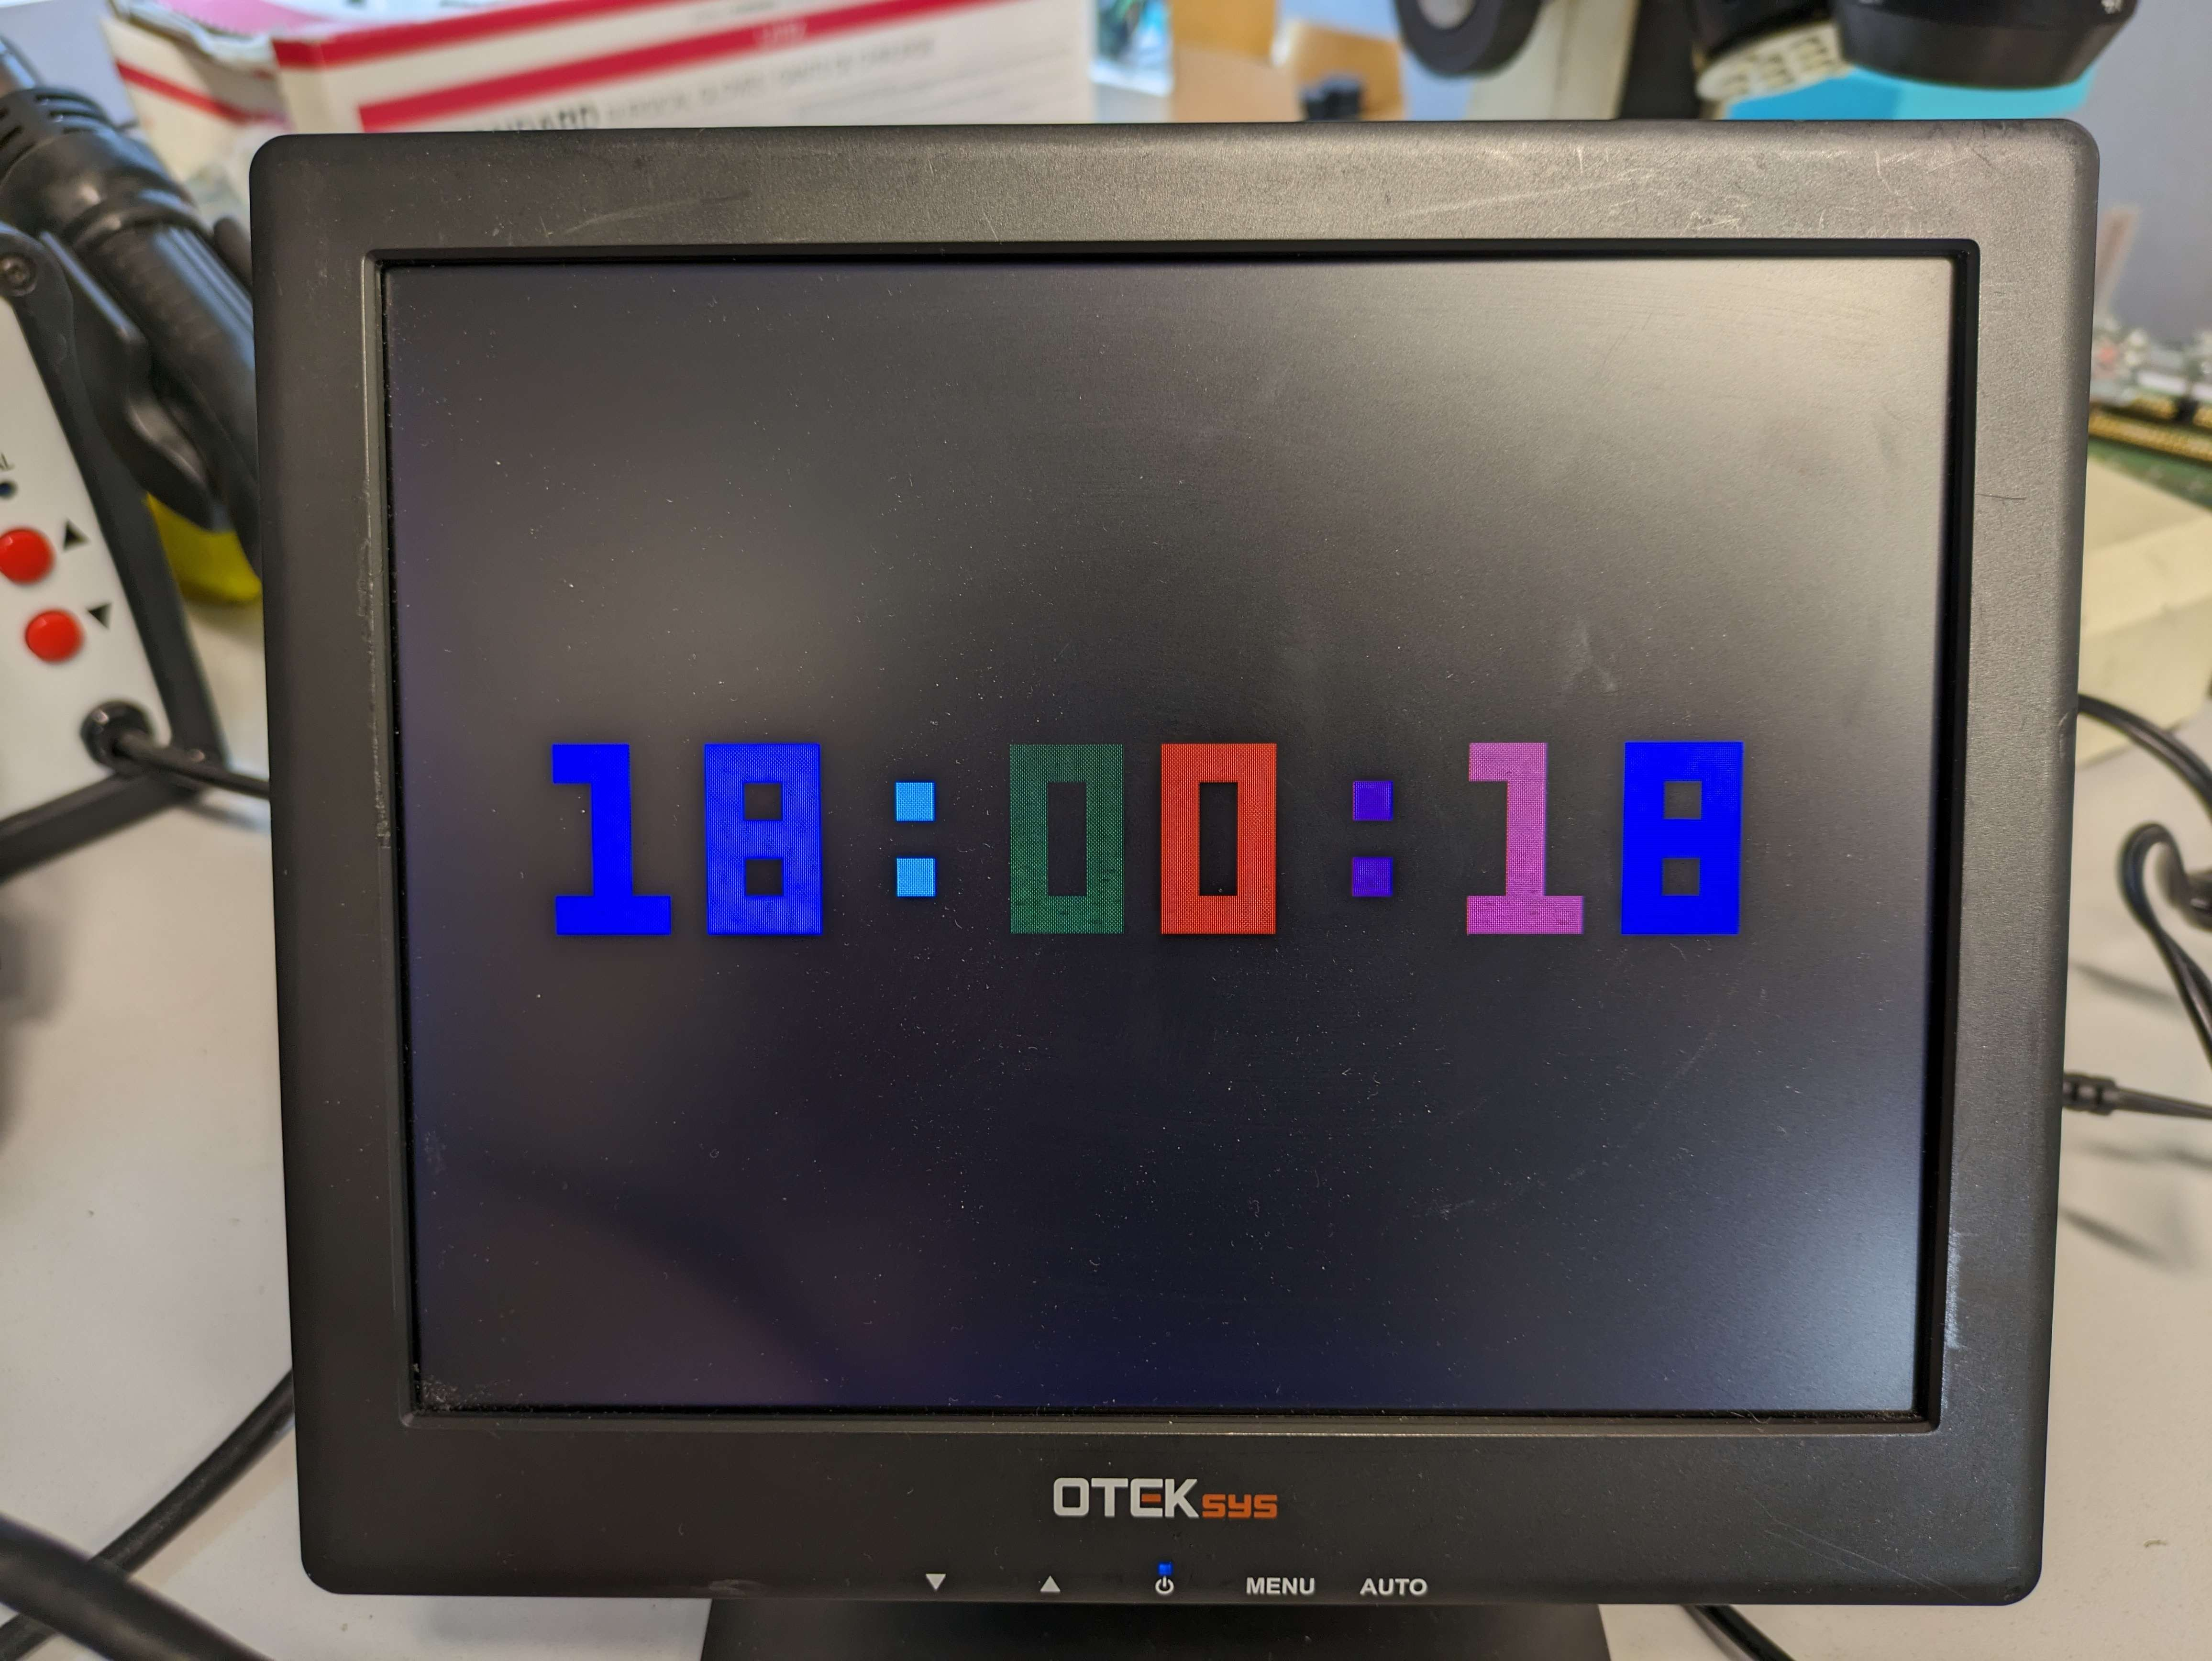
\includegraphics[width=\columnwidth]{./Figs/tt3p5 vga clock.jpg}
\caption{A VGA clock design running on Tiny Tapeout 3.5 silicon.}
\label{fig:VGA_clock_design_TT03_5_silicon}
\end{figure}

\section{Silicon Showcase}
\label{sec:silicon_showcase}

A curated list showcasing the types of designs possible through Tiny Tapeout is provided below:

\begin{itemize}
    \item Serial FPGA~\cite{showcaseserialfpga}, a one fracturable 5-LUT that receives FPGA LUT configuration frames, serially evaluates LUT inputs and LUT outputs.
    \item Synthesizable digital temperature sensor~\cite{showcasetempsense}. By creatively twisting the use of a tristate-inverter (EINVP) a voltage DAC is built. This voltage-mode DAC is used to bias an NMOS into subthreshold operation to discharge the input capacitor of an inverter. Since the subthreshold current of a MOSFET is a strong function of temperature, the resulting delay time is also a strong function of temperature, thus a digital temperature sensor is built.
    \item 395 standard cells with multiplexer~\cite{showcasemicrotapeout}, this design contains a copy of most standard cells in the sky130_fd_sc_hd library along with a multiplexing mechanism that allows exposing any of them to the input/output pins.
    \item FM transmitter with I2S input~\cite{showcasefmtx}. This design takes an audio signal and modulates it to a higher carrier frequency, using FM modulation. The modulator in this design is based on a numerically controlled oscillator (NCO) with several modifications.
    \item USB Full Speed device~\cite{showcaseusb}. This is a hardware implementation of a USB device end hardware interface, should be compliant with USB1.1 FS/LS (not HS).
    \item A Linux capable RISC-V CPU~\cite{showcasekianv}. This design is an RV32IMA RISC-V processor that aims to boot and run uLinux.
\end{itemize}

An index of all designs submitted to Tiny Tapeout can be found at \url{TinyTapeout.com/runs/}~\cite{tinytapeoutruns}.

%\section{Conclusion}
\label{sec:conclusion}

Tiny Tapeout runs 1 through 6 inclusive have demonstrated demand for more accessible entry points into chip design and fabrication. By lowering both the technical and financial barriers to entry, Tiny Tapeout is enabling hobbyists, educators, and others traditionally excluded to design and produce their own ASICs and to receive physical hardware in return.

Key to the success of the project is the inclusion of all projects from a given run on a single chip, going a step beyond the multi project wafer approach common in the industry today. By fabricating every design from a given run on every chip produced the cost can be shared between all participants, while the educational benefits are increased by allowing participants to experiment with others' designs in addition to their own.

Results from Tiny Tapeout runs for which hardware is available have proven the concept, and issues highlighted in earlier runs have been addressed for subsequent runs. The addition of analog and mixed circuit capabilities in Tiny Tapeout 6, the latest run at the time of writing, opens a new front for experimentation and education.

Community engagement in Tiny Tapeout has been strong with \qty{756} designs submitted over the first five shuttles. An online chat server for participants has \qty{1200} members and there are \qty{2600} subscribers to the project's mailing list.

The number of participants identifying as hobbyists, students, and teachers shows a demand for accessible chip design and manufacturing capabilities from groups largely overlooked by traditional approaches. As refinement of the Tiny Tapeout documentation and tools continues we expect an increase in participants who are trying chip design for the first time.


% can remove
%\section{Conclusions}
\label{sec:conclusions}
The conclusion goes here.

\section{Acknowledgements}
\label{sec:acknowledgements}

\begin{enumerate}
    \item Uri Shaked for Wokwi development and lots more.
    \item Sylvain Munaut for help with scan chain improvements.
    \item Mike Thompson and Mitch Bailey for verification expertise.
    \item Jix for formal verification support.
    \item Proppy for help with GitHub actions.
    \item Maximo Balestrini for the amazing renders and the interactive GDS viewer.
    \item Harald Pretl for advice and analog support.
    \item The team at YosysHQ and all the other open source EDA tool makers.
    \item Efabless for running the shuttles and providing OpenLane and sponsorship.
    \item Tim Ansell and Google for supporting the open source silicon movement.
    \item Pat Deegan for PCB development.
    \item TinyTapeout community for all their contributions.
    \item Zero to ASIC course community for all your support.
\end{enumerate}




%%%%%%%%% -- BIB STYLE AND FILE -- %%%%%%%%
\bibliographystyle{IEEEtran}
\bibliography{IEEEabrv,references.bib}
%%%%%%%%%%%%%%%%%%%%%%%%%%%%%%%%%%%%

\end{document}
